% Hamad Medical Corporation
% Georges Younes

\section{System Integration and Demonstration Prototype}
\label{sec:system_integration}

\subsection{Console Setup}
\label{ssec:console_setup}
We developed software with the following features:
\begin{enumerate}
  \item Able to load and render \acr{dicom} images, organ models (derived from \acr{mri} images), and \acr{cad} models of surgical robotic instruments (which include stereoscopic camera, EndoWrist instruments, and trocars),
  \item The user can select and manipulate the positions of the trocars with Fulcrum effect simulated at the incision point (\autoref{fig:simulation_setup}), and
  \item Using the software, one can define the starting scenario for patient-specific simulation of a surgical procedure (\autoref{fig:stereoscopic_console}).
\end{enumerate}

\begin{figure}
  \centering%
  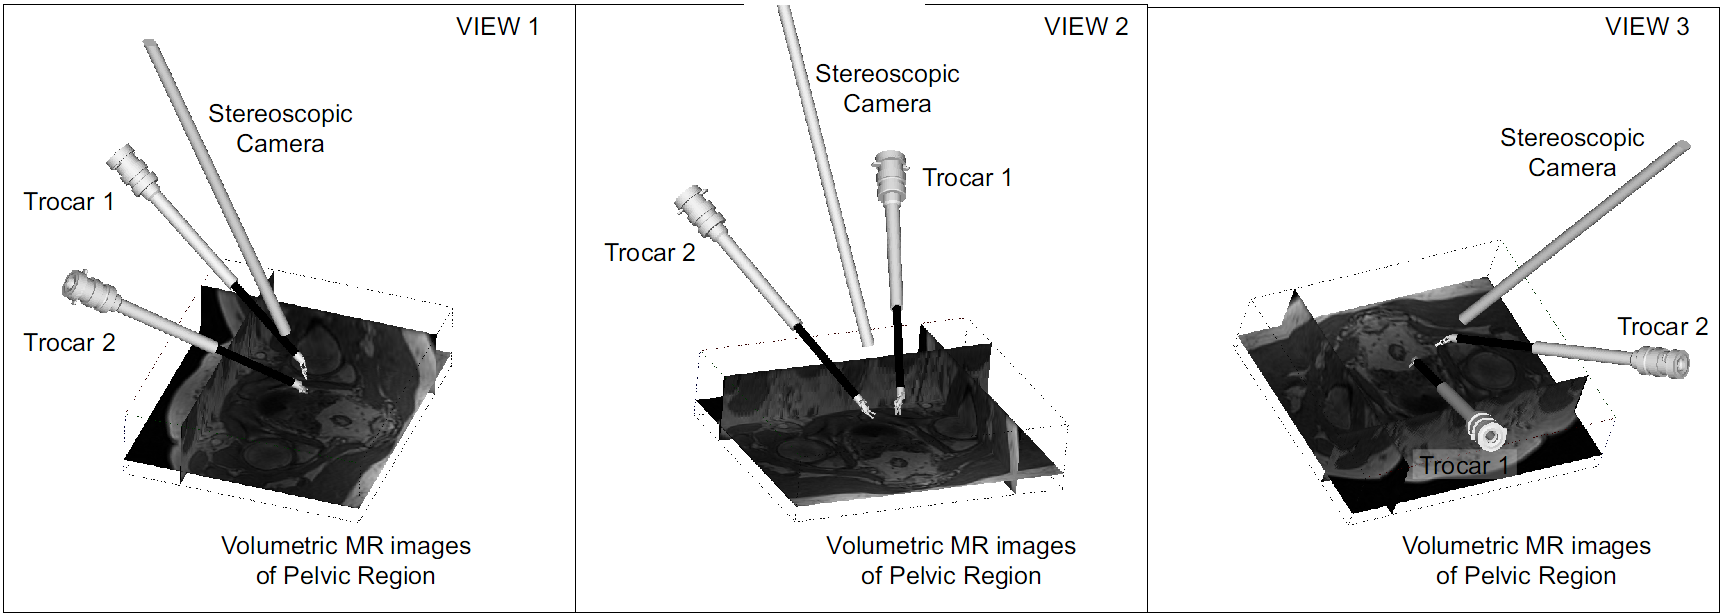
\includegraphics[width=1.0\linewidth]{integration/multiple_views_fusion}
  \caption{Simulation setup rendered by software from different viewpoints}
  \label{fig:simulation_setup}
\end{figure}

\begin{figure}
  \centering%
  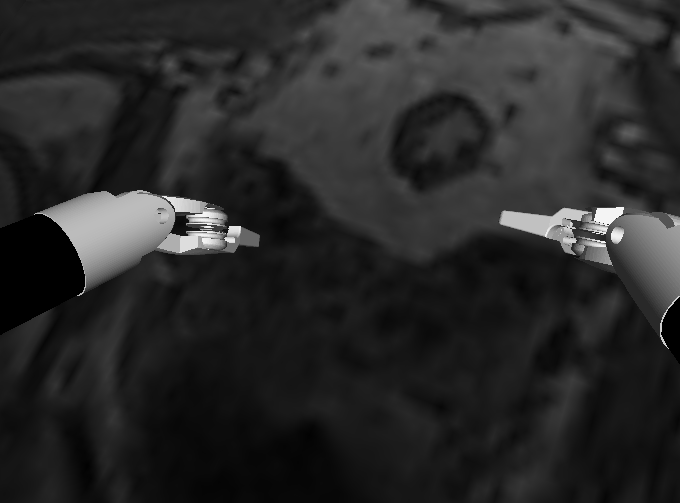
\includegraphics[width=0.6\linewidth]{integration/console_view}
  \caption{View from stereoscopic camera as seen from surgeon’s console}
  \label{fig:stereoscopic_console}
\end{figure}

\hrule%

\subsection{Stereoscopic Rendering}
\label{ssec:stereo_rendering}

We have implemented true off-axis stereoscopic rendering as shown below where a two tubes are rendered in Red-Cyan Anaglyph \acr{3d}.

\begin{figure}
  \centering%
	\frame{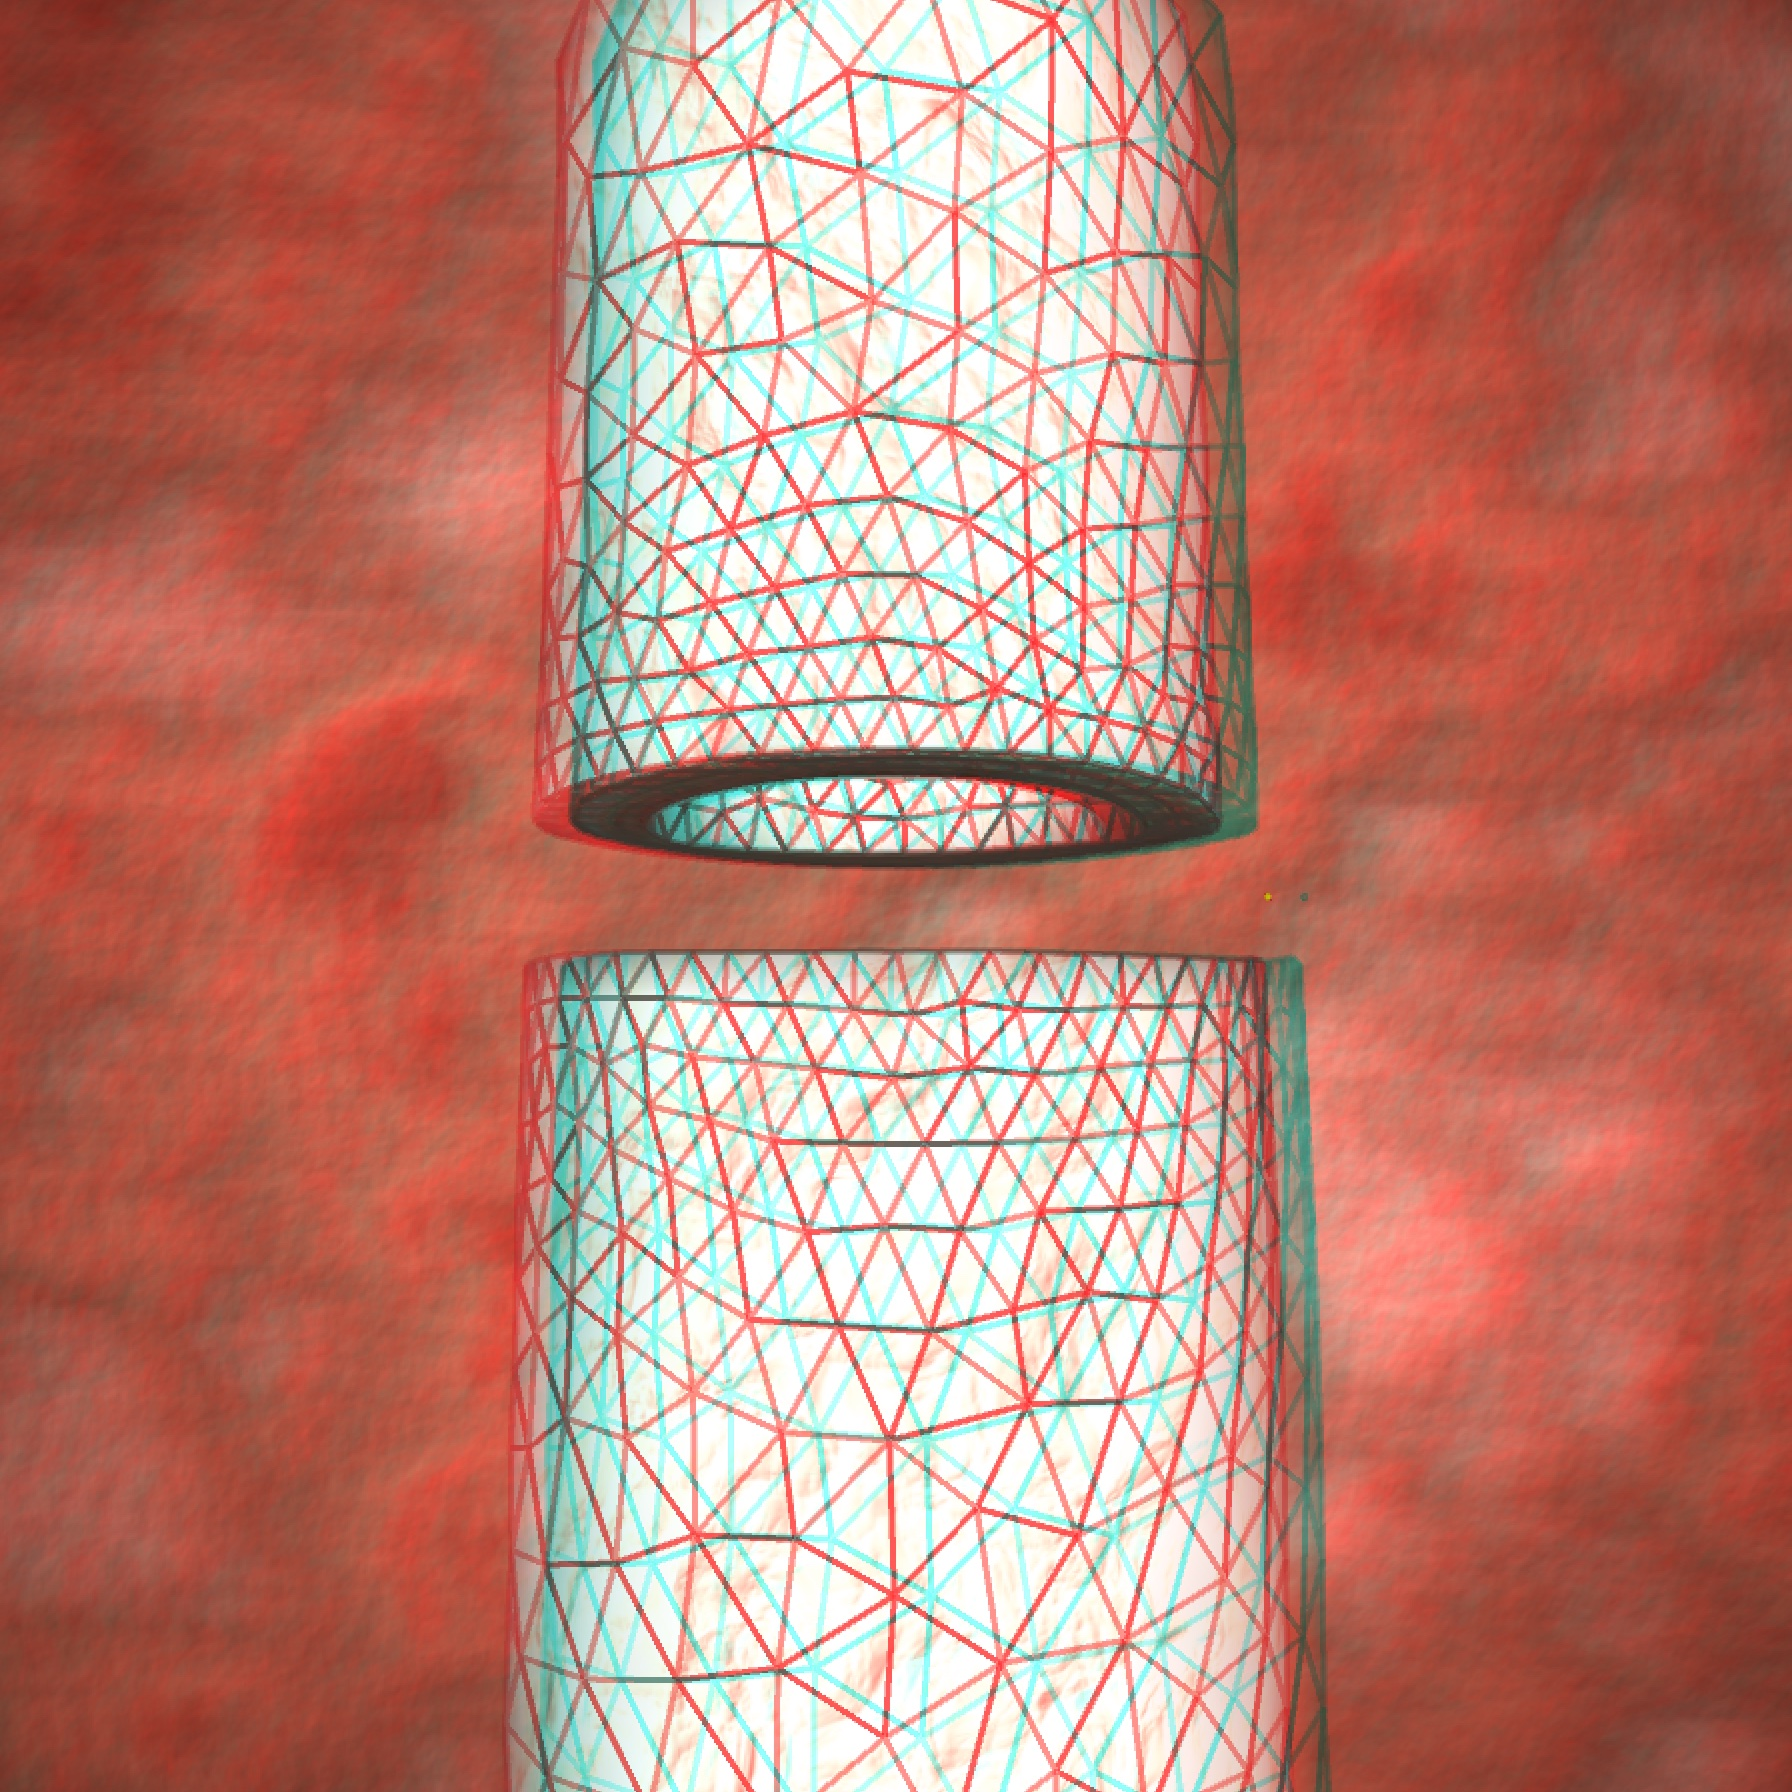
\includegraphics[width=0.5\linewidth]{integration/stereoscopic_anaglyph_red_cyan_rendering}}
	\caption{---}
	\label{fig:stereo}
\end{figure}

\hrule%

\subsection{Cross-Platform Integration}
\label{ssec:cross}
We have created a cross-platform pipeline for continuous integration between our different collaborating teams. Our prototype compiles (using CMake) and runs on all three major platforms: Windows (10 1909 Professional), macOS (Catalina), and GNU/Linux (Fedora 31 and Ubuntu 19.10). We're hosting our private source control repository with \href{https://gitlab.com}{GitLab} to streamline the code access and allow us to experiment with different branches, and are currently working on automating our builds if we were to have more collaborators on board or disseminate our product in the future.

\subsection{User Interface}
\label{ssec:console}
We're using robust C++11 libraries and frameworks such as GLFW, GLM, CGAL, Boost, and Eigen, and rendering using OpenGL's Core Profile. We've added support for a bimanual interface using a pair of 3Dconnexion Spaceballs, shown in \autoref{fig:spaceball}, and we're also collecting all the various metrics outlined in Aim 5. This will allow to replay the procedures as they happened too.

\begin{figure}
  \centering%
  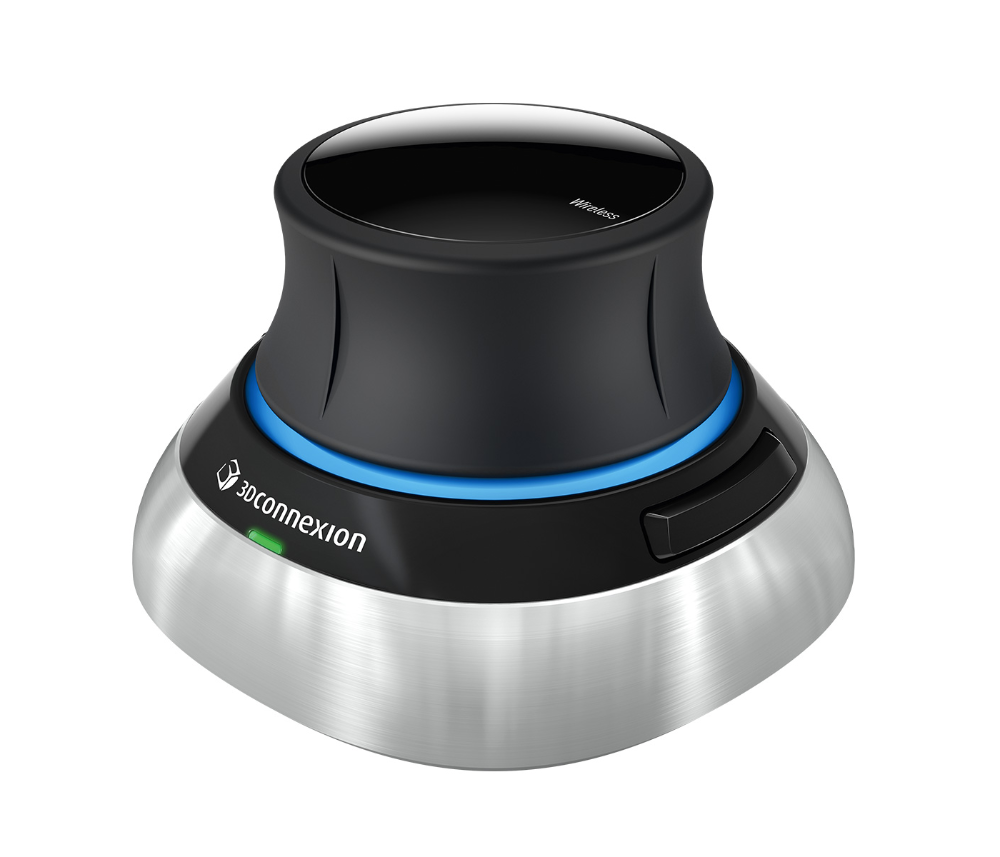
\includegraphics[width=0.32\linewidth]{integration/spaceball_iso_right}
  \hfill%
  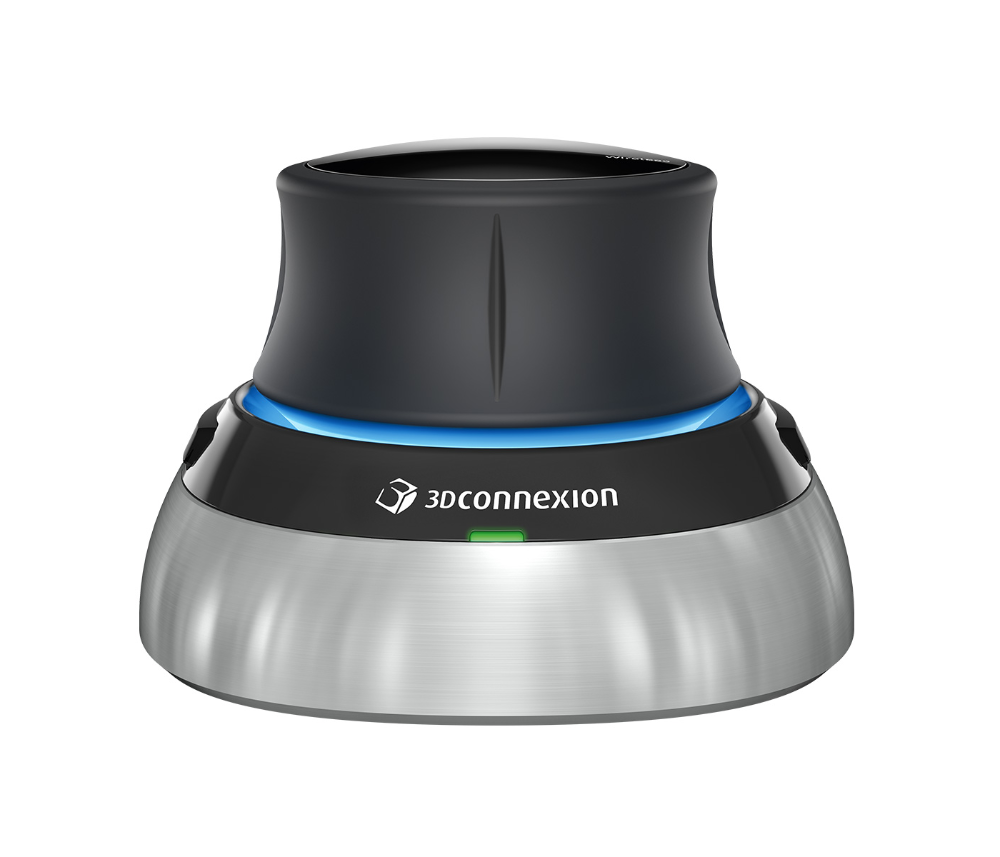
\includegraphics[width=0.32\linewidth]{integration/spaceball_front}
  \hfill%
  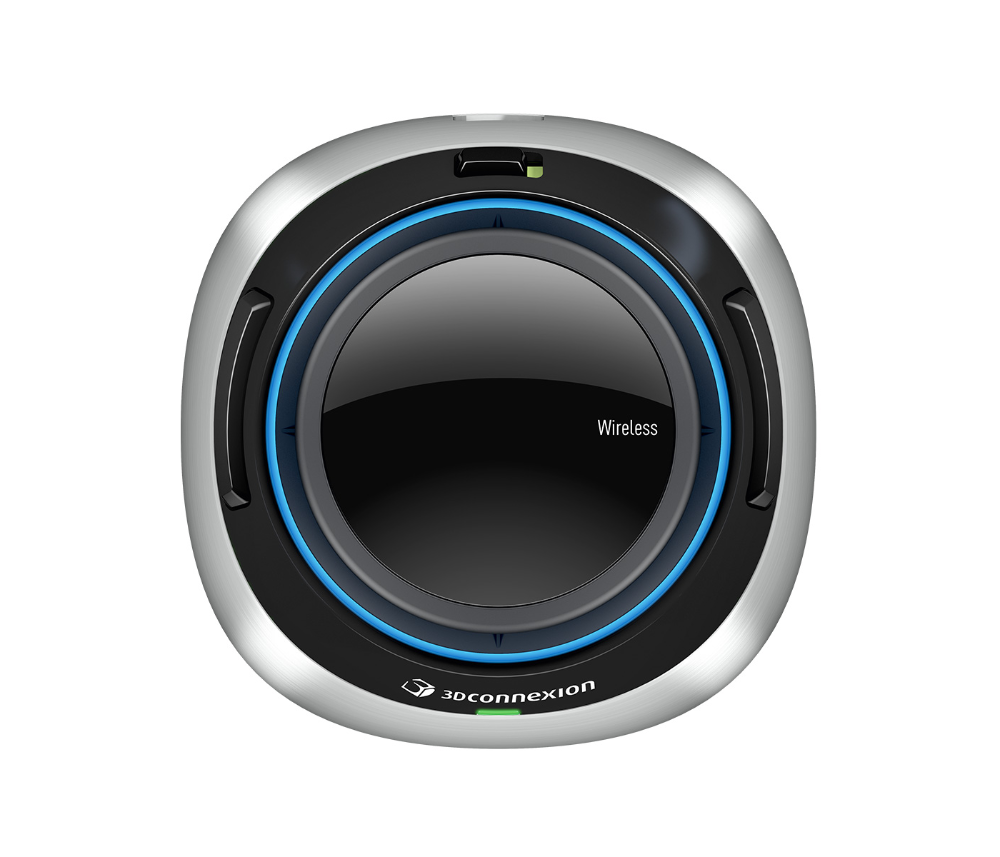
\includegraphics[width=0.32\linewidth]{integration/spaceball_top}
  \caption{Three views of the 3Dconnexion SpaceBall}
  \label{fig:spaceball}
\end{figure}

\begin{figure}
  \centering%
  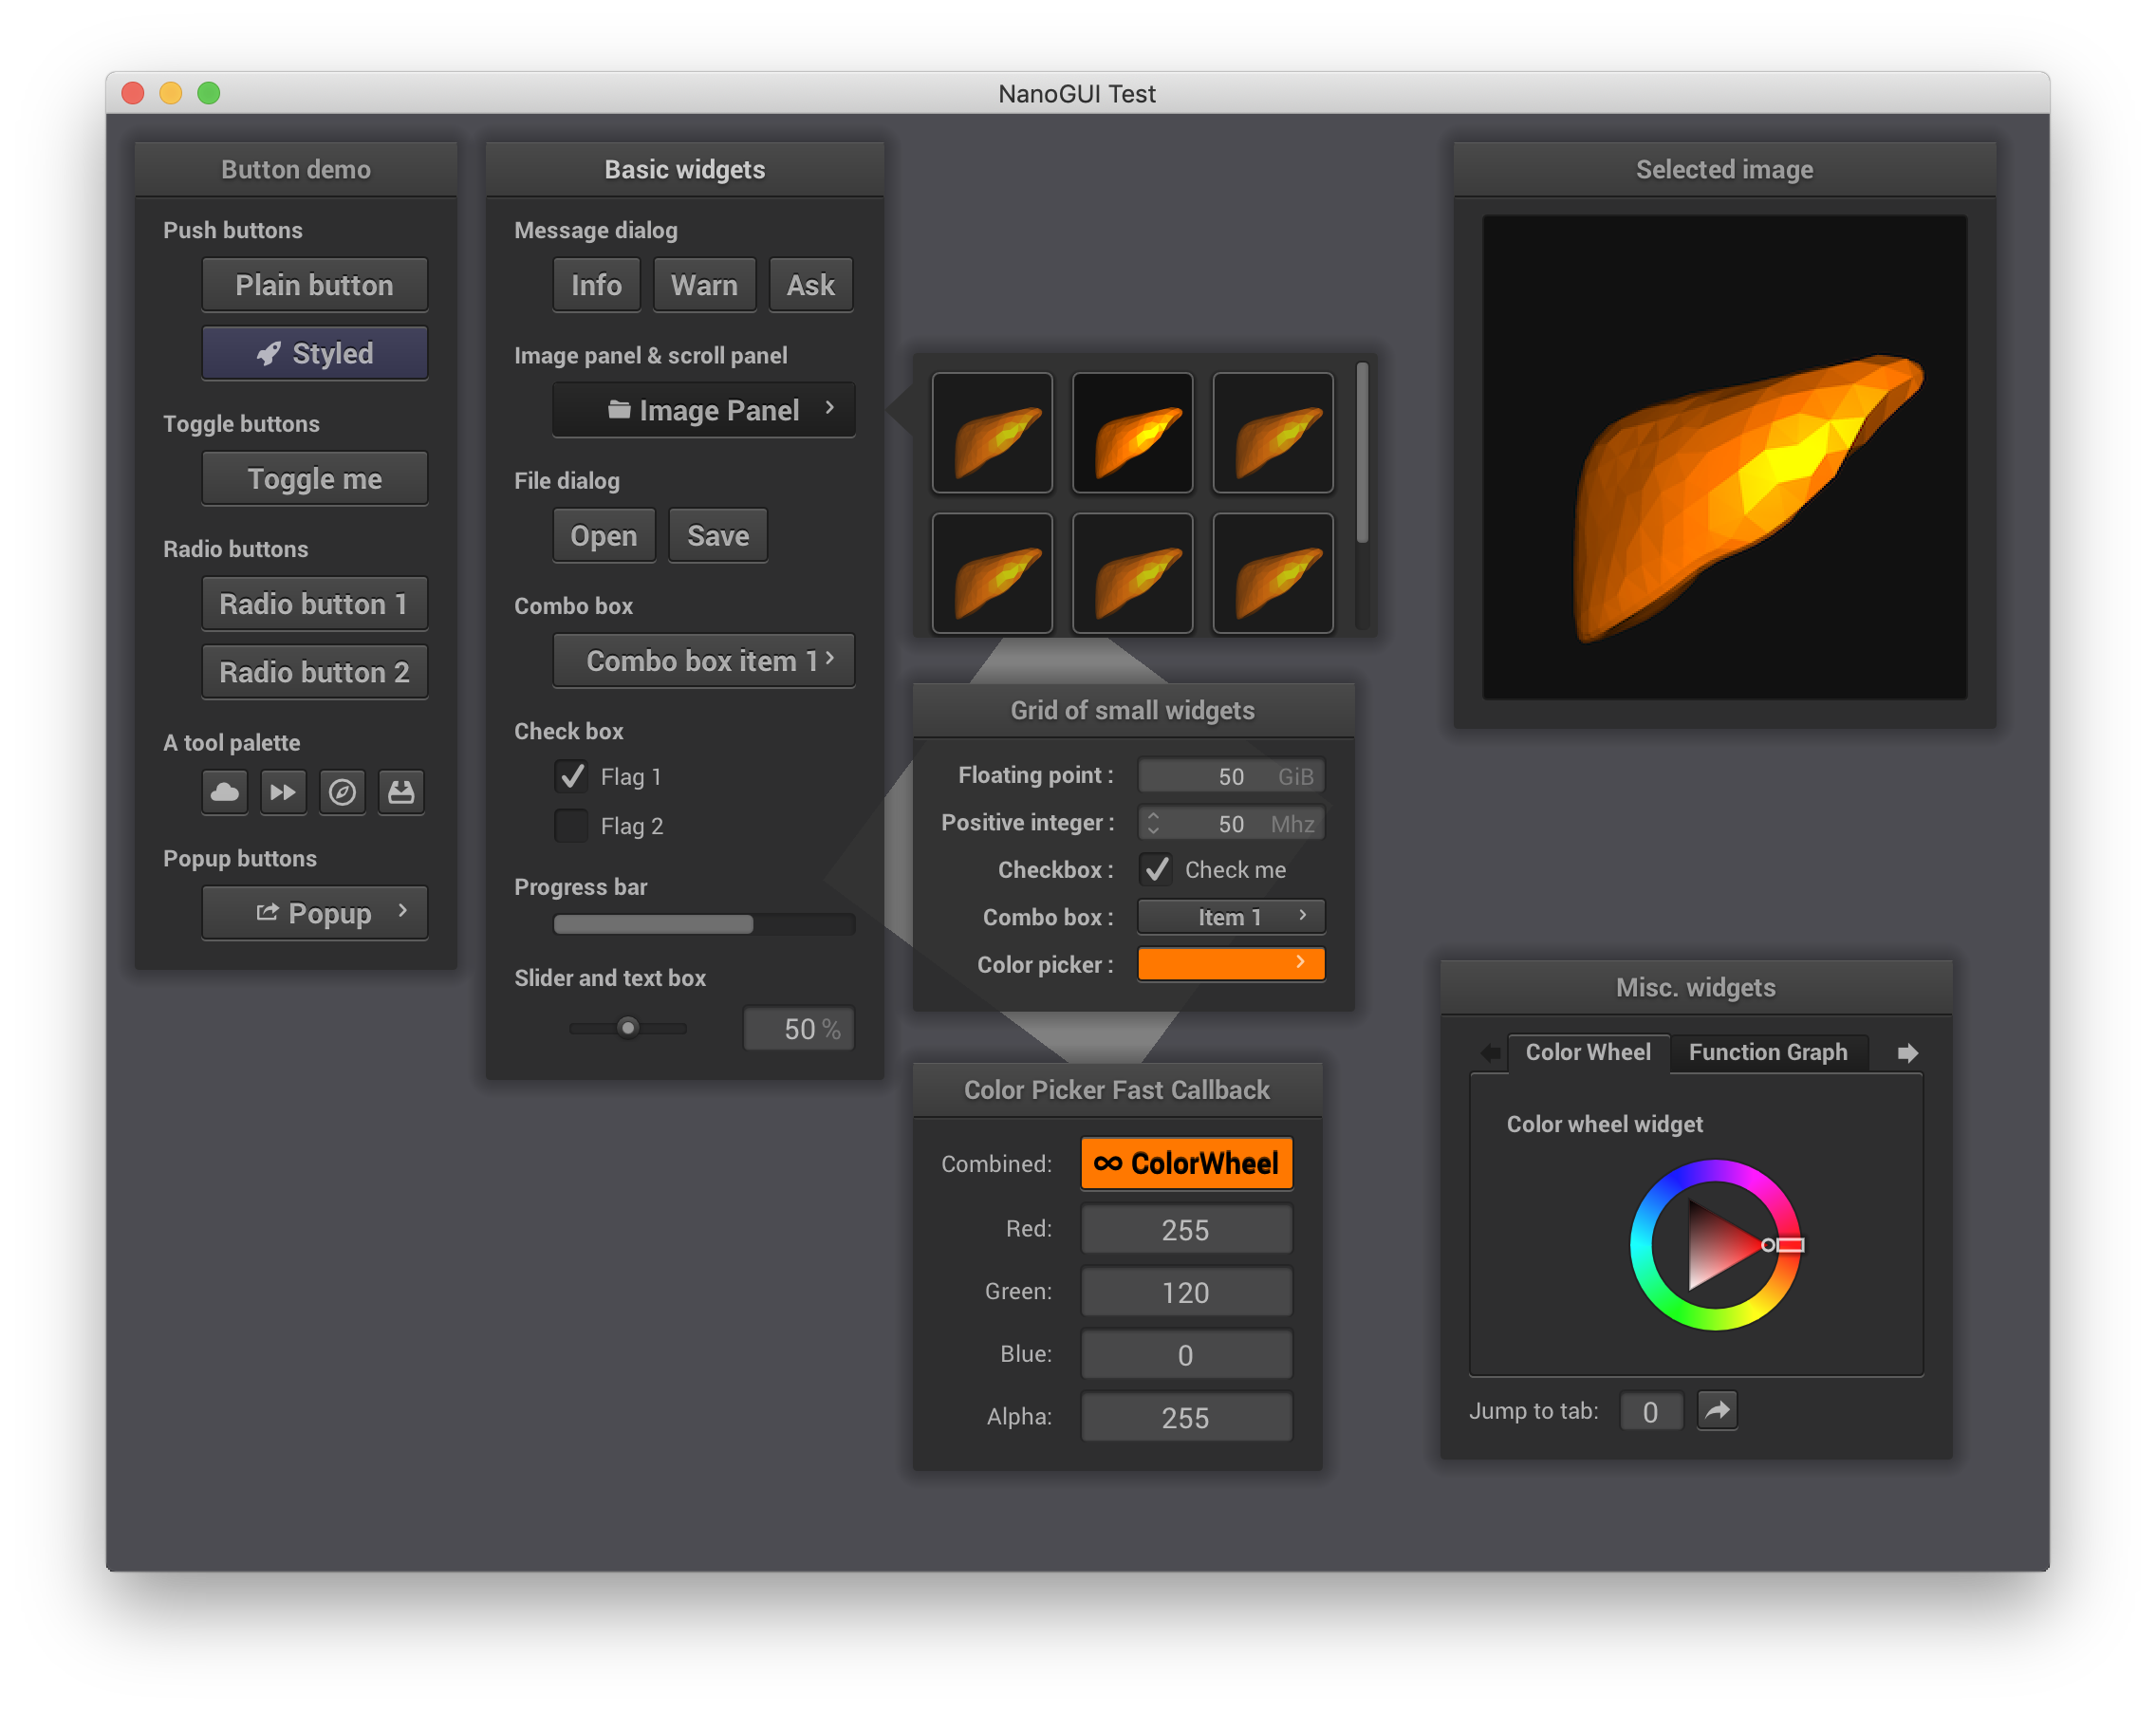
\includegraphics[width=\linewidth]{integration/nanogui_sample}
  \caption{NanoGUI widget library example}
  \label{fig:nanogui}
\end{figure}

We've added support for \acr{hud} using NanoGUI widgets. This'll allow us to display user-friendly notifications and queues, and implement the mockups designed in Aim 5. A sample of the what the library is capable of is shown in \autoref{fig:nanogui}.

An interactive animation from our system integrating the outcomes from the various aims is available at \url{https://www.dropbox.com/s/ax9kmdhaeq91puc/scind_gui.mp4}.

\subsection{Haptic Control}
\label{ssec:haptic}
We're using the OpenHaptics framework and the 3D Systems Touch, shown in \autoref{fig:touch}, to render the forces relayed from the finite element method kernel from Aim 2.

\begin{figure}
  \centering%
  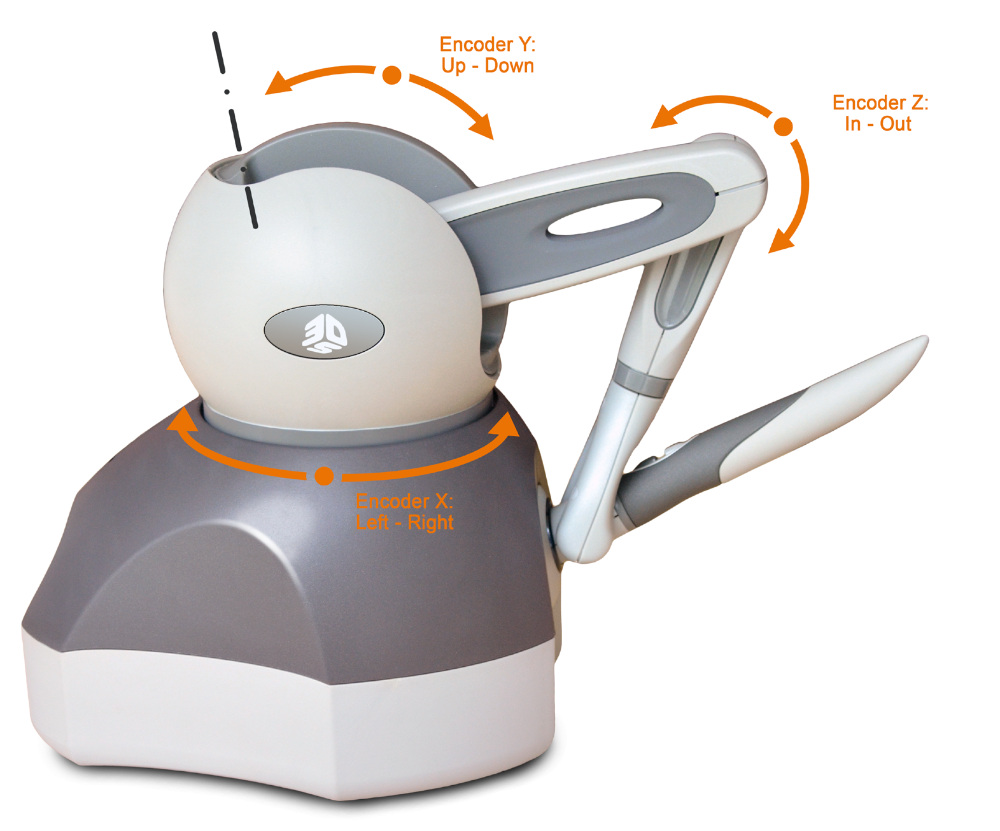
\includegraphics[width=0.48\linewidth]{integration/touch_hero_encoders}
  \hfill%
  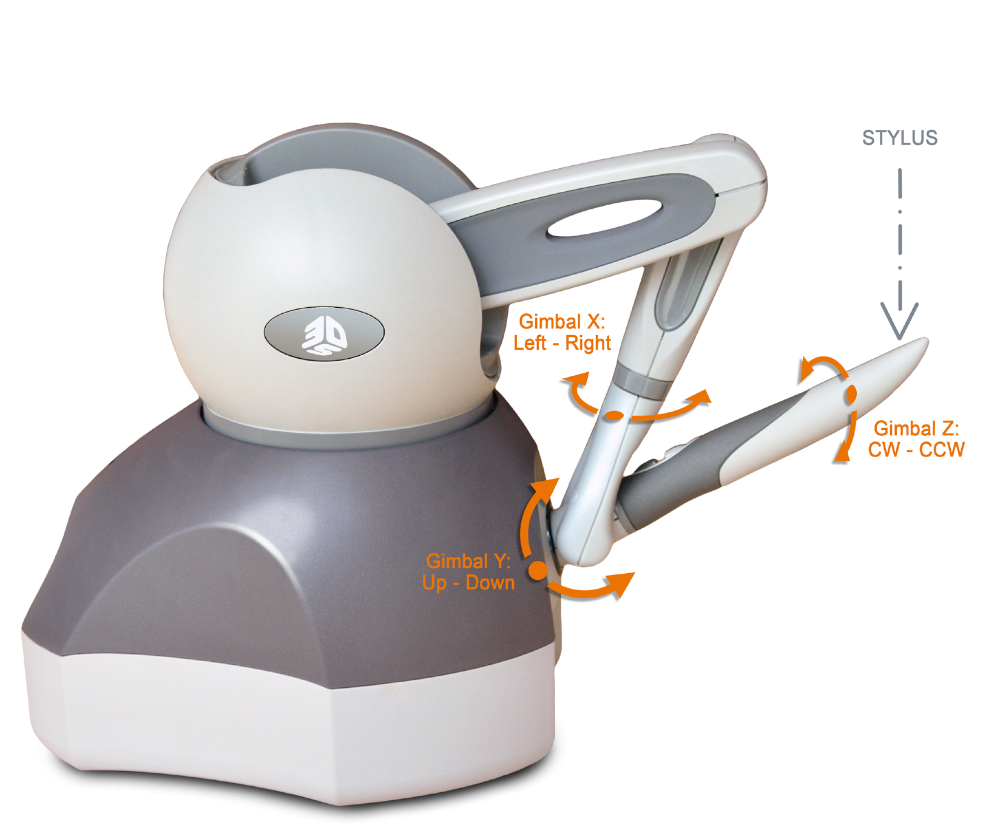
\includegraphics[width=0.48\linewidth]{integration/touch_hero_dofs}
  \caption{Different encoders and degrees of freedom for 3D Systems Touch}
  \label{fig:touch}
\end{figure}

\subsection{Stereoscopisc Rendering}
\label{ssec:stereo}
\begin{figure}
  \centering%
  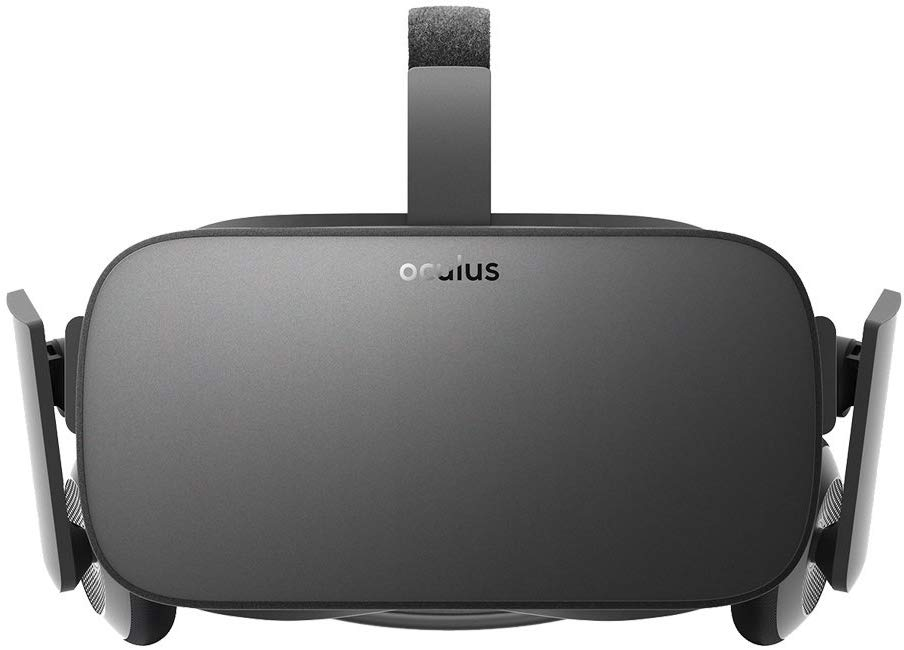
\includegraphics[width=0.45\linewidth]{integration/oculus_rift}
  \hfill%
  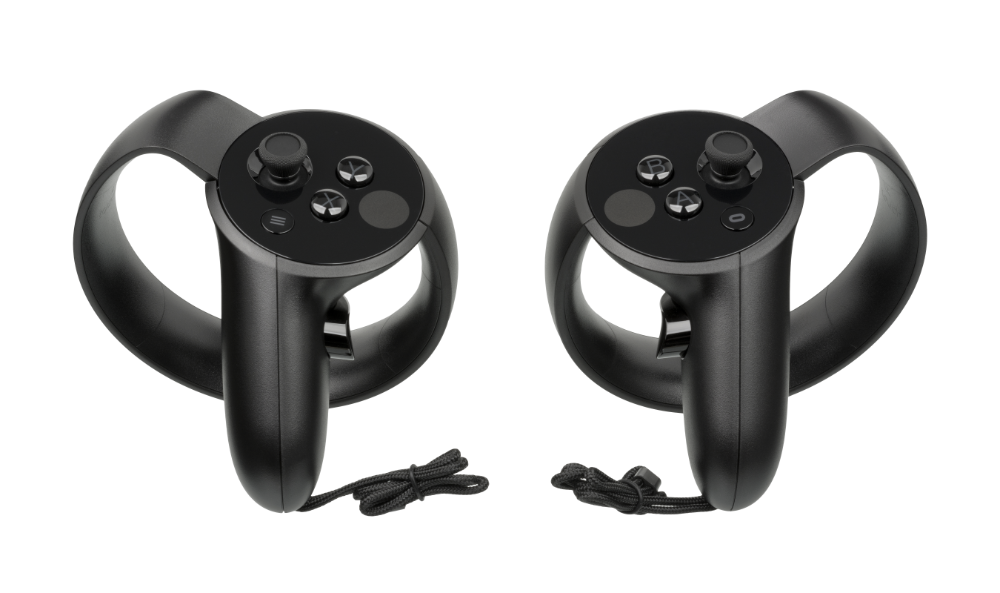
\includegraphics[width=0.54\linewidth]{integration/oculus_rift_touch}
  \caption{Oculus Rift and Oculus Touch}
  \label{fig:oculus}
\end{figure}

We've enhanced our stereoscopic rendering techniques to work better with stereo displays and we're working on extending our routines to support Oculus Rift and Touch shown in \autoref{fig:oculus} for a more immersive experience.

\hrule%

\begin{enumerate}
  \item Photo from spider interface PR \#
  \item EndoWrist kinematics slides PR 2
\end{enumerate}

\hrule%

\subsection{Cross-Platform Integration}
\label{sec:cross}

We have integrated more libraries into our CMake-based build process. Our whole system is now under one repository with centralized access to all collaborators.

\subsection{User Interface}
\label{sec:console}
To simulate a realistic presentation of a medical surgery for surgeons to train on, we need to have the same graphical interface as the real surgeries. Hence we need to mimic the graphical interface of the surgical robot in our simulation, but with the addition of feedback queues to help trainees understand their actions during the surgery.

Using a C++ graphical library that can be layered on top of our simulation, easy to use and has no extra/separate code or libraries required, and that works on all three major operating systems: Windows, macOS, and GNU/Linux). To achieve this we decided to try out two of the most popular and widely used C++ graphical user interface libraries: NanoGUI and ImGUI.

\subsubsection{NanoGUI}
\label{ssec:nanogui}
We went with NanoGUI first to assess it according to our requirements. NanoGUI is a minimalistic cross-platform widget library written in C++ for OpenGL which already meets two of the requirements. We started with testing it with our basic requirements by adding images, buttons, inputs, and drop-down menus. The widgets additions were fairly simple and looked promising for our goal, but all of the widgets were windowed, as can be seen below.

\begin{figure}
  \centering%
  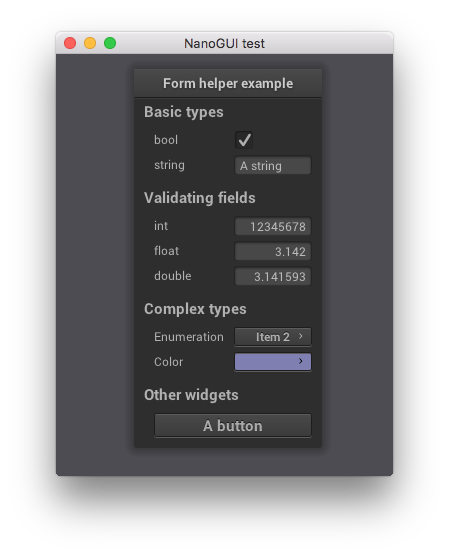
\includegraphics[width=0.5\linewidth]{integration/nanogui}
  \caption{---}
  \label{fig:}
\end{figure}

Next we went on to see if we can make the widgets translucent, especially images. We were able to control the images translucency, but when it came to the other widgets we faced our first obstacle as it wasn’t as direct as the images. For the buttons to be translucent, we had to change the theme of NanoGUI which means it takes effect on multiple widgets that share similar components and all the buttons will be translucent, which does conflict with our needs but it was not a huge issue, and we could work around it by overlaying the transparent widget over an image that act as a non transparent background color for the widget.

Now we need to meet our last requirement, removing the window and the title menu as seen in the figure above. There were no options in NanoGUI to remove them directly, so we needed to find a way to achieve that behaviour. We started with trying to make the title menu completely transparent but with no luck, and same goes for the background of the window. After multiple attempts we managed to bring the widget to the front of both the window and title menu, then resize them to the widget dimensions to make it the only thing visible, as can be seen below with one button. This worked for buttons, text, and inputs, but not for drop-down menus and images. For drop-down menus when clicked on, the dropdown does not show because of the size of the window, while for images, when we make them translucent, the window and title menu show, which is a deal breaker as it violates two of the crucial requirements.

\begin{figure}
  \centering%
  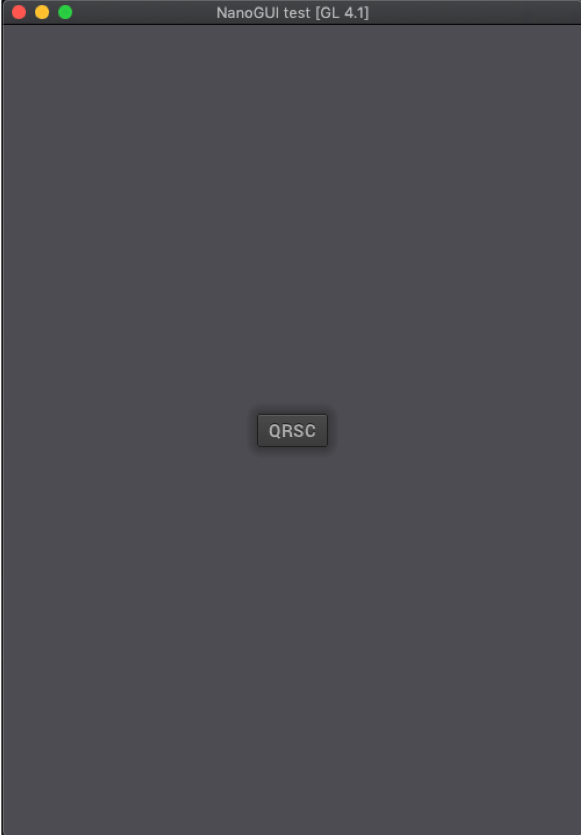
\includegraphics[width=0.4\linewidth]{integration/cropped_button}
  \caption{---}
  \label{fig:}
\end{figure}

In conclusion, given the behaviour of NanoGUI and the requirements it both met and did not meet, and in addition to the complexity of overcoming some constraints, we marked NanoGUI as an unsuitable tool for this project and other future projects.

\subsubsection{ImGUI}
\label{ssec:imgui}
After deciding on NanoGUI not being a good fit, we moved on to our second option ImGUI. ImGUI is a light-weight graphical user interface library for C++ that is fast, portable, renderer agnostic, and self-contained (no external dependencies). So just like NanoGUI, ImGUI is both written in C++ and cross-platform making it easier for us to integrate it with our simulator. We first started testing ImGUI with removing the window and the title menu, and we managed to do that with only two lines of code, which was a big improvement from NanoGUI both in simplicity and functionality, in addition to controlling the resizing and the movability of the window. After it, we added widgets which had a better structure in the form adding them to our \acr{gui}, where each widget such as buttons and labels had their own styling properties that can be applied. In addition, we were able to add images, make them translucent and overlay text on top of them as shown below. Given that, ImGUI met all our requirements, this gave us the green light to go ahead and use it for our graphical interface.

\begin{figure}
  \centering%
  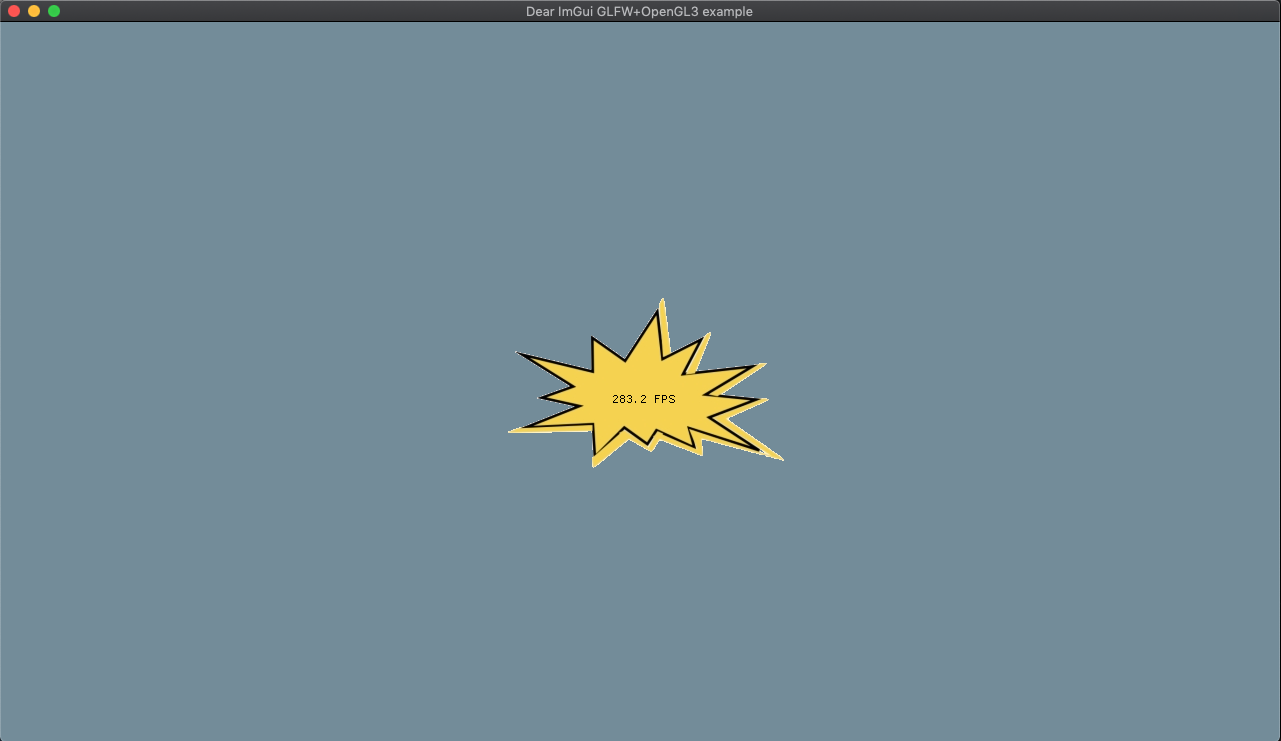
\includegraphics[width=\linewidth]{integration/imgui}
  \caption{---}
  \label{fig:}
\end{figure}

\subsubsection{Graphical User Interface}
\label{ssec:gui}
We started creating our \acr{gui} by looking at the \acr{gui} of the da Vinci Robot that is used in the surgeries we are working on simulating for surgeons to train on.

Given these images, we started recreating the widgets in sketch to have them in high resolution to look crisp on all sizes of monitors. In addition, we used our own fonts for the text to give an elegant and simple design to the \acr{gui}, especially in the feedback dialogs for the trainees, making it easy for them to read and gentle on their eyes.

\begin{figure}
  \centering%
  \setlength{\fboxsep}{0pt}%
  \setlength{\fboxrule}{0.1pt}%
  \fbox{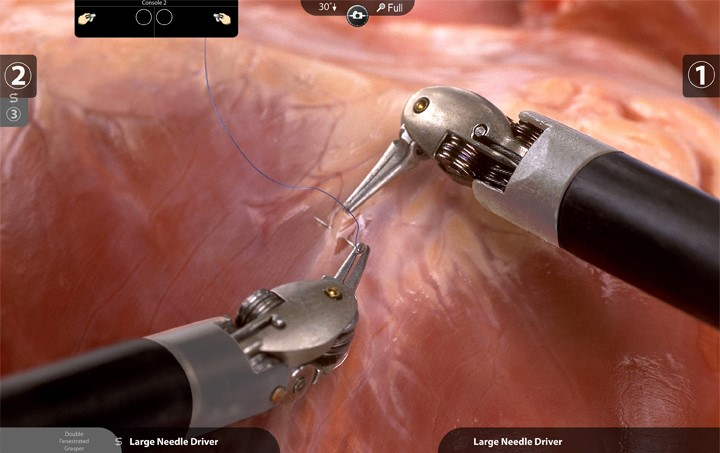
\includegraphics[width=\linewidth]{integration/davinci_snapshot}}\\[1ex]
  \fbox{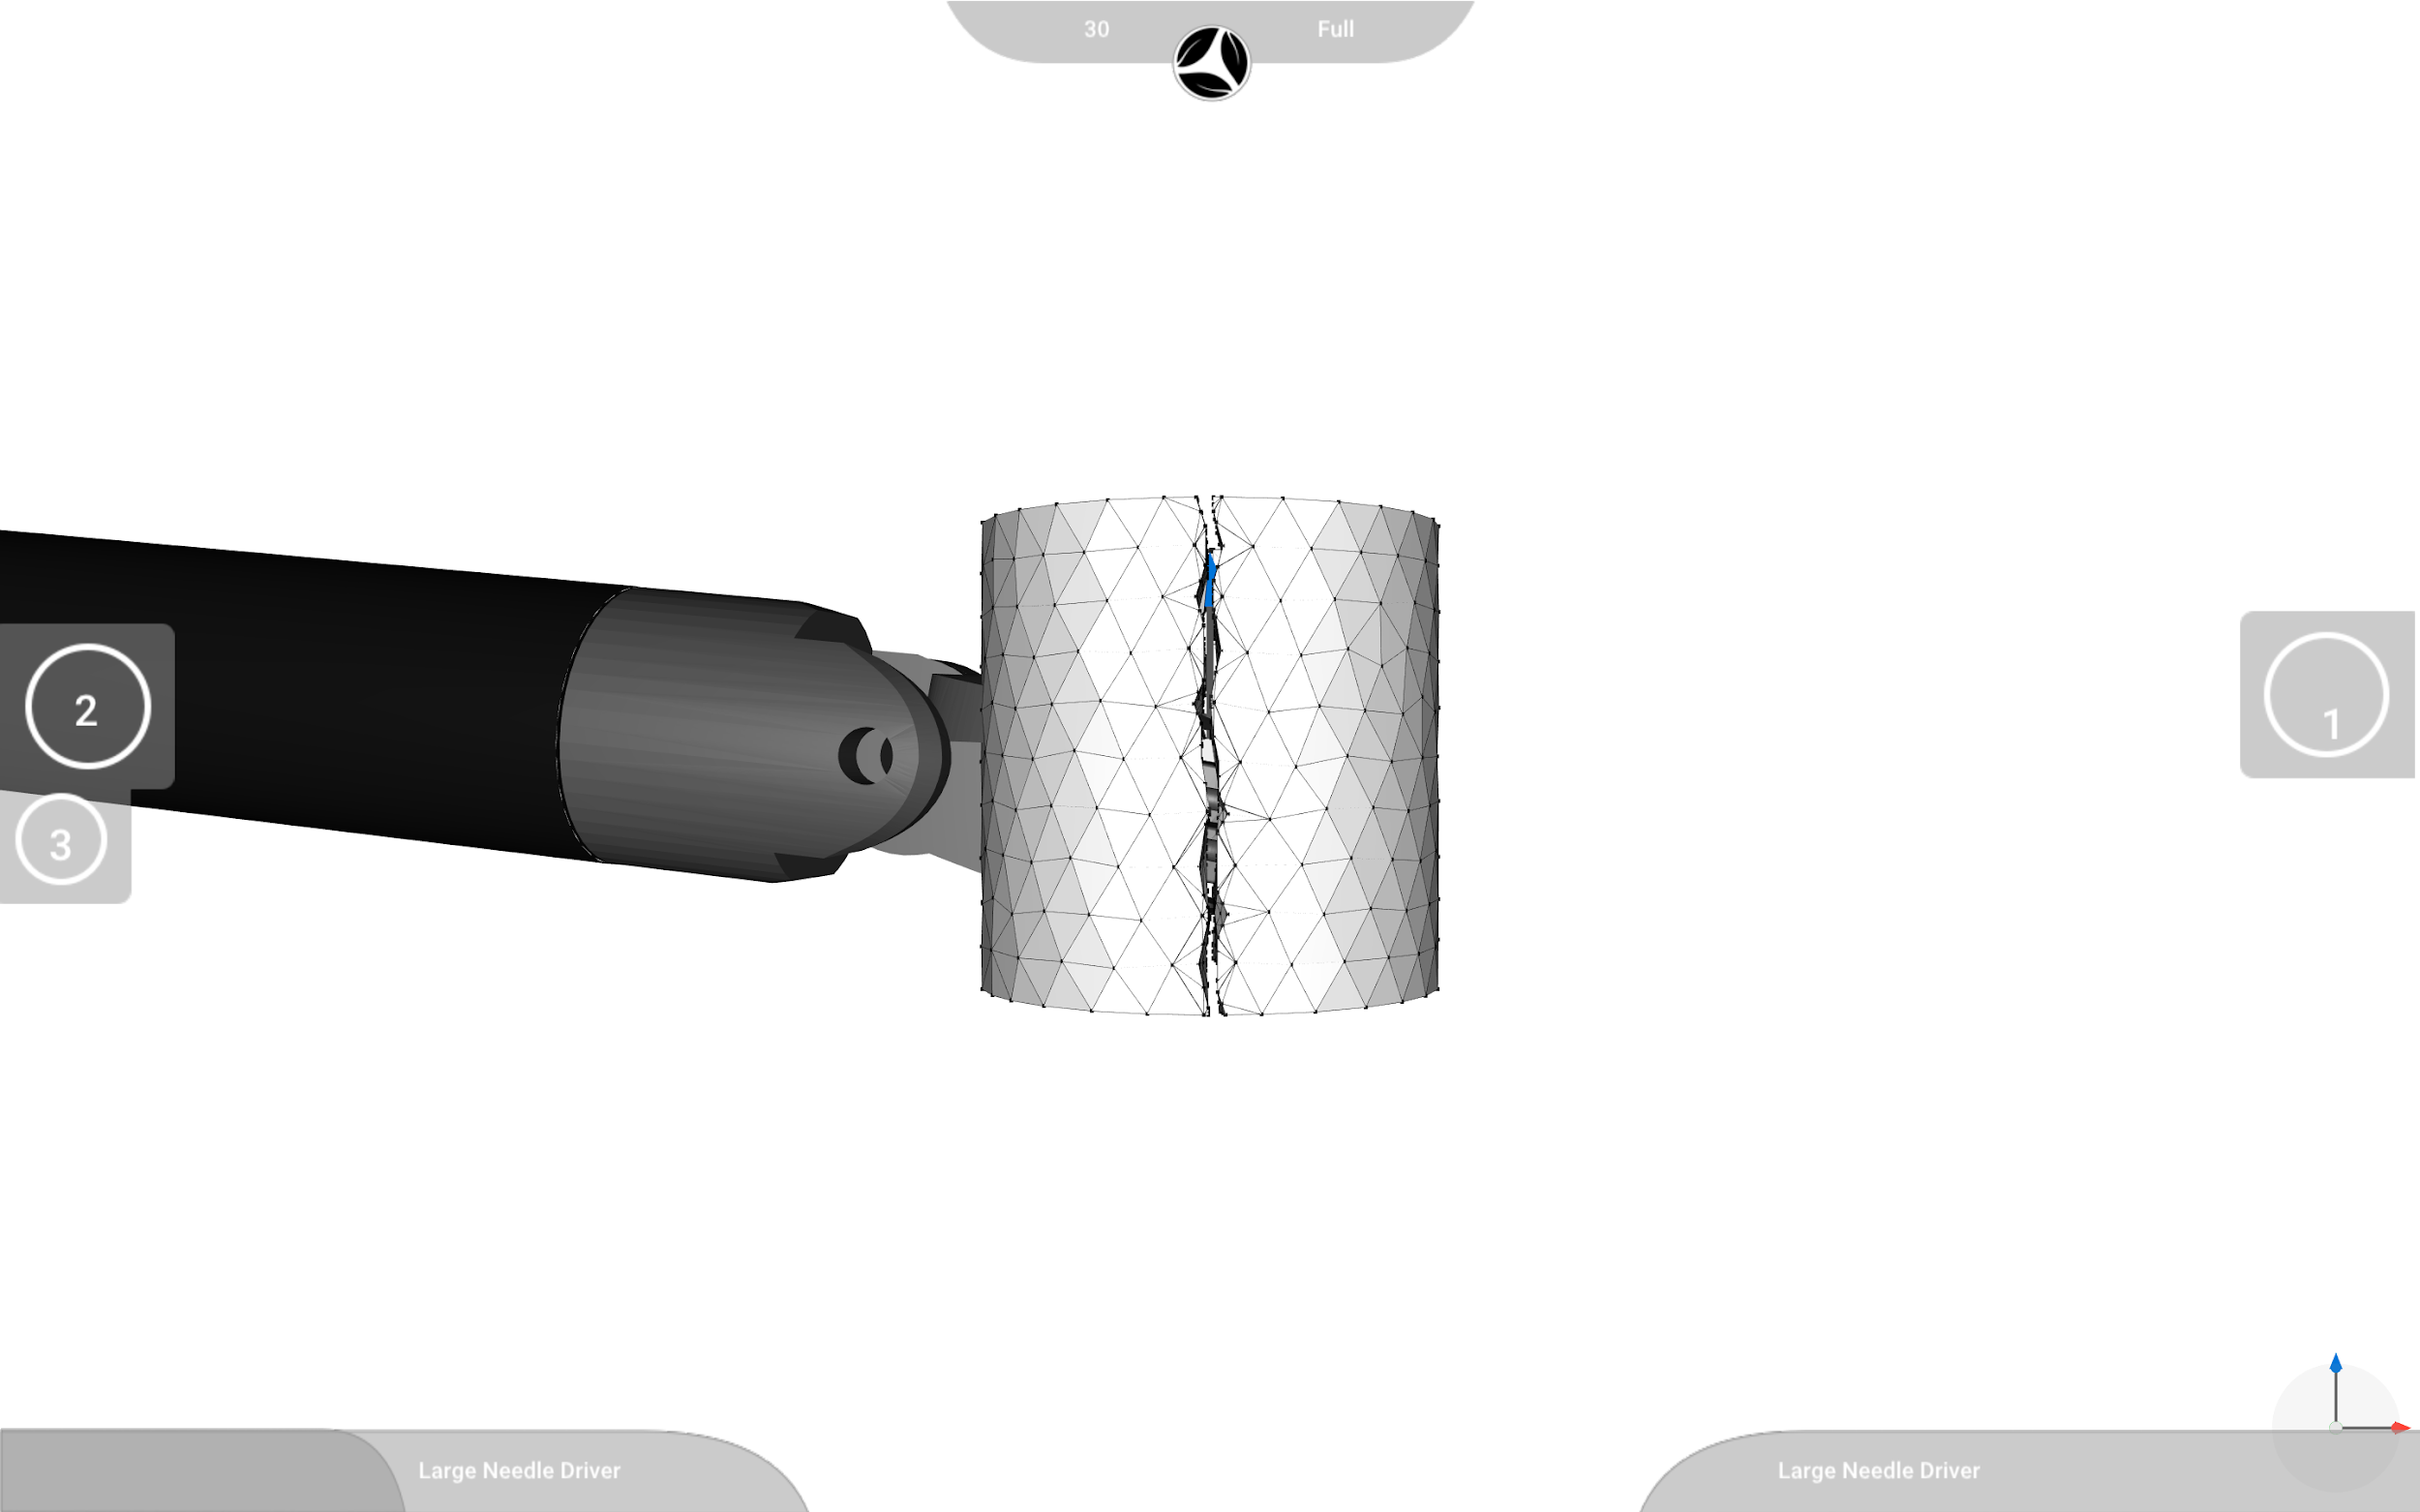
\includegraphics[width=\linewidth]{integration/interface_basic_scind}}
  \caption{---}
  \label{fig:}
\end{figure}

Following this we decided to add a popup window that allows the user to specify options and settings of the scene, in addition to adding a file dialog window, that in the future would give the user the ability to add their own scenes or models to the simulation.

\begin{figure}
    \centering%
    \setlength{\fboxsep}{0pt}%
    \setlength{\fboxrule}{0.1pt}%
    \fbox{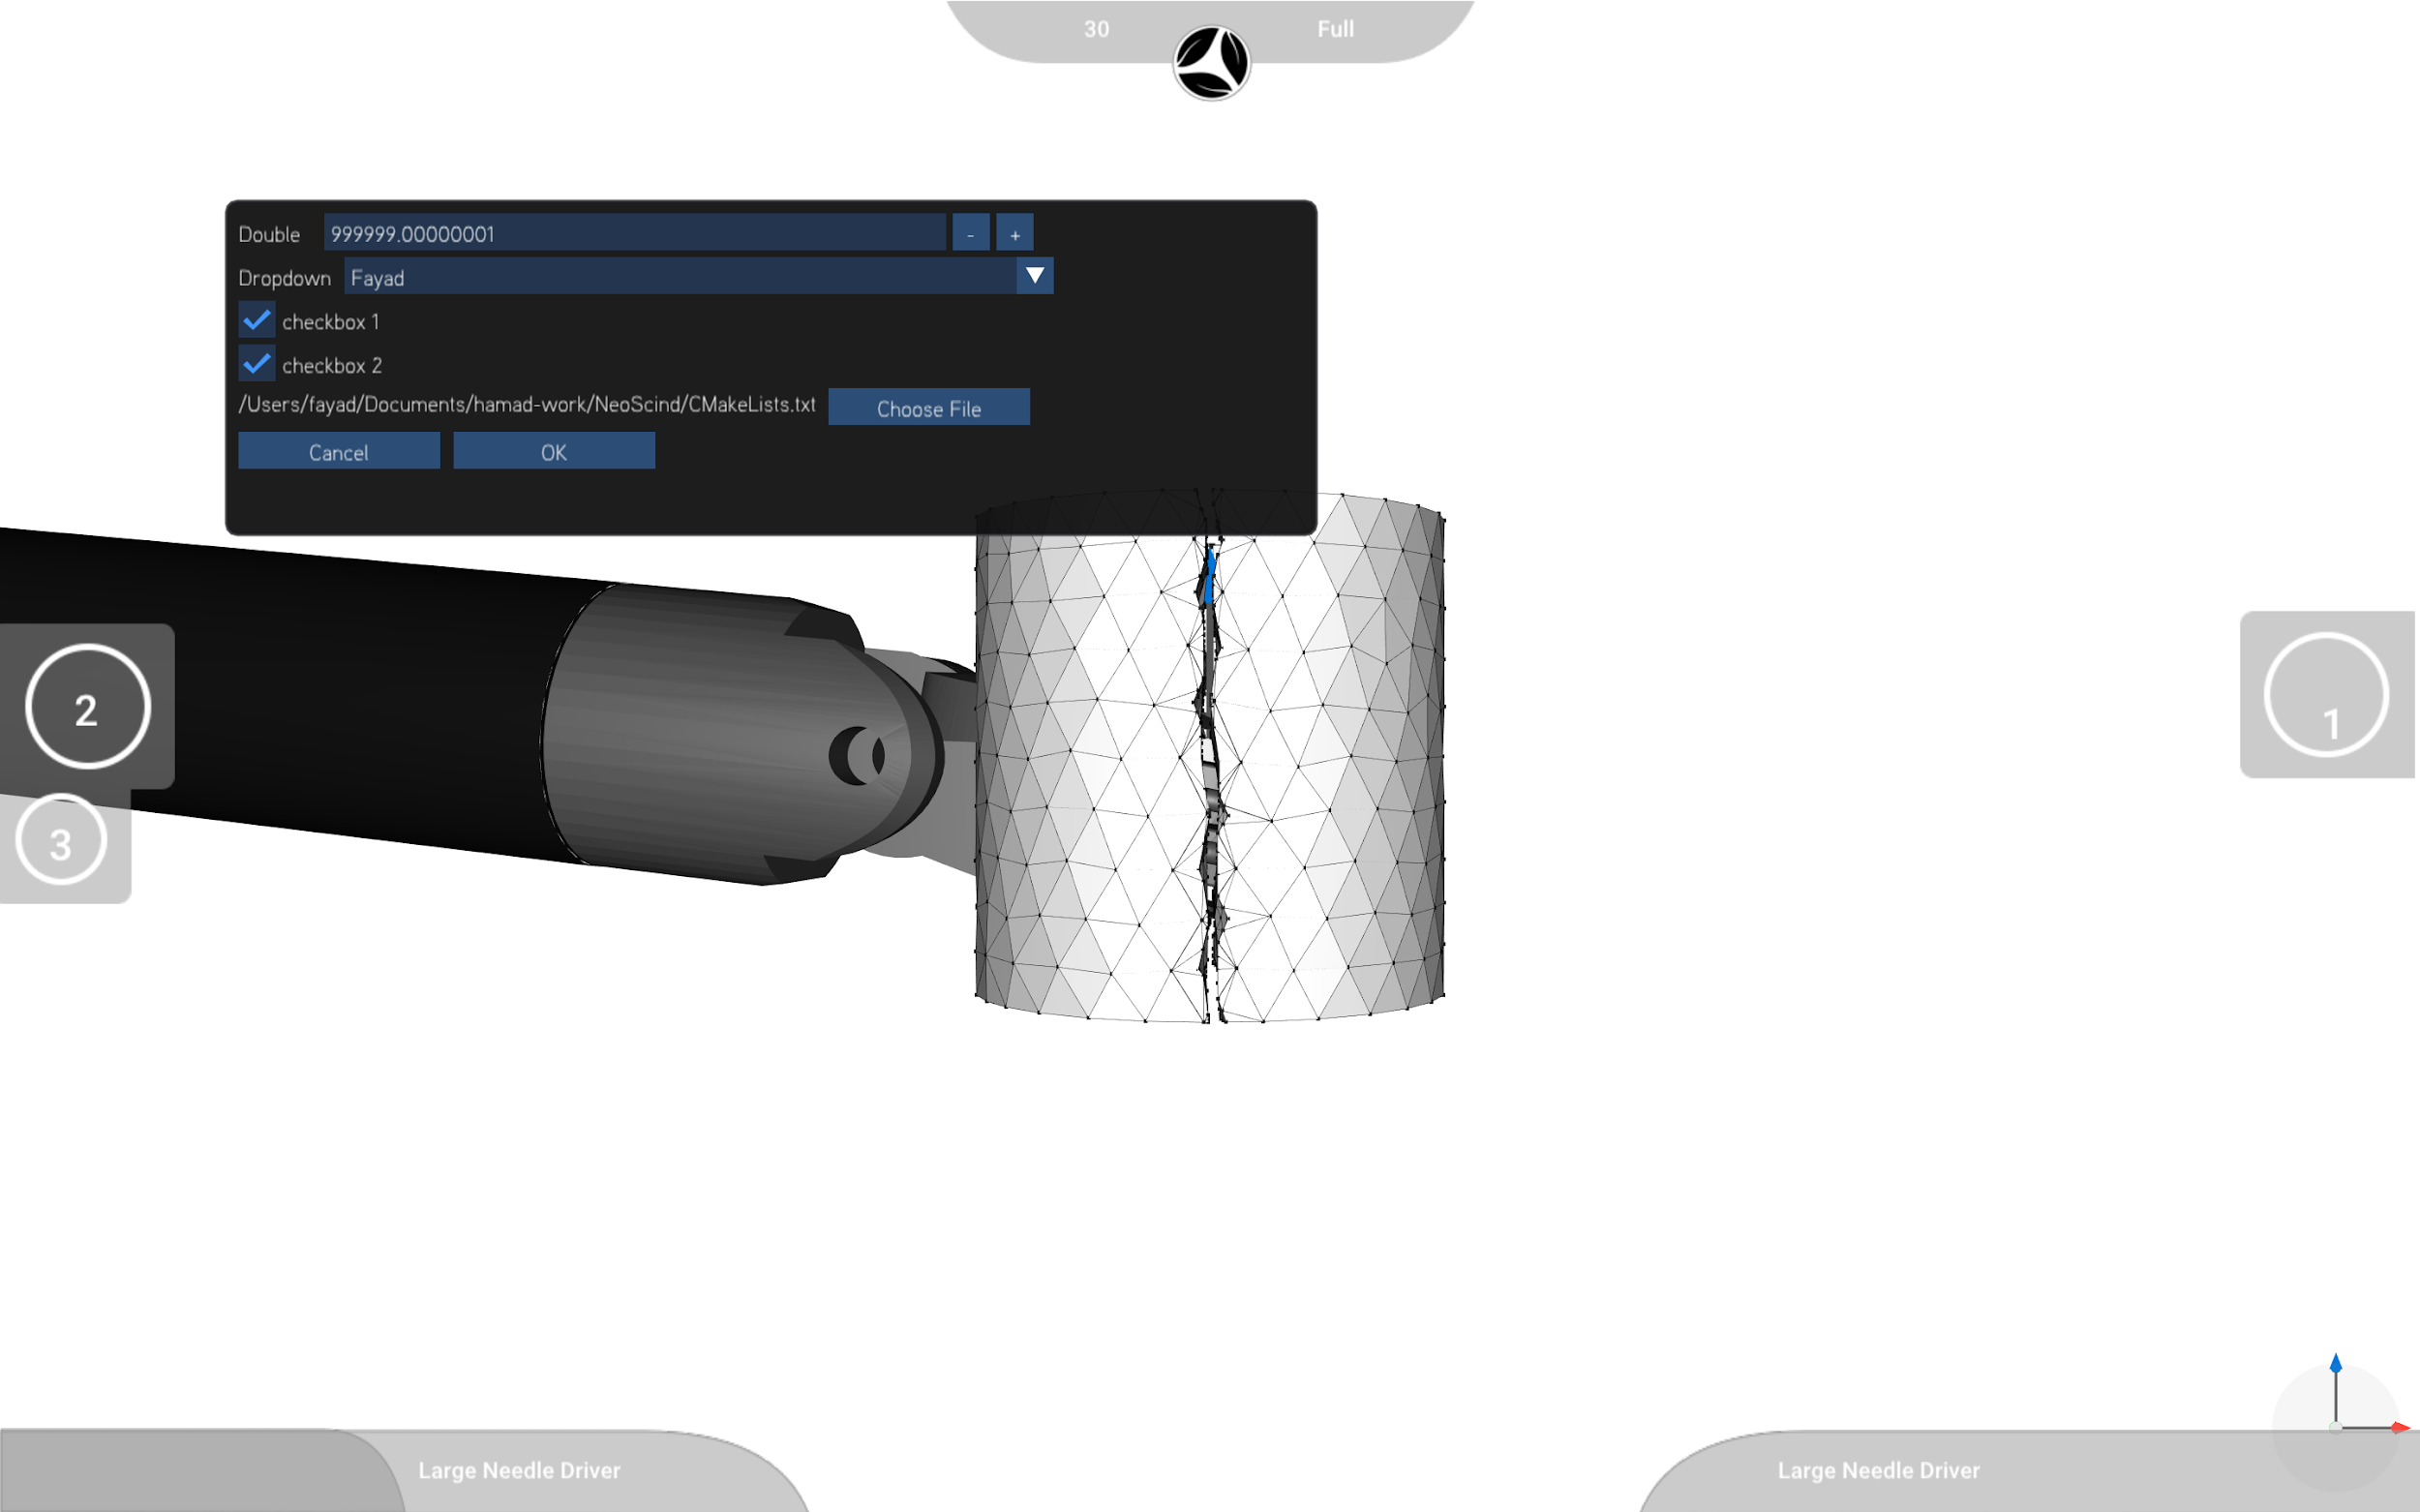
\includegraphics[width=\linewidth]{integration/interface_basic_scind_popup}}
    \caption{---}
\end{figure}

Finally, we changed the \acr{gui} to match the newest da Vinci robot (da Vinci Xi) with the addition of feedback dialogs. The purpose of this is to replicate the feel of real surgeries, so there is a smooth transition when the trainees transition from our simulator to the da Vinci Xi, in addition to giving them feedback on their progress to reinforce learning the right techniques, by giving them a good explanation of why their actions were not ideal in that scenario and the way to correct them.

\begin{center}
  \setlength{\fboxsep}{0pt}%
  \setlength{\fboxrule}{0.1pt}%
  \fbox{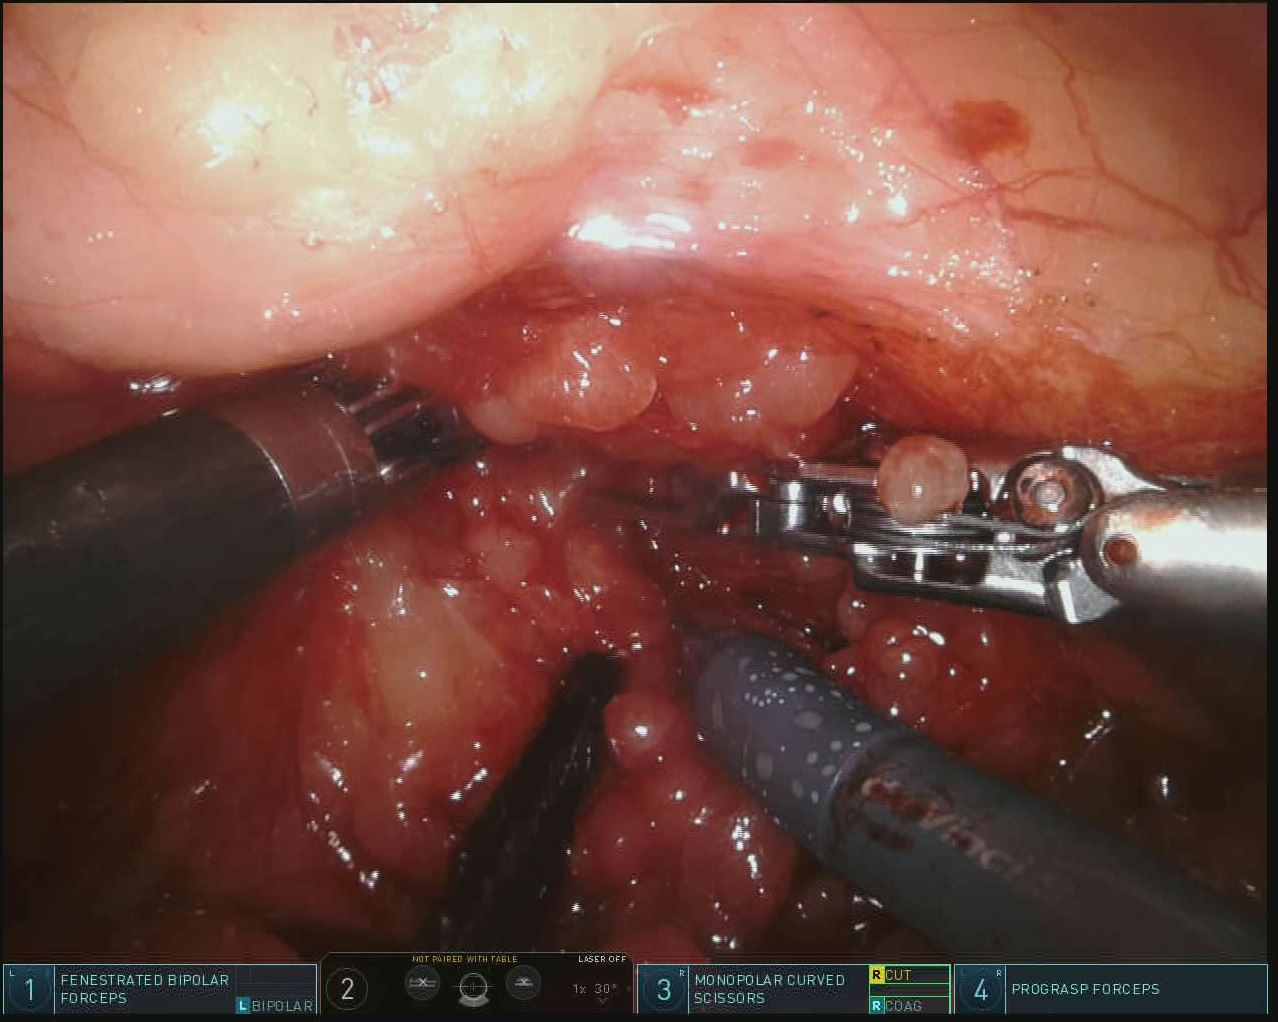
\includegraphics[width=\linewidth]{integration/davinci_xi}}
\end{center}

In conclusion, NanoGUI appeared to be less flexible than ImGUI, giving ImGUI the advantage for us to use it in this project and future projects. Furthermore, we managed to recreate the da Vinci robot \acr{gui} to have a simulation that resembles the real feel of surgeries as much as possible, at least when it comes to the graphical interface.

\begin{figure}
  \centering%
  \setlength{\fboxsep}{0pt}%
  \setlength{\fboxrule}{0.1pt}%
  \fbox{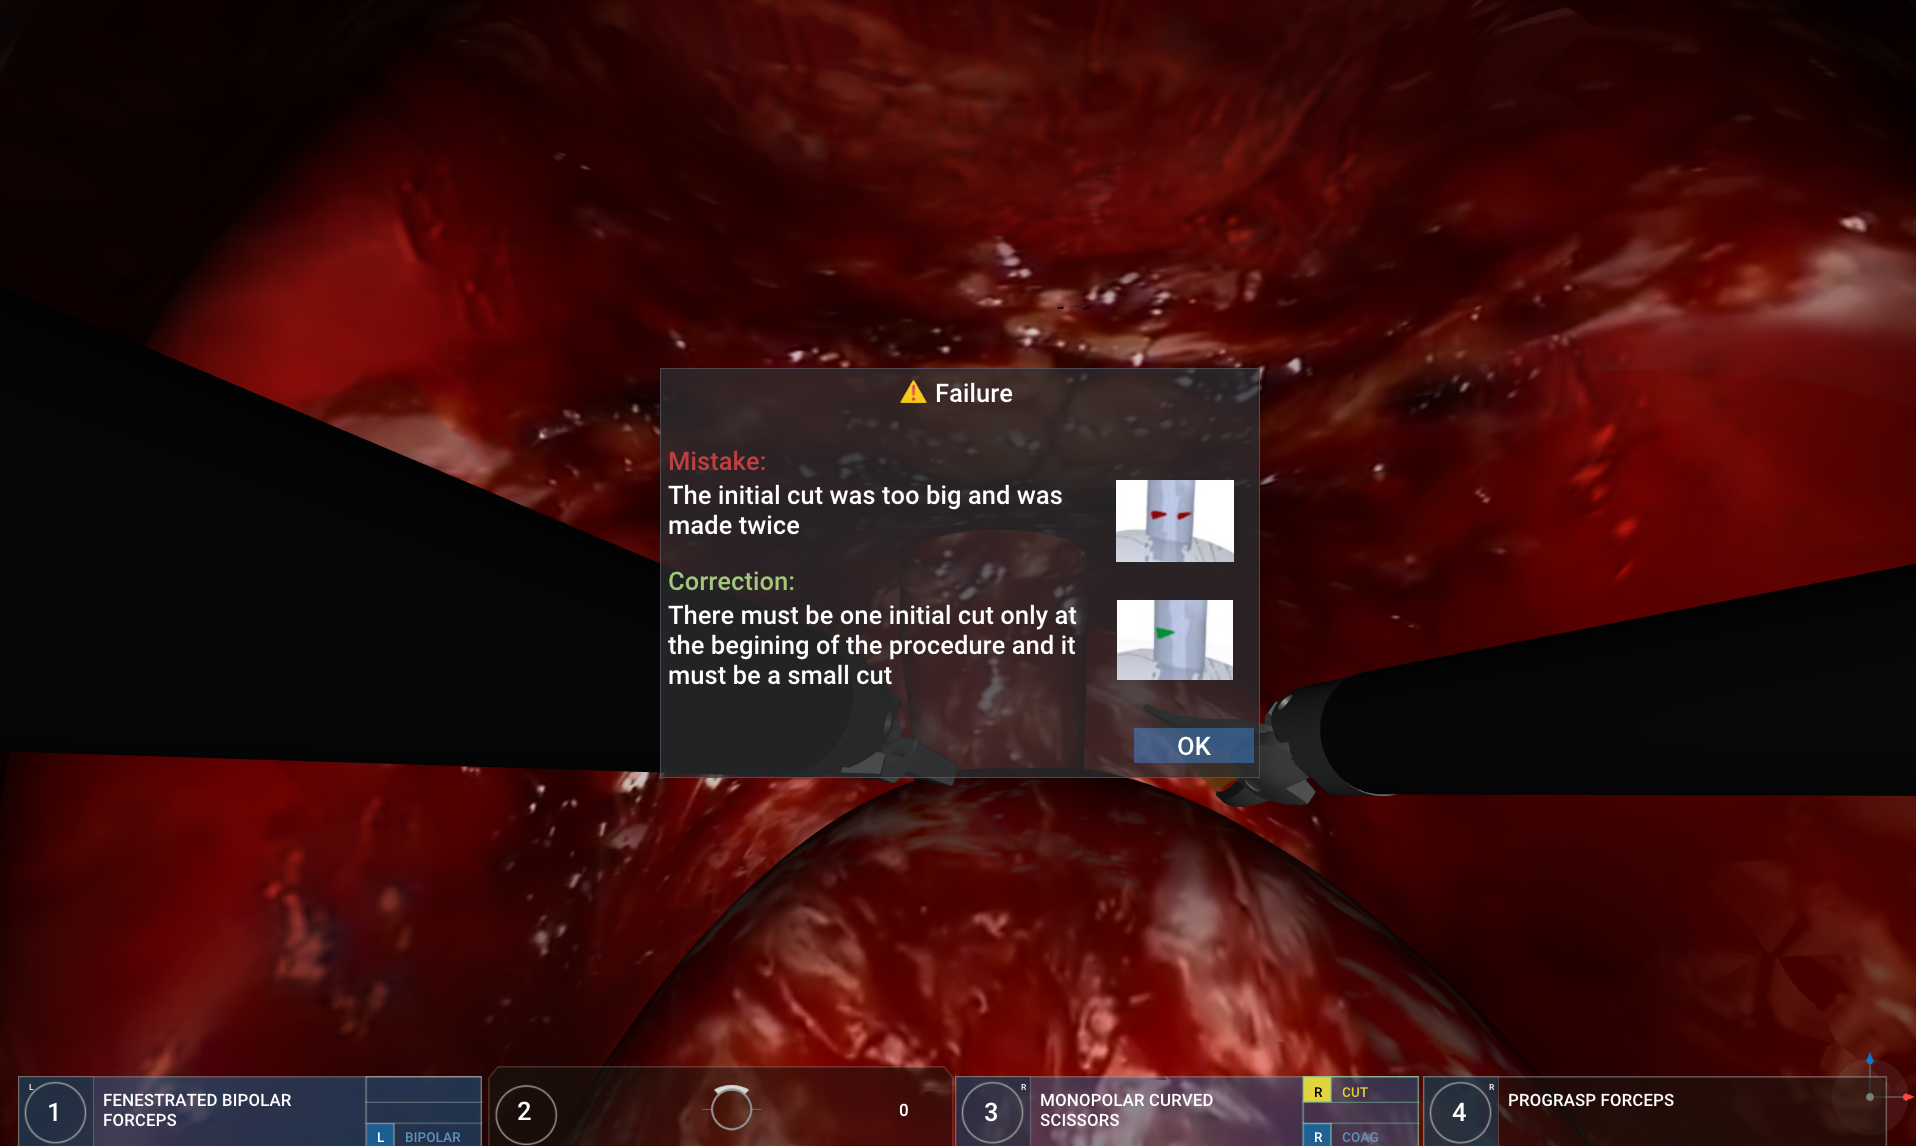
\includegraphics[width=\linewidth]{integration/interface_scind}}\\[1ex]
  \fbox{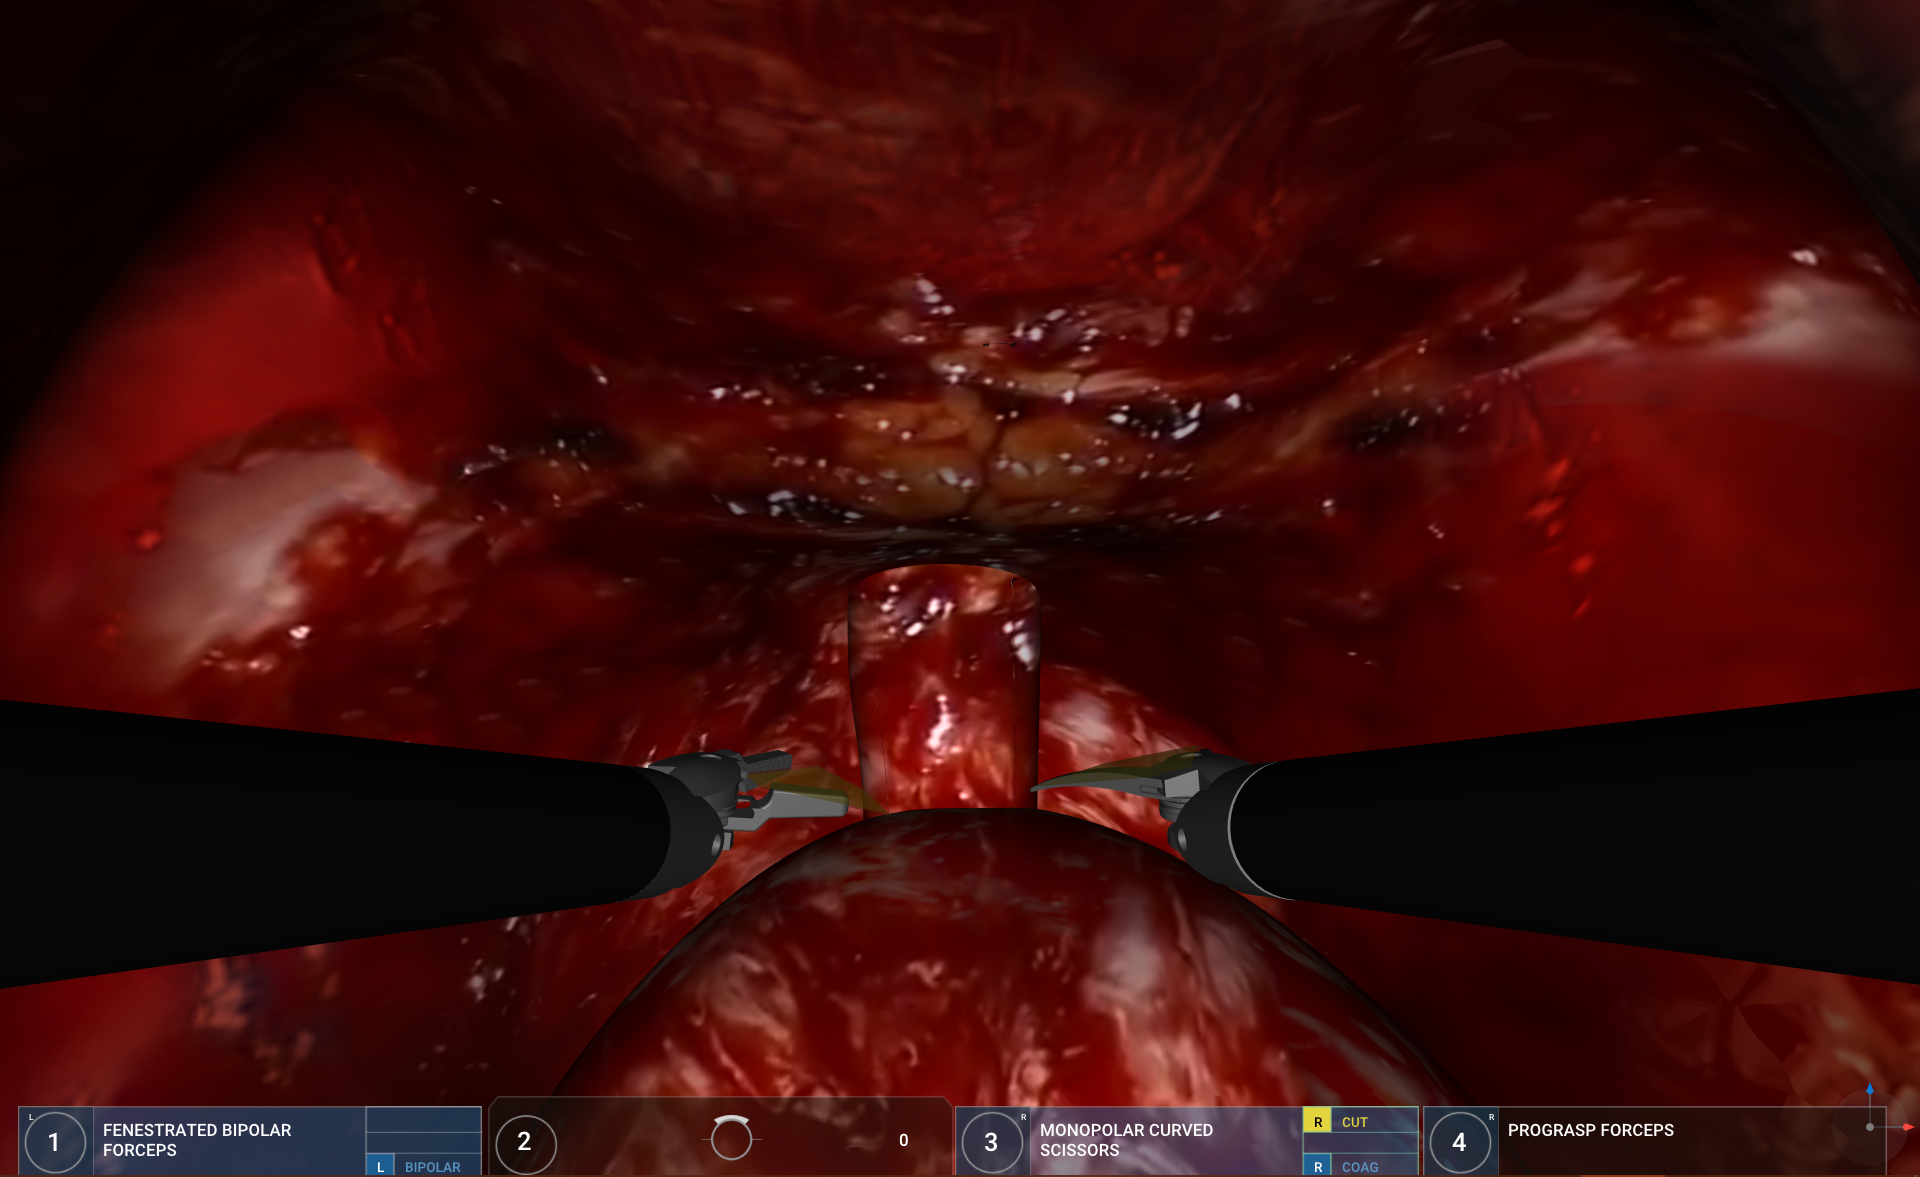
\includegraphics[width=\linewidth]{integration/interface_scind_popup}}
  \caption{---}
  \label{fig:}
\end{figure}

%\section{Haptic Control}\label{sec:haptic}

%\section{Stereoscopic Rendering}\label{sec:stereo}

\subsection{SOFA}
\label{sec:sofa}
We want to create a robotic surgery simulator similar to what we are making but in using the available solutions that exist to have a comparison to evaluate and measure our solution performance to them.

Using SOFA framework as a tool to develop the robotic surgery simulation. SOFA is an efficient framework dedicated to research, prototyping and development of physics-based simulations that is both open source and cross-platform, this gives the ability to use it freely and modify it on the same three platforms we work on. We wanted to use SOFA since it is extensively used in medical simulation and is mature enough for development since it is been around since 2005.

We want to do the following tasks in SOFA:
\begin{enumerate}[1.]
  \item Loading of both surface and volumetric 3D models (VTK, OBJ, STL, and other),
  \item Deformation of 3D models,
  \item Cutting of 3D models, and
  \item Using the omni phantom as a user input interface.
\end{enumerate}

\subsubsection{Loading 3D models}
We want to be able to load 3D models to apply the other functions we need. Loading both volumetric and surface 3D models in SOFA was fairly straightforward. Next step, was adding textures to these models, and rendering them was a built-in function.

\begin{figure}
  \centering%
  \setlength{\fboxsep}{0pt}%
  \setlength{\fboxrule}{0.1pt}%
  \fbox{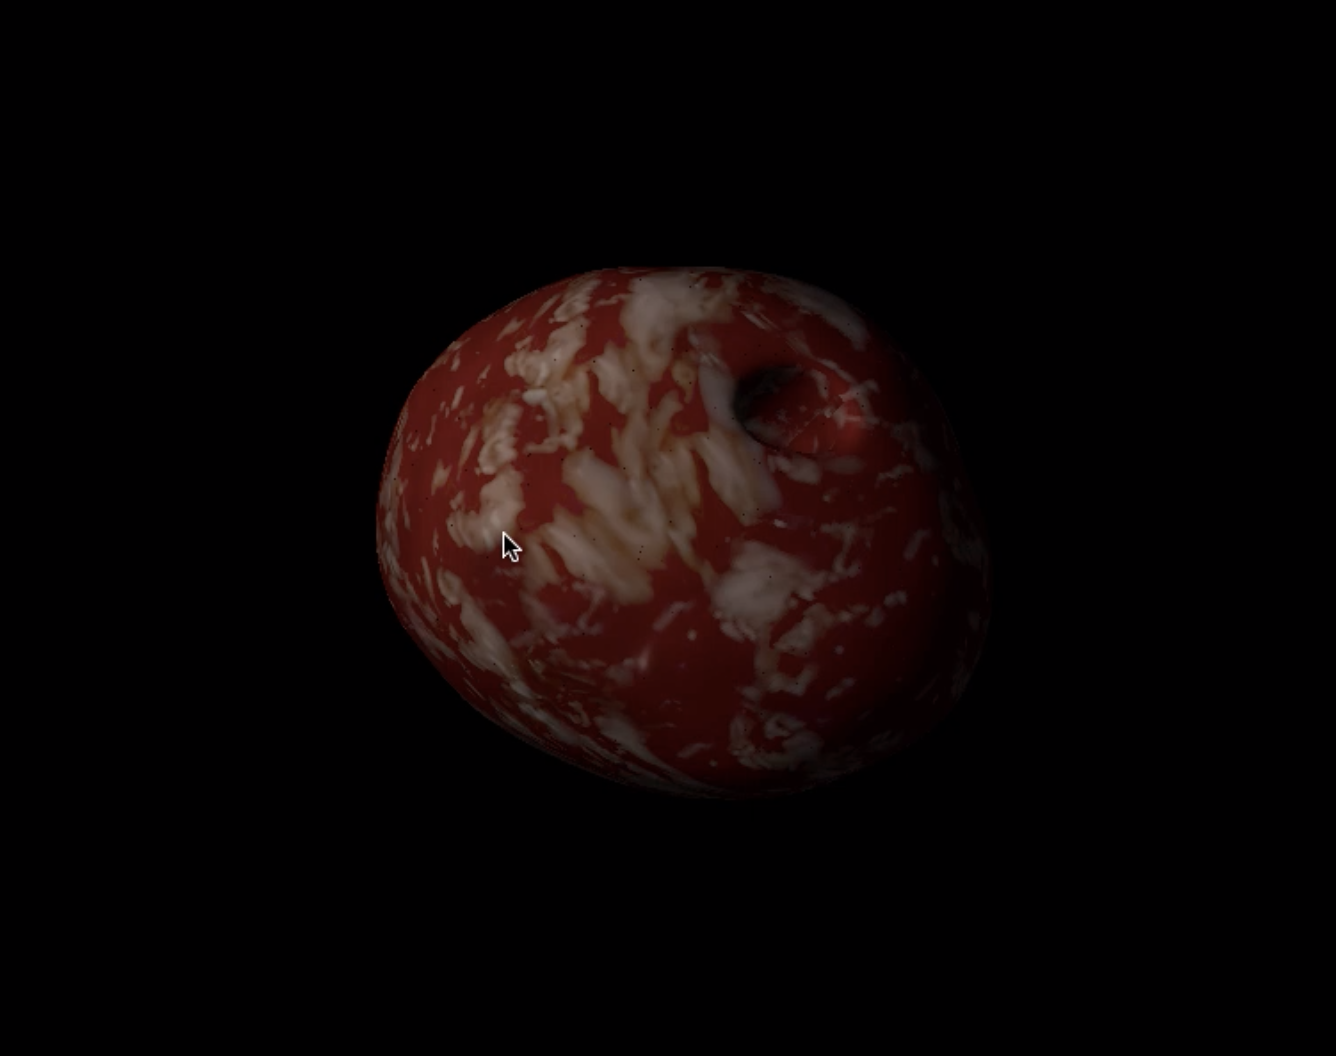
\includegraphics[width=0.7\linewidth]{integration/sofa_textures}}
  \caption{---}
  \label{fig:sofa_textures}
\end{figure}

\subsection{Deformation}
Next step was us looking at the physics of the engine, specifically the deformation. SOFA provided multiple types for the model to take, Rigid, Vec3, Vec6. The Vec3 type give us the deformable behaviour we want, which is added to the model in the loading part by changing the template. In addition, we used the rigid body template for the scissors as they need not to deform on impact.

\begin{figure}
  \centering%
  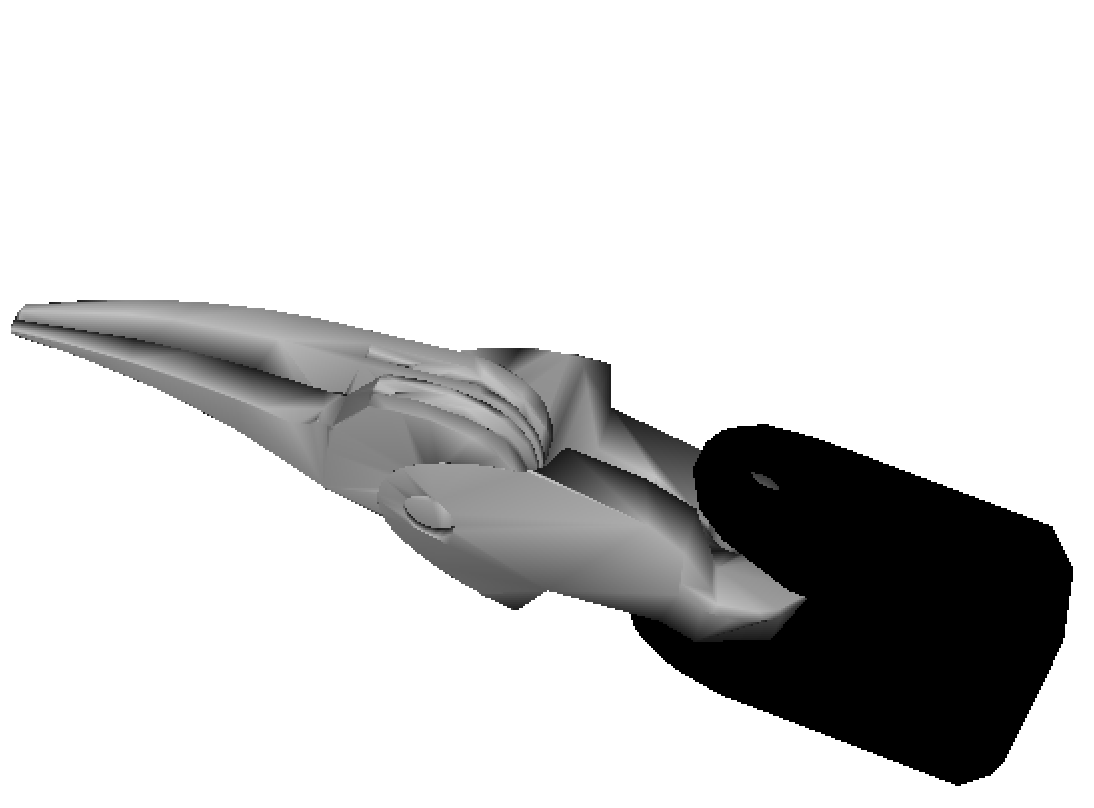
\includegraphics[width=0.35\linewidth]{integration/sofa_endowrist}
  \caption{---}
  \label{fig:sofa_endowrist}
\end{figure}

\subsubsection{Cutting}
Now we want to implement the cutting to simulate the dissection in a robotic surgery. To achieve this we had to use a SOFA plugin called SOFA Carving Plugin, which gave us the capability to cut a 3D mesh. The cutting was not as advanced as our cutting algorithm, instead it was doing the more basic and traditional way of cutting, which was simply deleting triangles and tetrahedra. We faced issues regarding the cutting in the scene that SOFA was limiting us to be only cutting one model, instead of multiple models, at the same time. In addition, the cutting tool was also limited to one model.

\begin{figure}
  \centering%
  
\includegraphics[width=0.35\linewidth]{integration/sofa_cloth}
  \caption{---}
  \label{fig:sofa_cloth}
\end{figure}

\subsection{Input Interface}
Finally, we worked on integrating the 3DSystems Touch with our SOFA program using another SOFA plugin. We first started with linking keyboard inputs through Python since SOFA allows the use of Python scripts to interact with its environment. Afterwards, we used a plugin provided by SOFA called Geomagic which is the same company that (used) to make the 3DSystem Touch (Omni Phantom) but it is developed by the SOFA team. The plugin gave us the capability of connecting the Touch to SOFA and moving the models using it.

\begin{figure}
  \centering%
  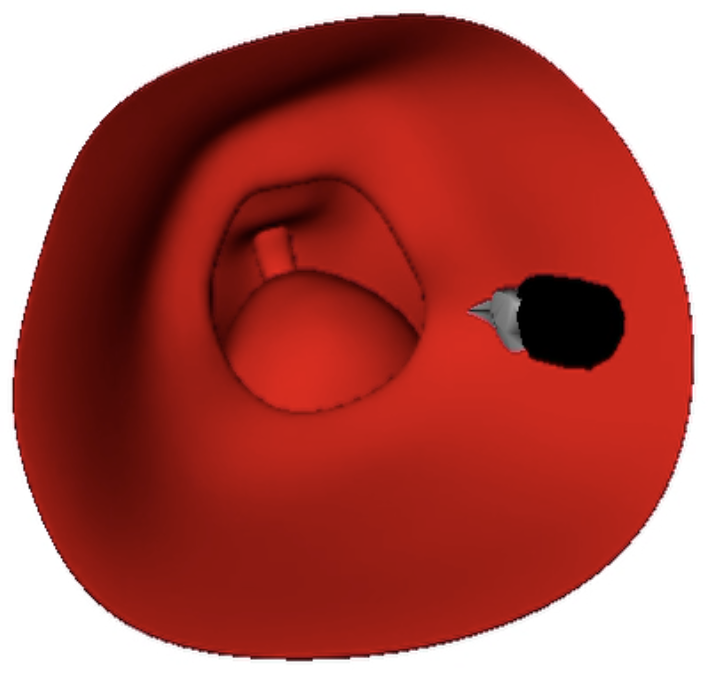
\includegraphics[width=0.5\linewidth]{integration/sofa_interaction}
  \caption{---}
  \label{fig:sofa_interaction}
\end{figure}

In conclusion, SOFA turned out to be a great choice for us to go with, given all its functionality, but it still has it is own hurdles which we need to work around.

\subsection{Scenarios Replay}
\label{sec:replay}
Our logging module that was mainly developed for Aim 5 and 6, allows us to record the user's actions and replay them. This can be used to recored multiple scenarios and to monitor a user's progress.


\begin{figure}
  \centering%
  \setlength{\fboxsep}{0pt}%
  \setlength{\fboxrule}{0.1pt}%
  \fbox{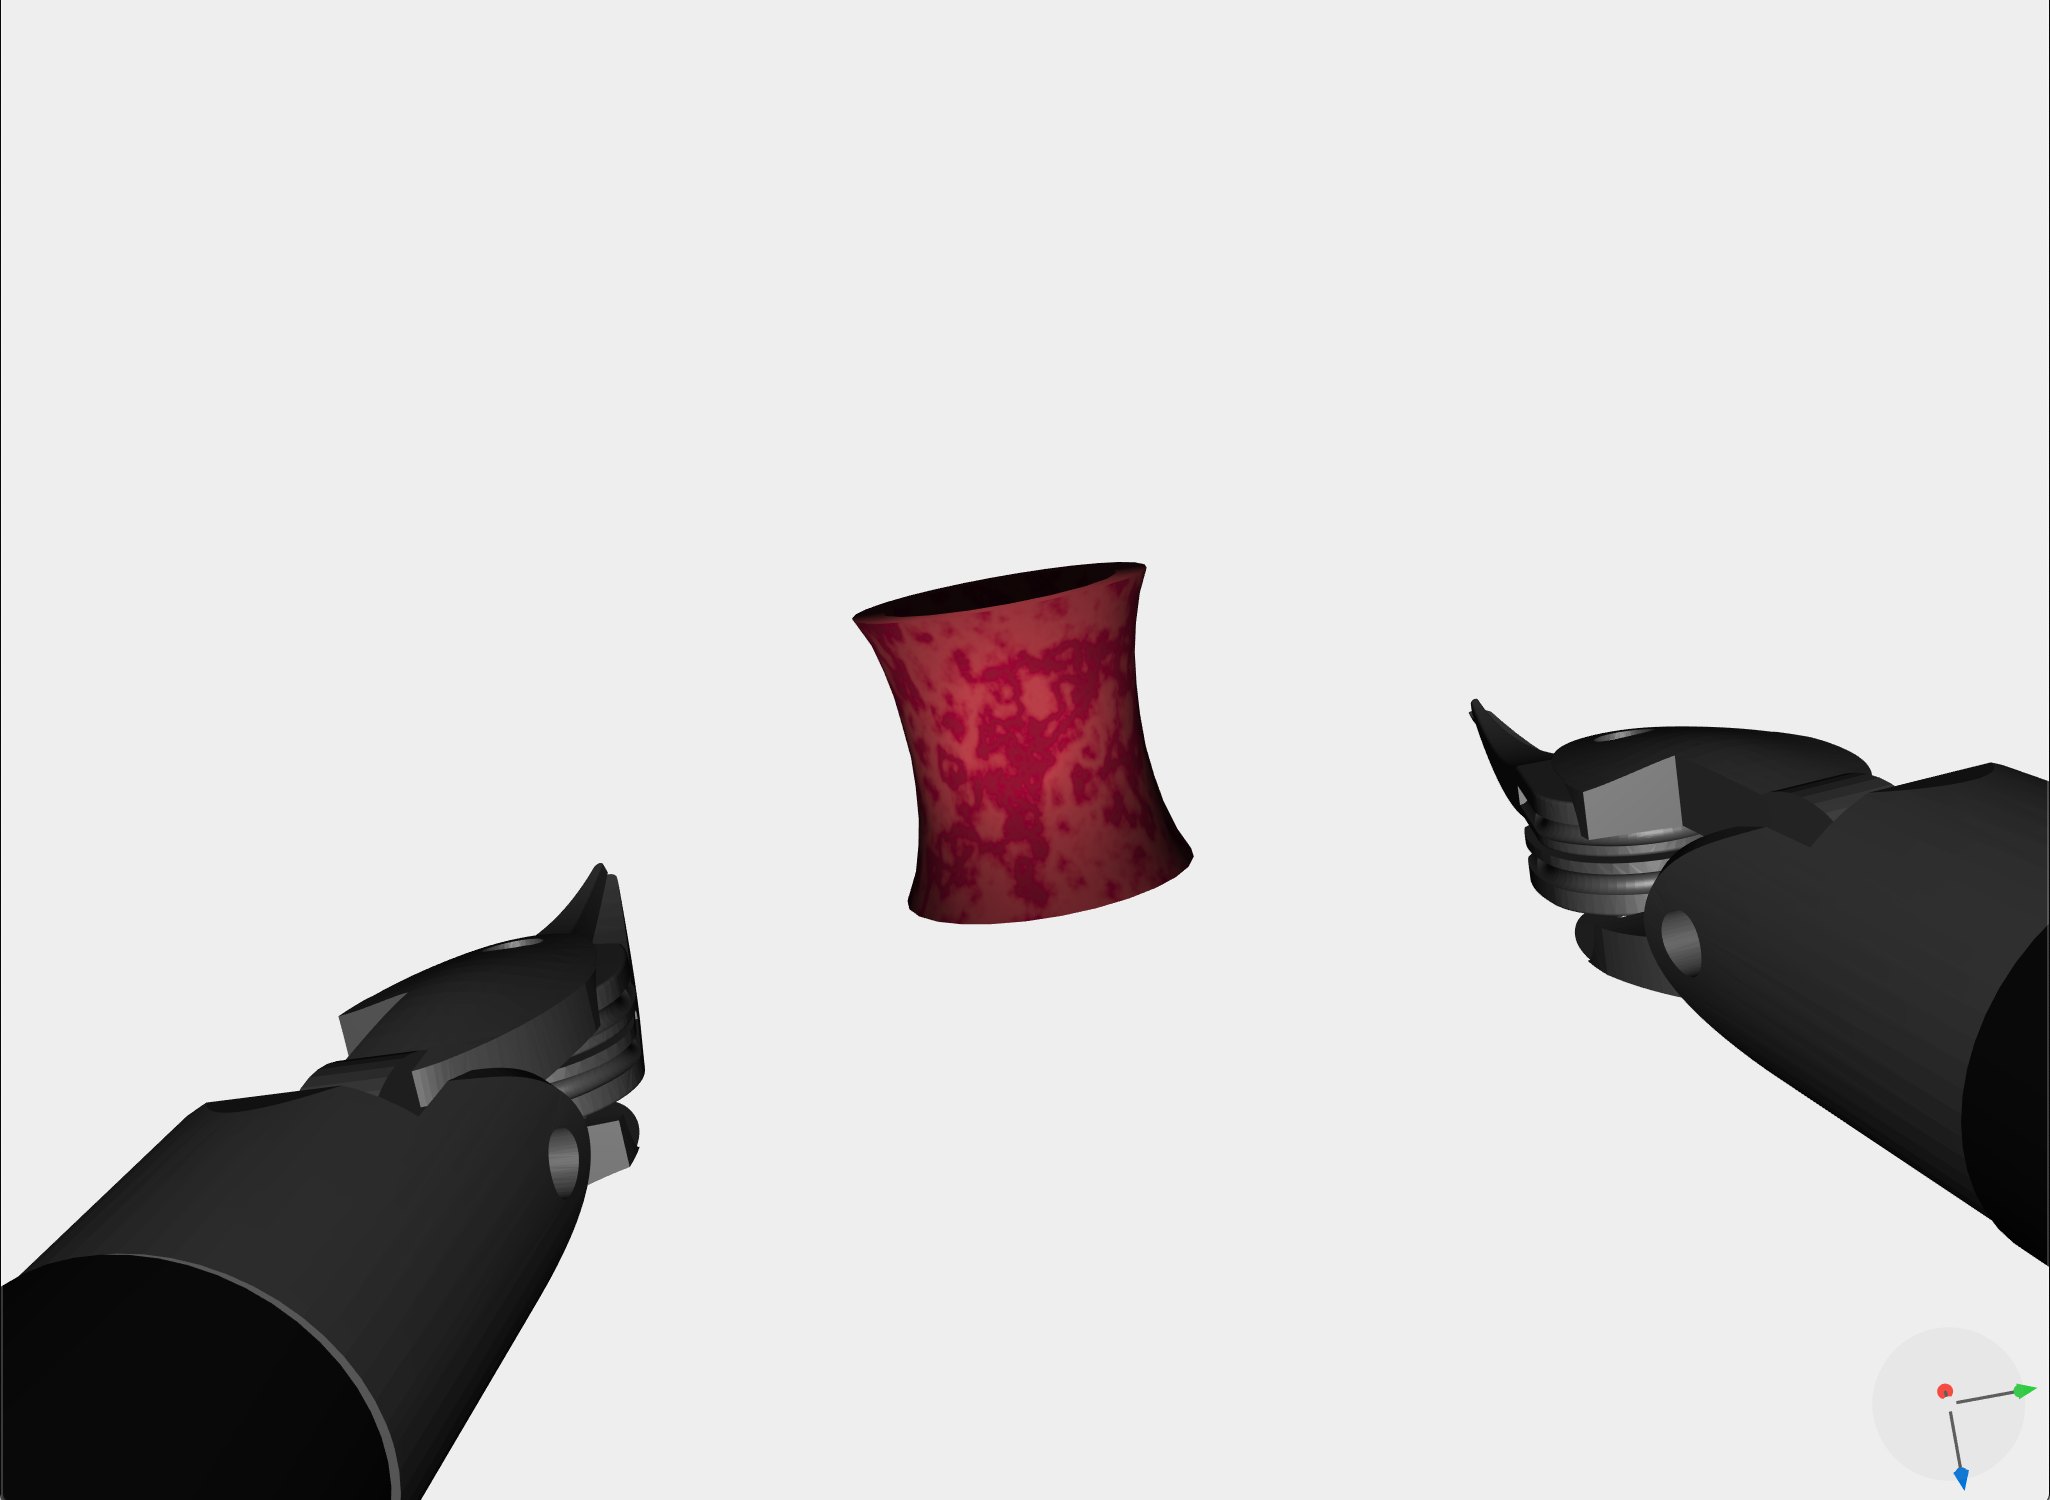
\includegraphics[width=0.49\linewidth]{integration/snap0}}\hfill%
  \fbox{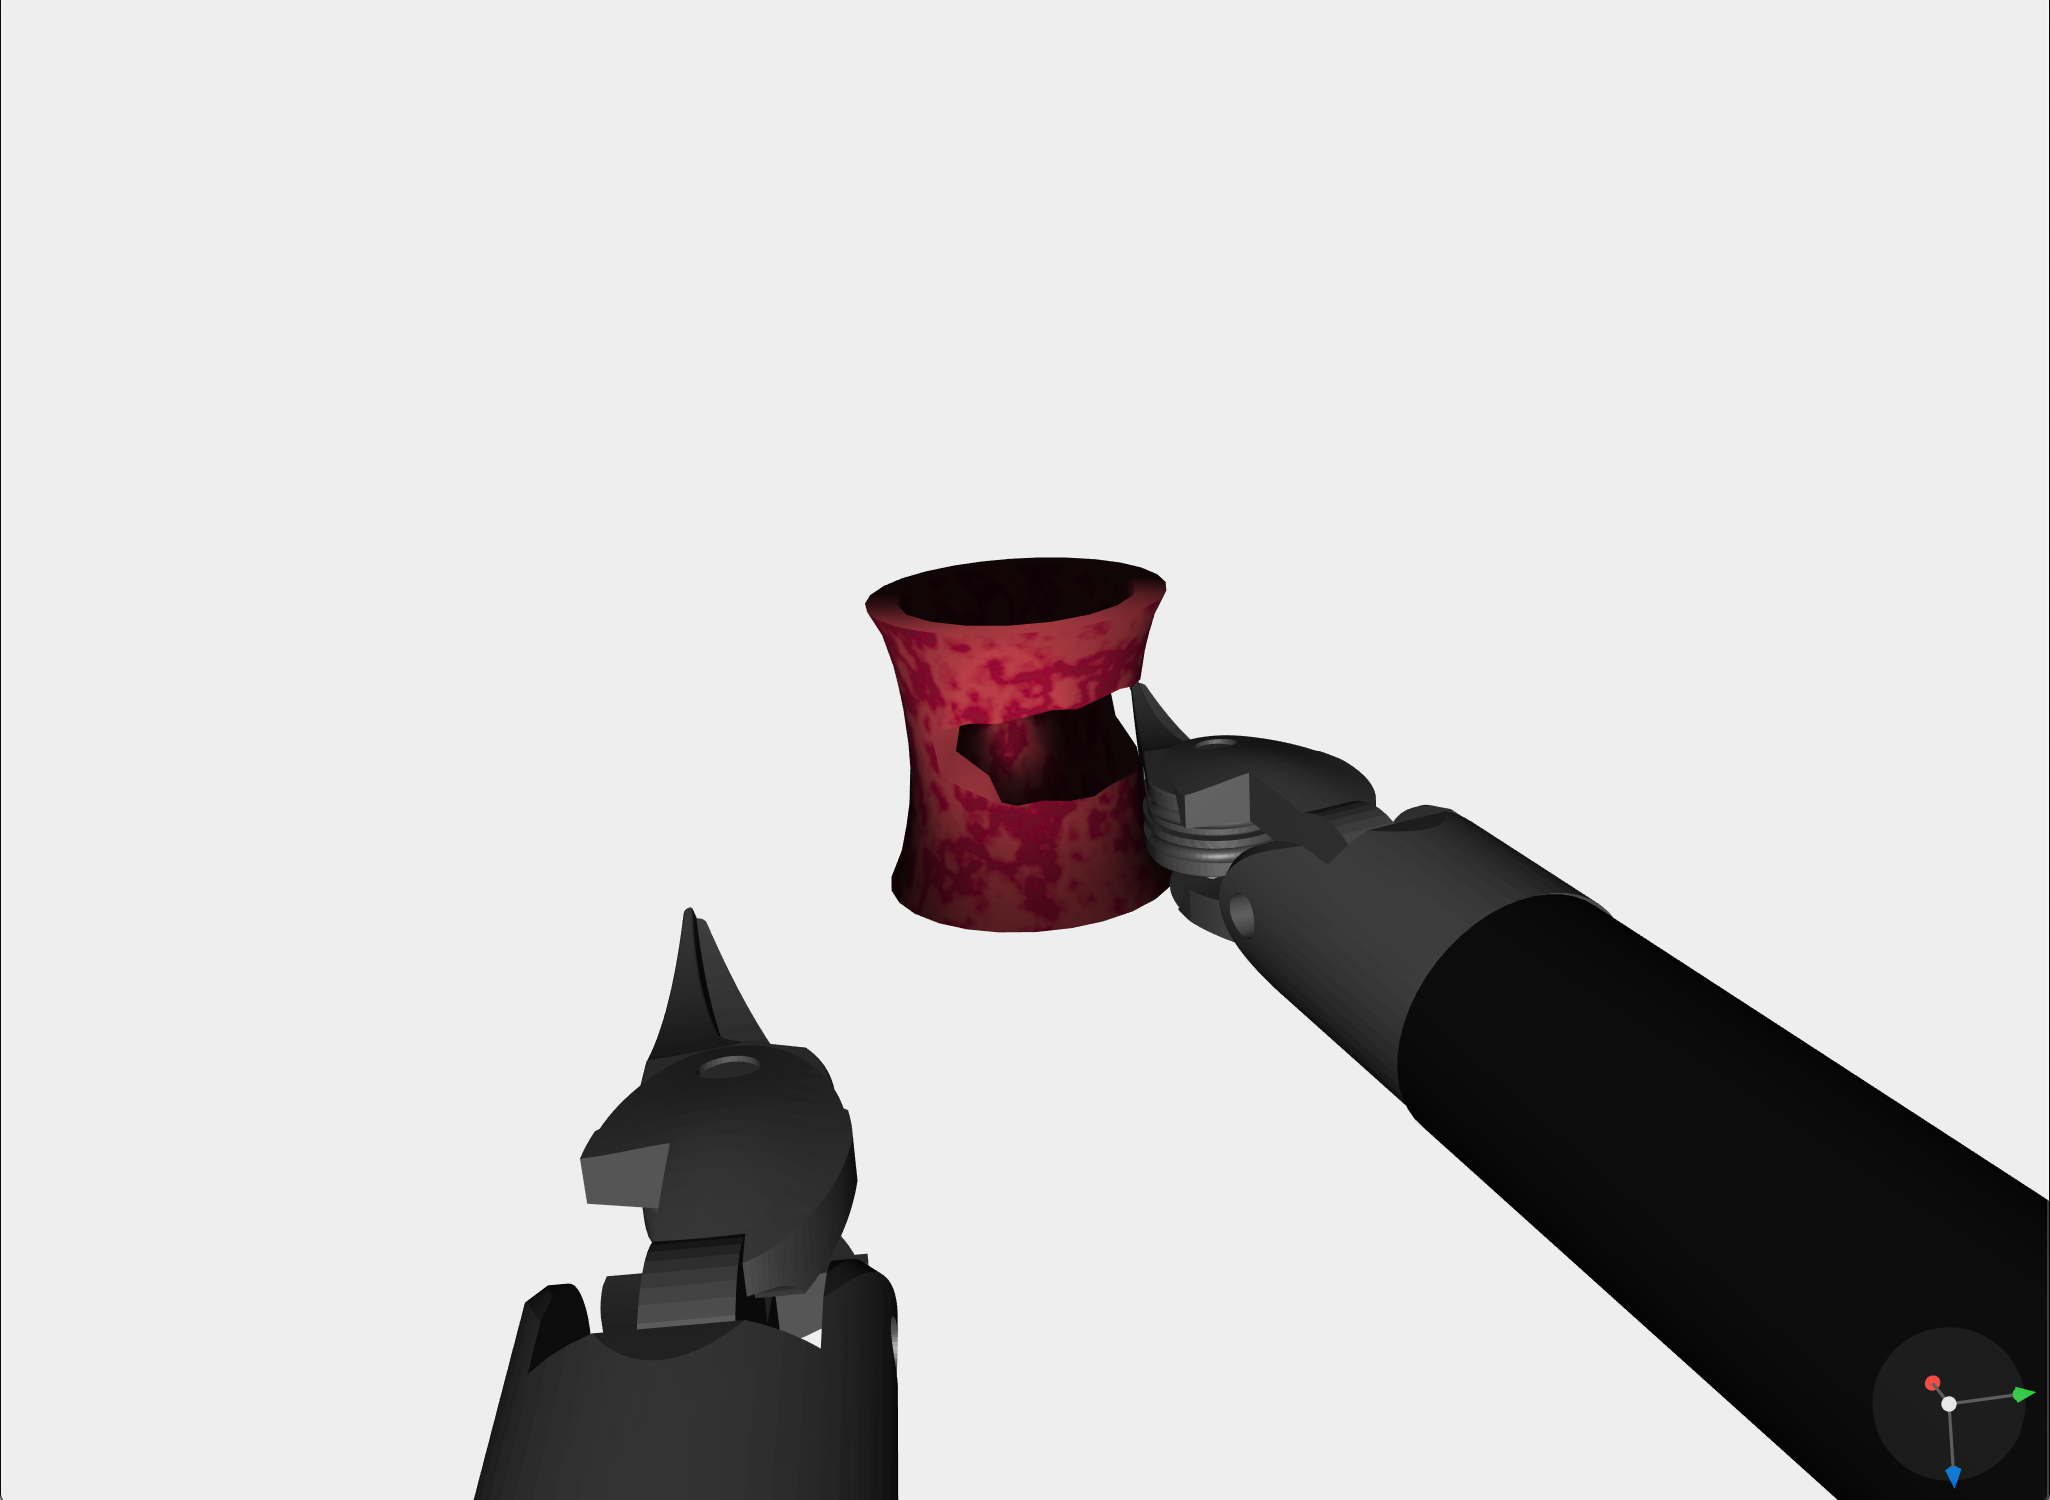
\includegraphics[width=0.49\linewidth]{integration/snap1}}\\[1.5ex]%
  \fbox{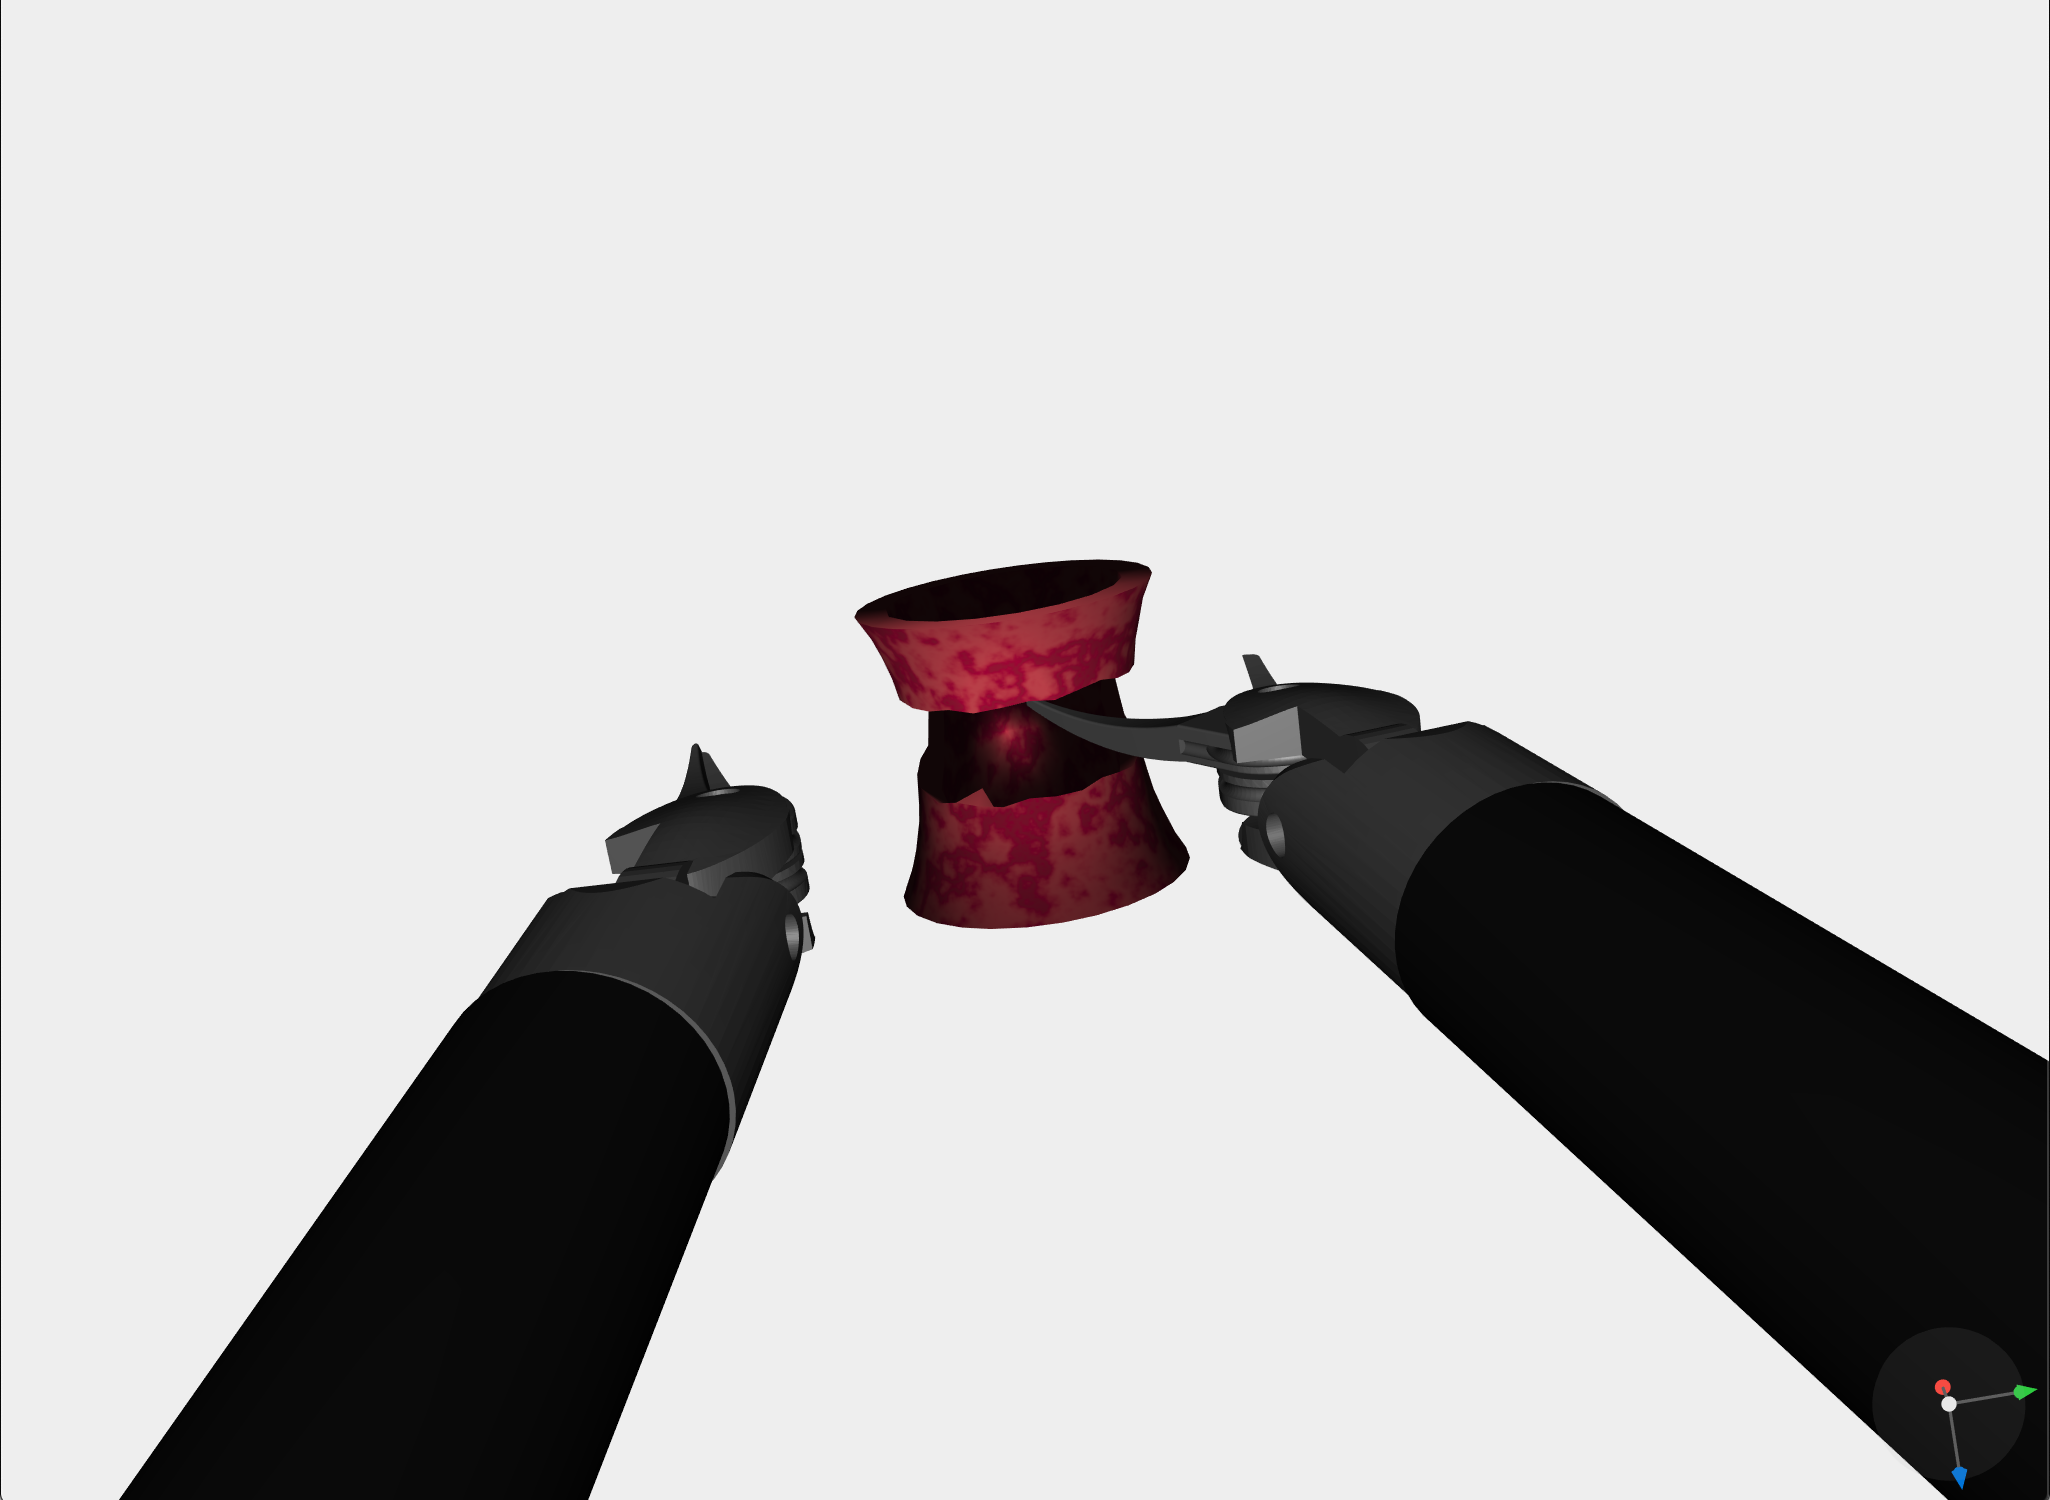
\includegraphics[width=0.49\linewidth]{integration/snap2}}\hfill%
  \fbox{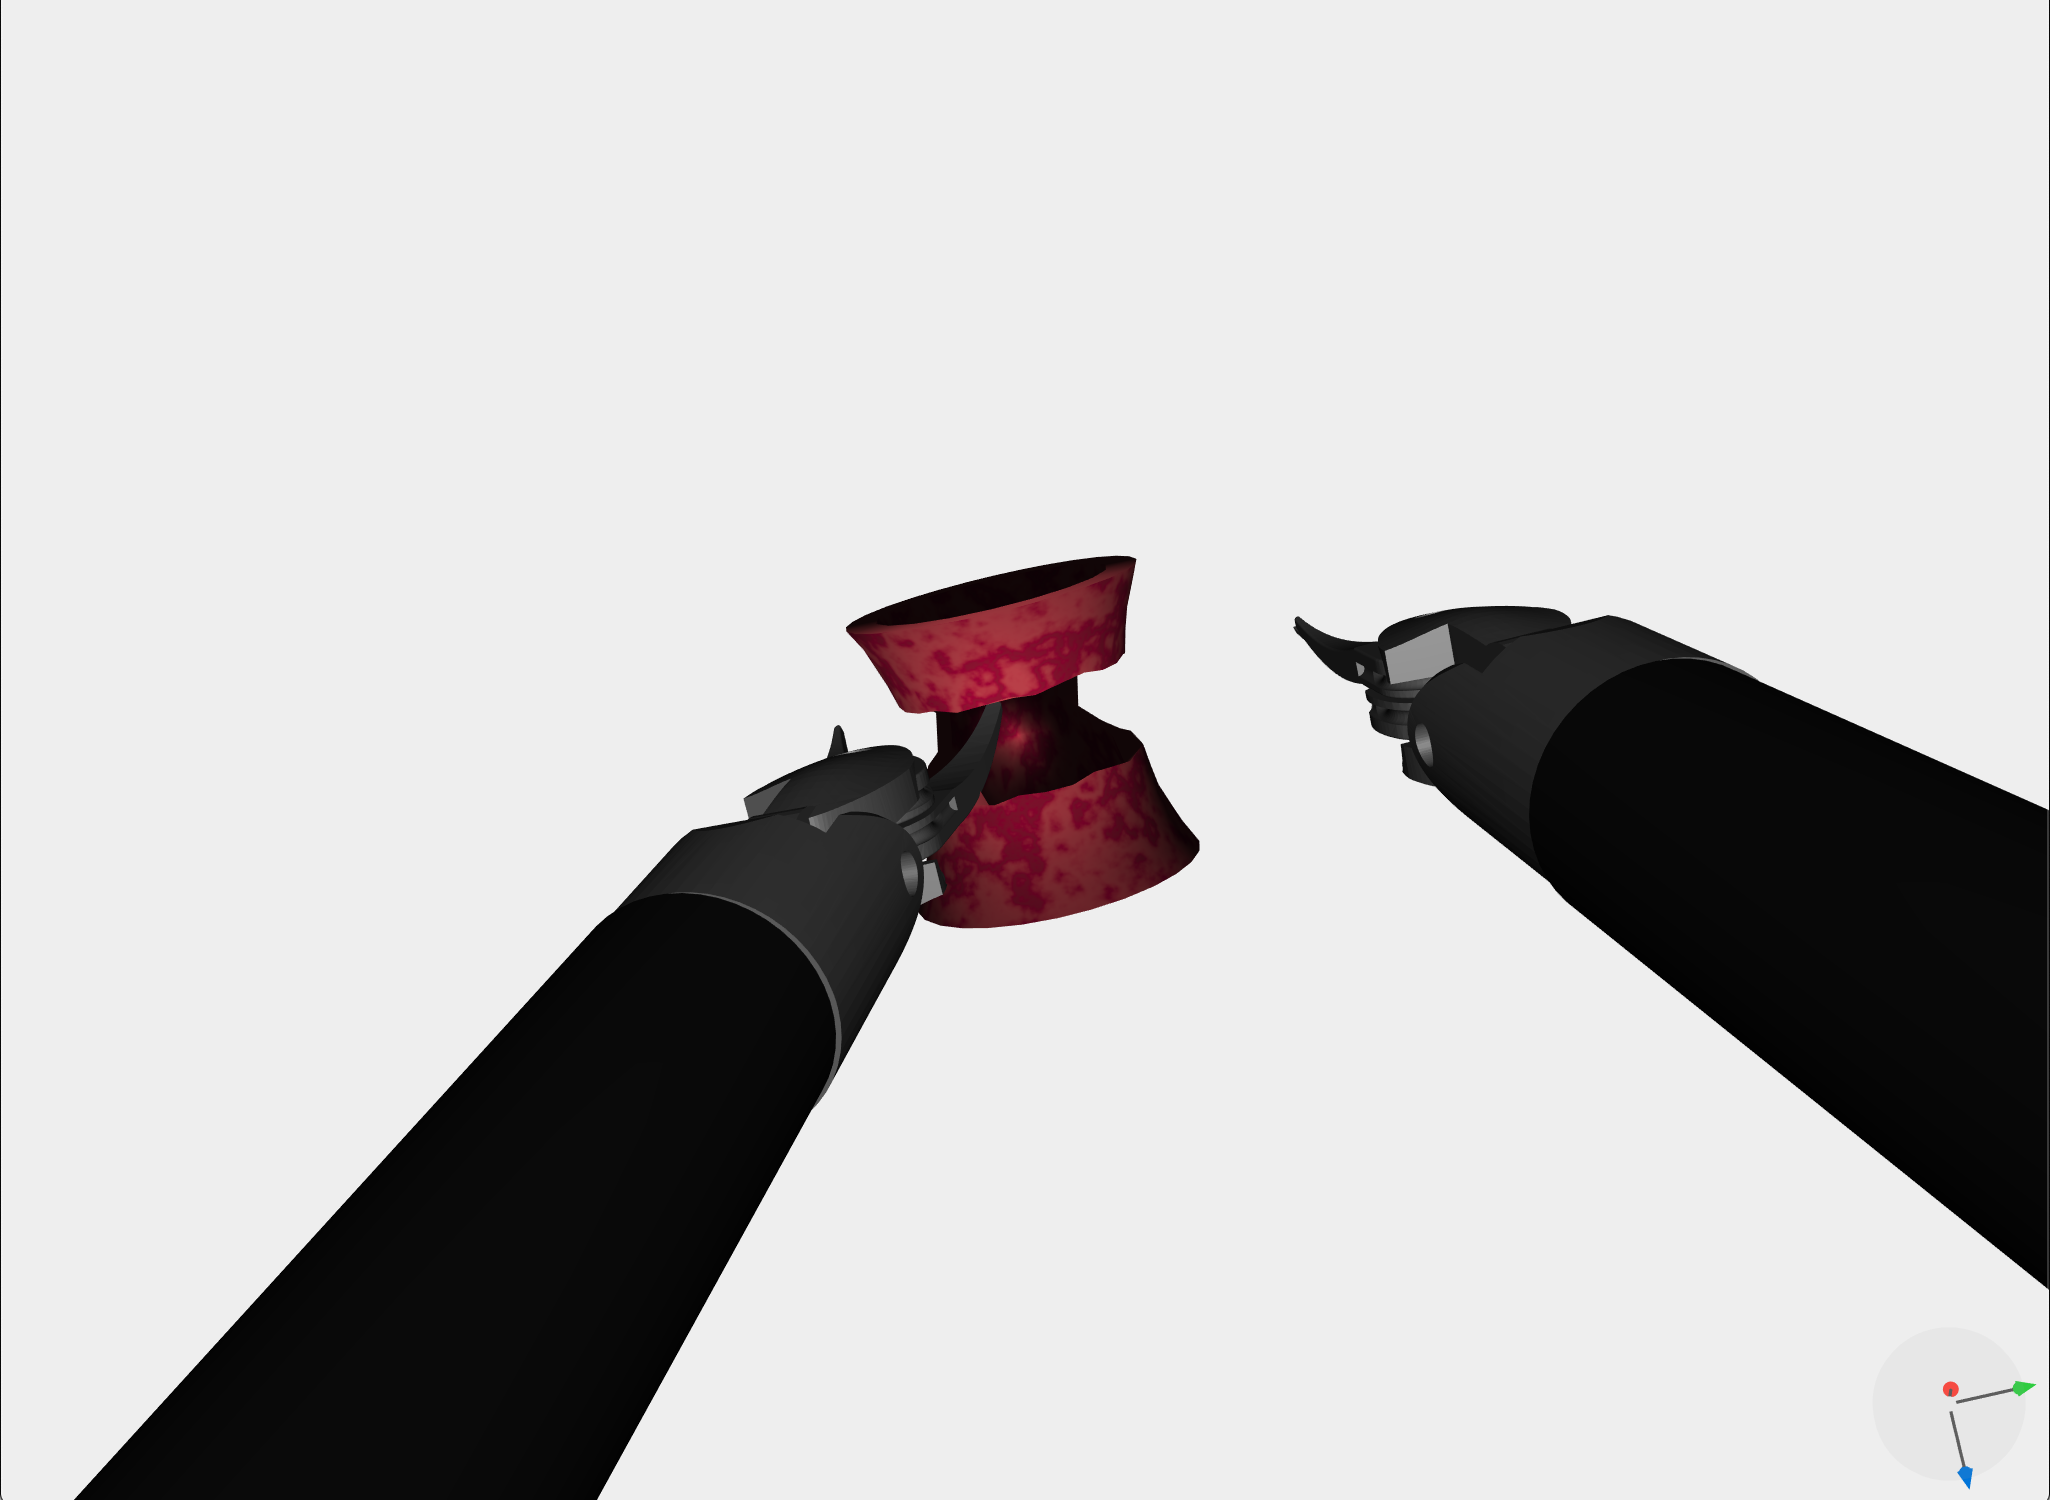
\includegraphics[width=0.49\linewidth]{integration/snap3}}\\[1.5ex]%
  \fbox{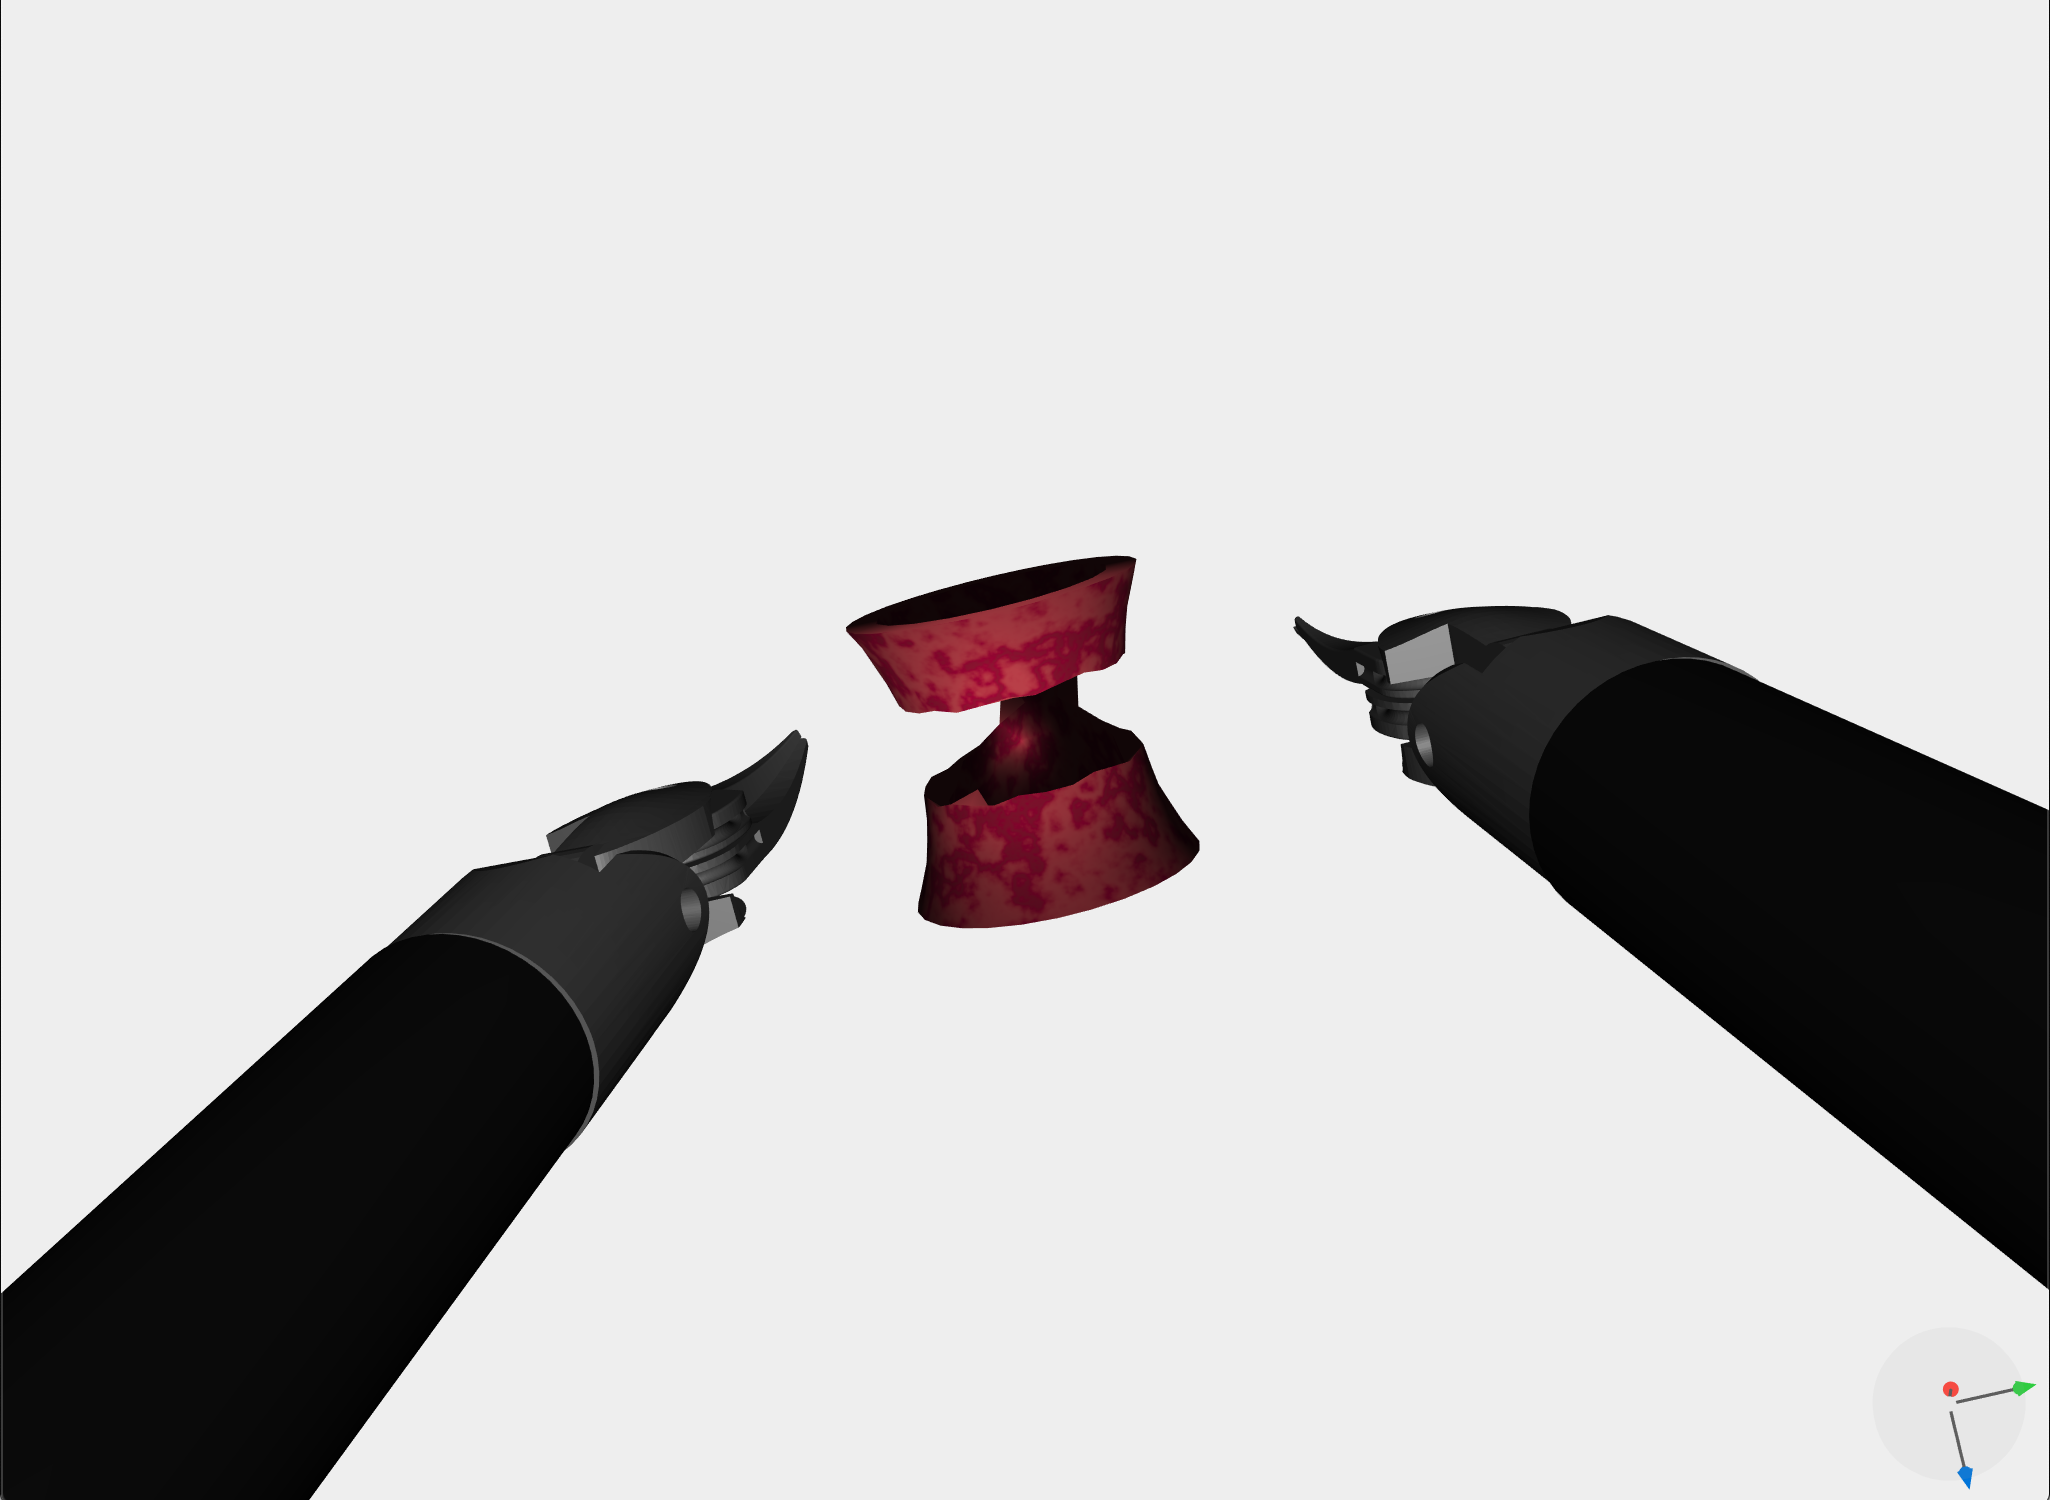
\includegraphics[width=0.49\linewidth]{integration/snap4}}\hfill%
  \fbox{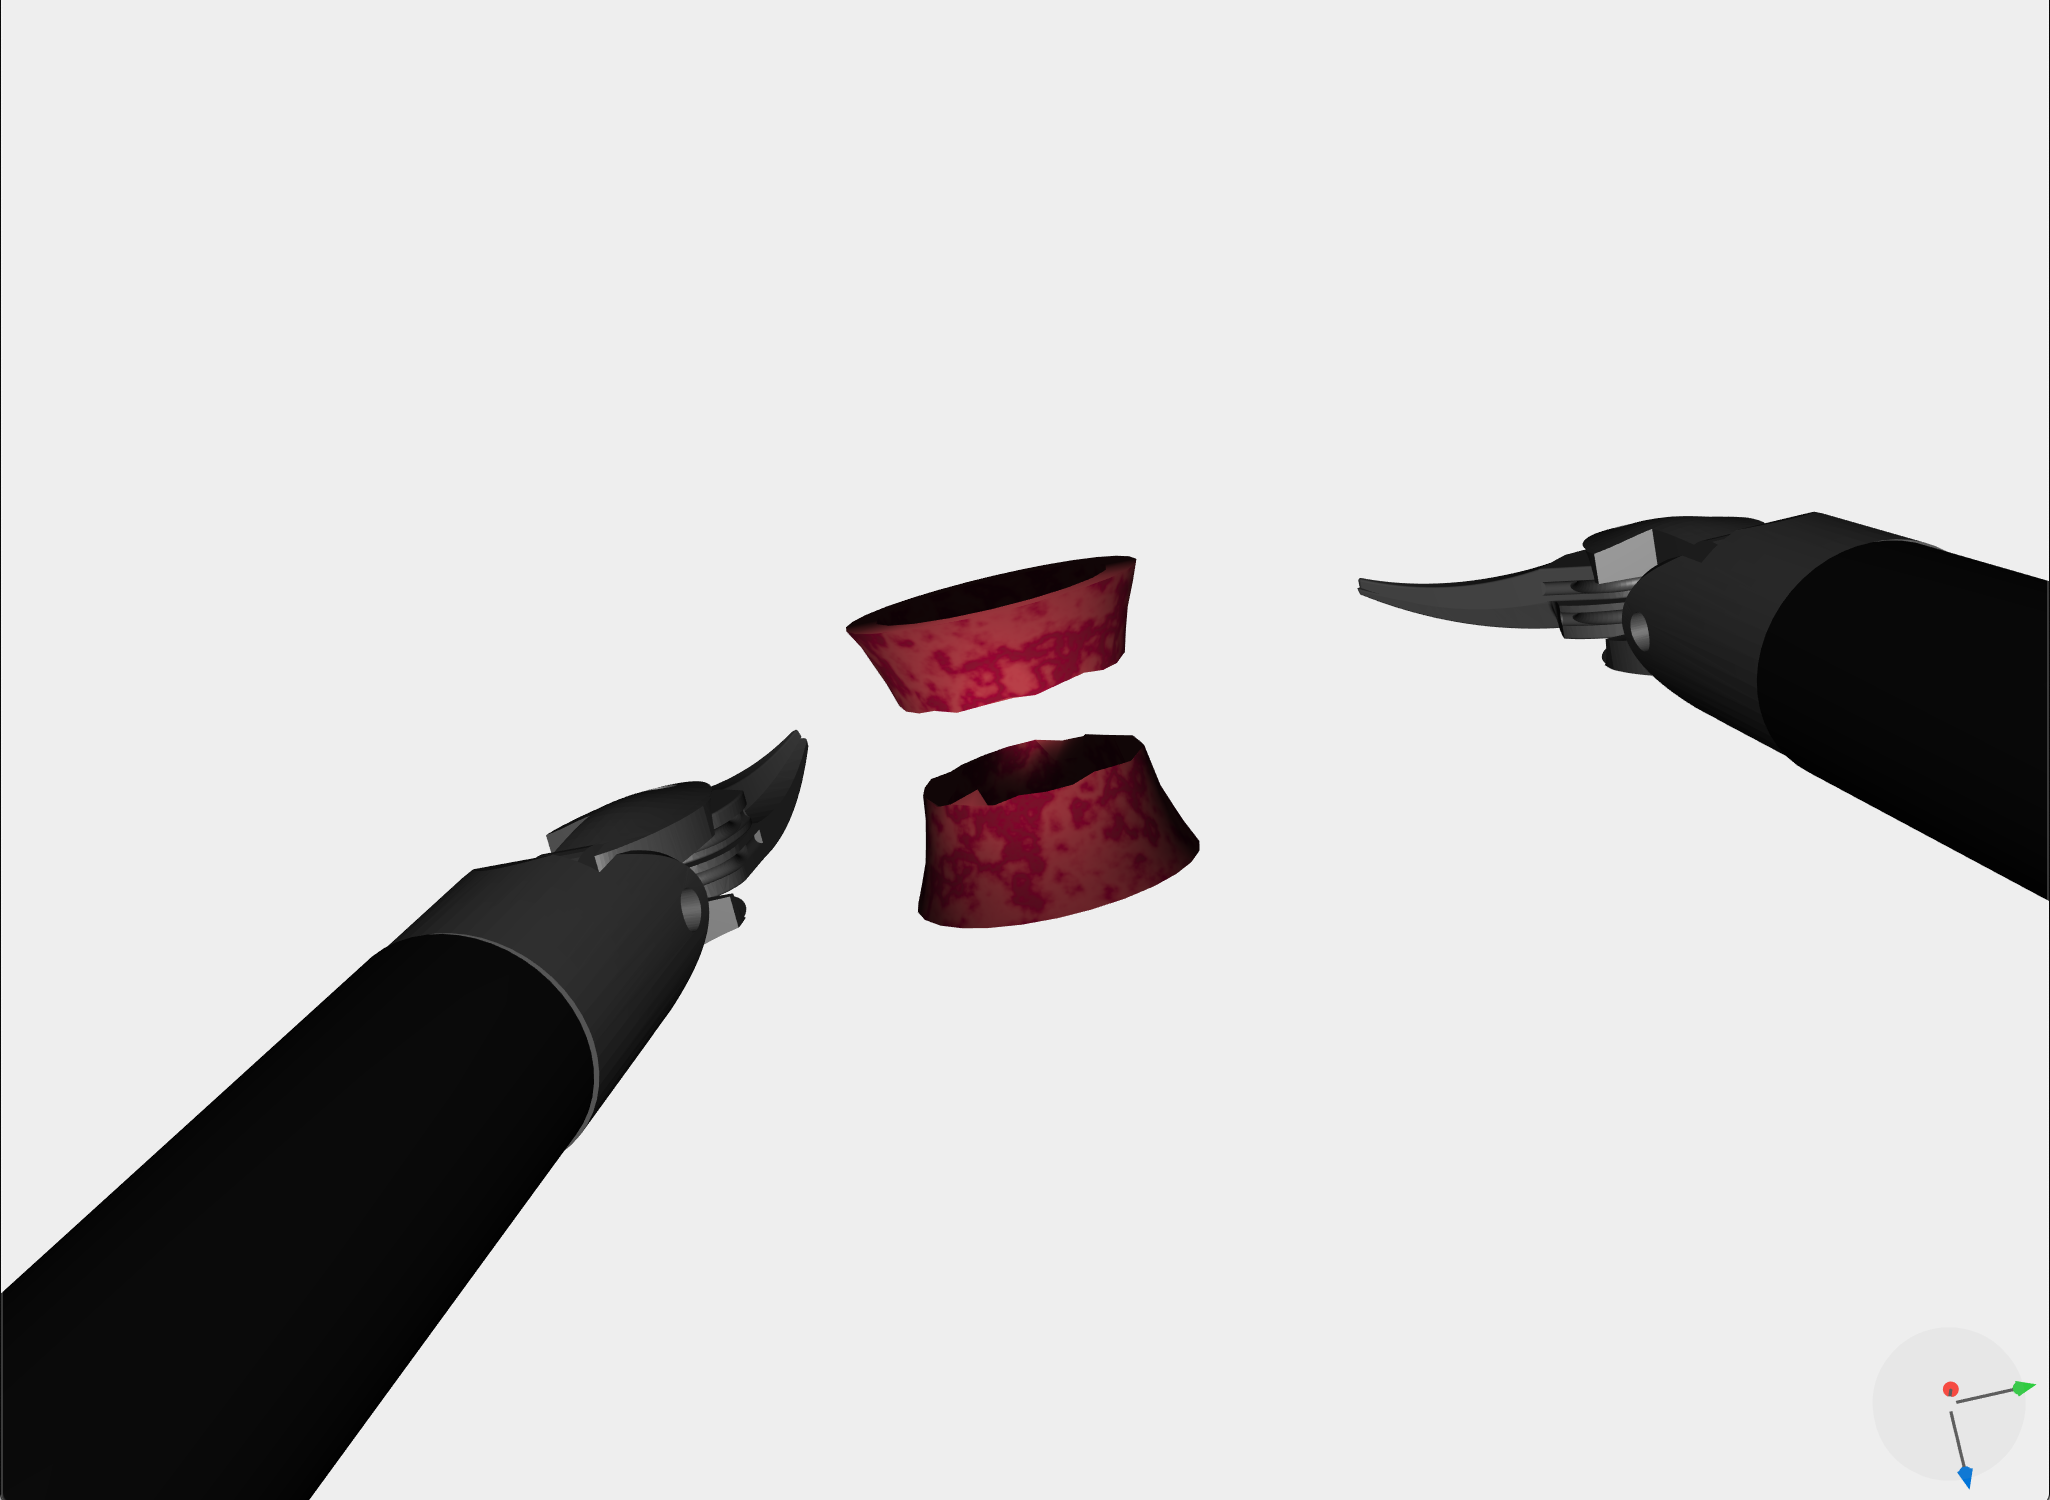
\includegraphics[width=0.49\linewidth]{integration/snap5}}\\[1.5ex]%
  \caption{---}
  \label{fig:cuts}
\end{figure}

\hrule%

\subsection{Cross-Platform Integration}
\label{sec:cross}
\subsubsection{Corrade and Magnum}
Magnum is a graphics C++ library for easy development of games, data visualization, and graphics simulation. It is a lightweight and modular platform. Magnum uses the Corrade C++ library for platform abstraction and it is its only external dependency. Magnum provides following functionalities:

\begin{enumerate}
  \item Platform abstraction via Corrade so that it can be built and run on different operating systems \eg Windows, GNU/Linux, and macOS,
  \item Minimal set of core \acr{api} for graphics development,
  \item Math library for vectors, matrix, quaternions operations to be used for graphics manipulations,
  \item Easy way to extends plugins, and
  \item Easy integration of other libraries \eg Bullet Physics SDK and DART.
\end{enumerate}

We used the following features of Magnum:
\begin{description}
  \item [Tool Simulation with Bullet Physics] One of the important aspects of medical surgery simulation is modeling tools and tool kinematics accurately. Without proper emulation of tool physics, medical simulation will not look realistic. To do so, we tried Bullet physics library with Magnum. A tool is a set of parts connected via joints. In Bullet physics simulation world, each part is represented using a rigid body (rigid body is the object in physics world). Rigid bodies are connected using constraints (joints in the real world). The benefits of using rigid bodies and constraints are when we move the object in the simulation world, we don't have to know or compute itss kinematics, it is the responsibility of the Bullet physics engine to calculate the kinematics and move the object to the correct position with correct orientation. Also Bullet physics has built-in collision shapes and collision detection algorithms which can be used for collision detection, which is another essential aspect of the medical simulation. In conclusion, Bullet physics provides a easy and faster way to develop and emulate physics involved in medical simulations without worrying about how physics work internally. \autoref{fig:tool_position_orientation} shows a tool at different positions and orientations.

  \begin{figure}
    \centering
    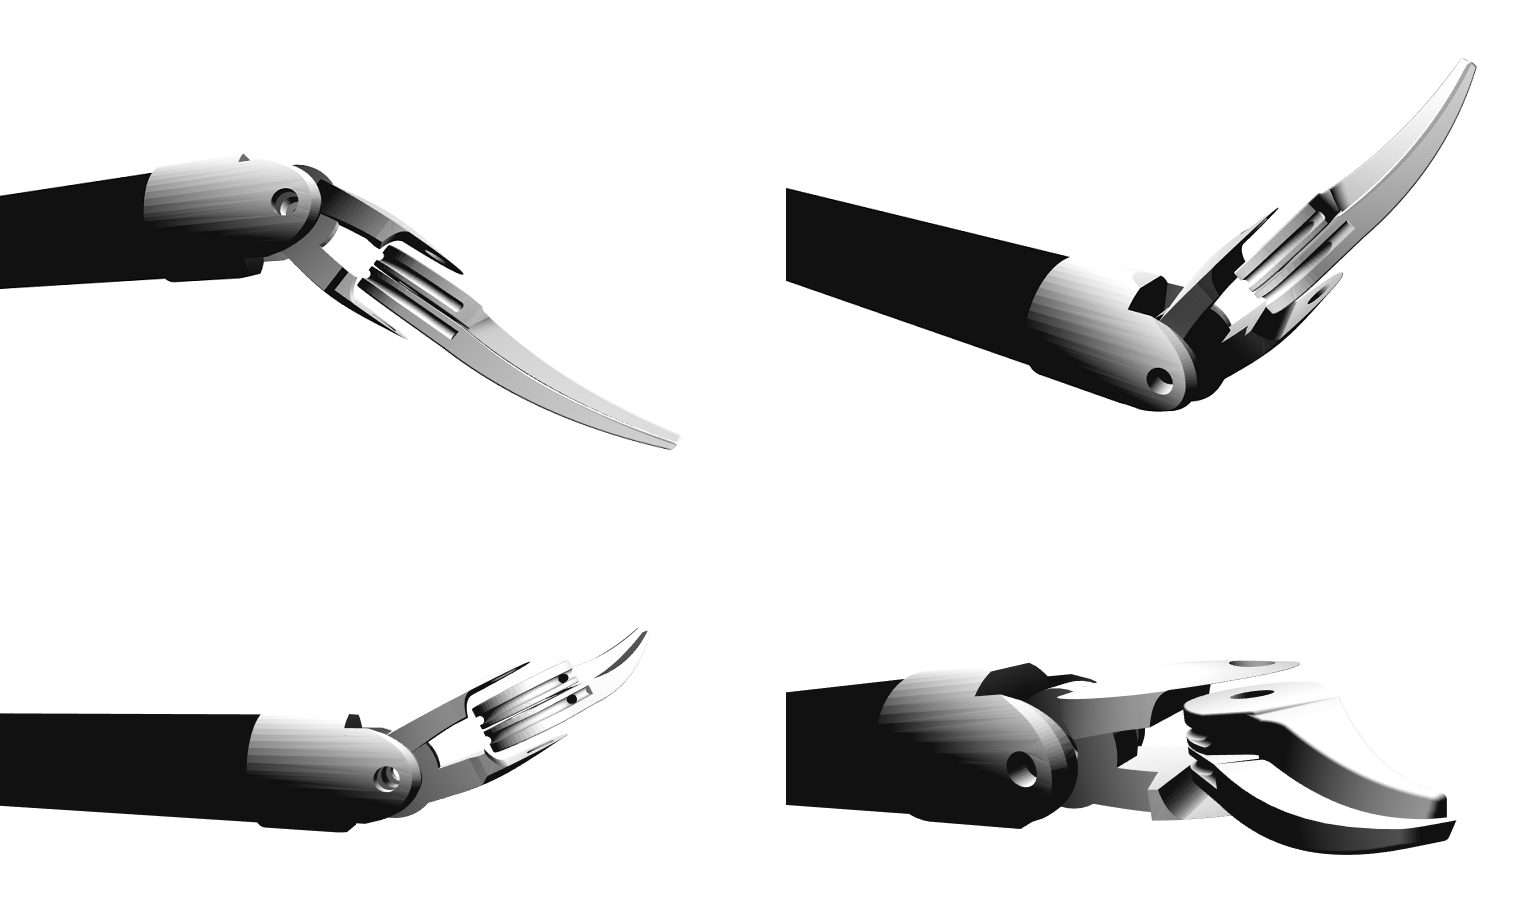
\includegraphics[width=0.8\textwidth]{integration/toolposition}
    \caption{Tool Positions and Orientations}
    \label{fig:tool_position_orientation}
  \end{figure}

  \item [Core Graphics \acr{api}] Magnum provides a core set of easy-to-use \acr{api} to develop graphical user interfaces. It abstracts OpenGL and GLSL programming which makes it convenient to use and has set of mathematical \acr{api} for doing graphics manipulation such as object translation and rotation using vectors and matrices. Magnum has a built-in camera object (both 2D and 3D) so that we don't have to develop custom camera objects. It also provide built-in meshes for basic shapes \ie spheres, cylinders, and cubes, which can be used by the user to build graphical objects.
\end{description}

\subsection{User Interface}
\label{sec:ui}
%\subsection{\st{Context-sensitive Messages}}
\subsubsection{Eye-tracking Interaction}
Eye-tracking interaction provides another dimension to interact with the system. This is useful in surgical simulation systems because both hands will be occupied while manipulating surgical tools. With a head tracker, a user can zoom, rotate, and move the camera using its head motion. With an eye tracker, a user can select menu entries, click on any button in the system using their eye motion. For this purpose we developed an eye and head tracking system using Tobii's eye/head tracking \acr{api} and integrated it with our simulator. The operating distance of the Tobii 4C eye tracker is from \SI{50}{\centi\metre} to \SI{90}{\centi\metre}. It can work with screen sizes of \SI{27}{in} with 16:9 aspect ratio or \SI{30}{in} with 21:9 aspect ratio. We implemented zoom in, zoom out, left rotation, right rotation, top movement and down movement using head position and we implemented detection of the position where user is looking in the screen using eye position. \autoref{fig:tobii_eye_tracker} shows a Tobbi 4C eye tracking device.

\begin{figure}
  \centering
  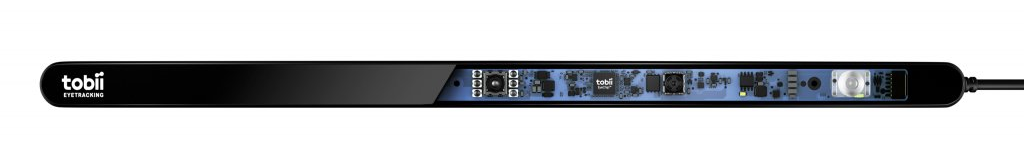
\includegraphics[width=1.0\textwidth]{integration/tobii}
  \caption{Cutaway view of the Tobii 4C eye tracker}
  \label{fig:tobii_eye_tracker}
\end{figure}

\subsubsection{Twee Integration}
To simulate the grasper in the da Vinci Xi console, we have integrated an accessory for the Geomagic Touch device known as \enquote{Twee.} This accessory replaces the removable pen with an additional degree of freedom. The device has one button and a grasper which allows us to detect the opening and closing of two fingers. In each iteration, it outputs the status of the button and the angle of the opening. The angle goes from \SI{0}{\degree} when closed up to approximately \SI{30}{\degree} when fully opened.

One of the functionality that has been implemented by us helps to dynamically detect whether the user is using the accessory with the haptic device or if they are just using the stylus.

To simulate a real scissor, we have implemented a feature to trigger cutting based on the angle of scissors. Based on an arbitrary threshold, when the user closes the scissors and crosses the minimum threshold, the snip is triggered. Once a snip has been triggered, to prevent the cutting operation from continuously being triggered, we use a boolean to disable snipping until the user has opened the scissors to go above the minimum threshold angle.

We have three states for the scissors based on the angle of the scissor, initial state is when cutting is inactive and the scissor is fully opened. Second state is when the scissors are partially closed which triggers progressive cutting. When the scissors are almost fully closed, the single snip function is triggered.

\begin{figure}
  \centering
  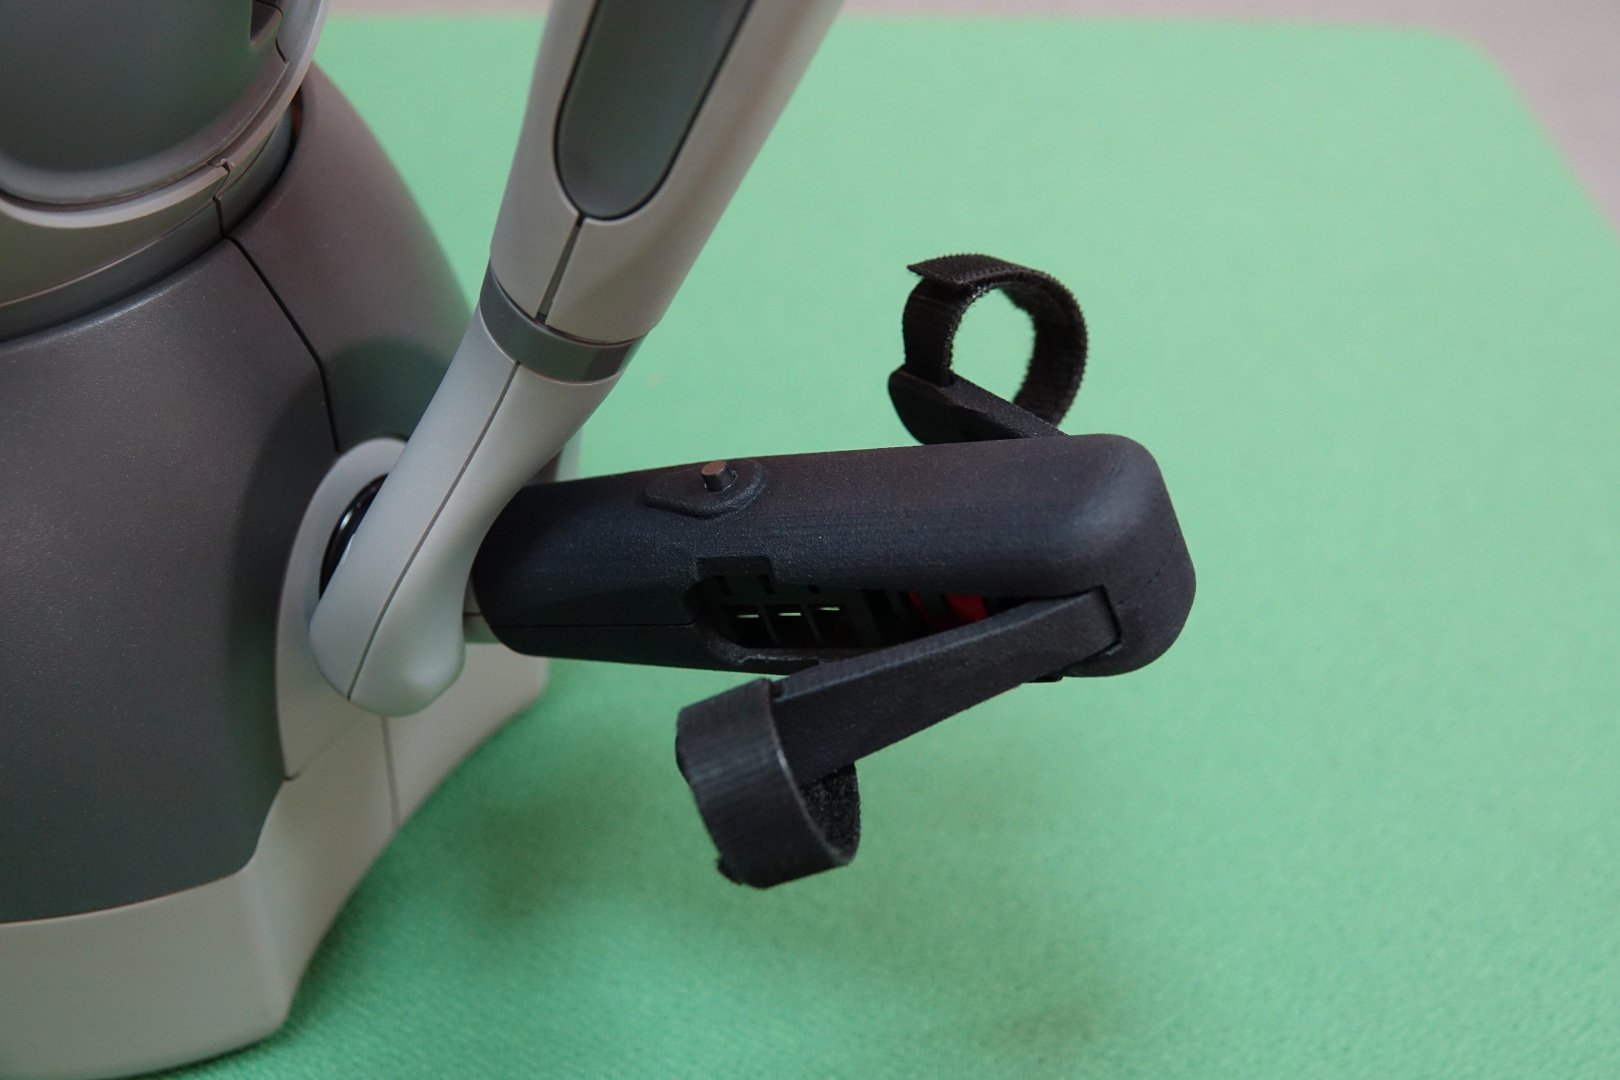
\includegraphics[width=1.0\textwidth,frame]{integration/twee}
  \caption{Twee connected to a 3D Touch device}
  \label{fig:twee}
\end{figure}

\subsubsection{Basic Console}
\autoref{fig:3d_console} presents an isometric view of a basic wooden console that contains the interfaces for manipulation and visualization. A surgeon can sit in front of the structure, rest his arms on the frontal support and access with his hands both styluses of the haptic devices while observing a surgical field through the \acr{vrh}.

\begin{figure}
  \centering%
  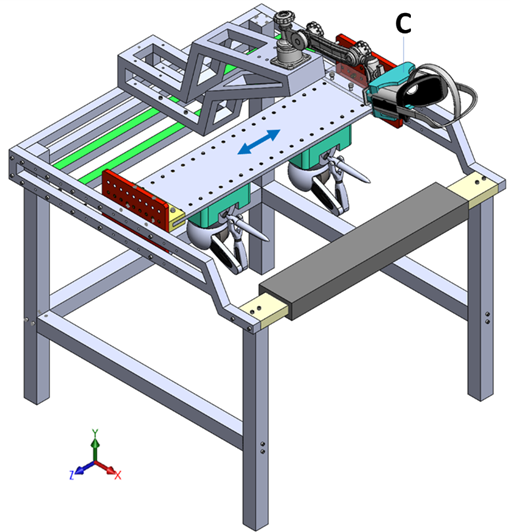
\includegraphics[width=0.55\textwidth]{integration/console_iso}
  \caption{Isometric view of the basic console}
  \label{fig:3d_console}
\end{figure}

\autoref{fig:side_console} illustrates how the position of the \acr{vrh} is adjusted thanks to an articulated arm that can be rotated/tilted through the handles 1, 2 and 3 that locks its joints. Additionally, the spherical joints 4, 5 attached to a \acr{3d} printed case \enquote{C} allow fine adjustment of the device's orientation in the space.

The base is mounted atop the central part of the structure where it is secured firmly. The base of the arm can be unattached and re-positioned in the direction U.

\begin{figure}
  \centering
  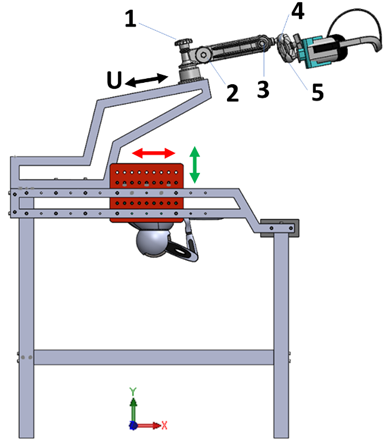
\includegraphics[width=0.55\textwidth]{integration/console_side}
  \caption{Side view of the basic console}
  \label{fig:side_console}
\end{figure}

The position of the haptic devices can be modified in three dimensions $(x, y, z)$ within the workspace of the surgeon arms. \autoref{fig:side_console} shows how these devices can be moved up/down or forward/backward by screwing its support, (board in red color), to different holes in the structure. The left/right adjustment is visible in \autoref{fig:3d_console}.

\subsubsection{Tool Collision with Soft Tissue}
Instead of using line segments as tool contact shapes, we opted to go for a cloud of points to represent the collision shape. This allows for designing collision shapes for tools with complex shapes such as blades that are curved, spiral, or crooked.

To extract the points, we developed a utility function written in Python that extracts desired points from the tool mesh using the open source application Blender. We can visually cherry pick the desired vertices in Blender, and output them using the Python script we developed to extract the set of points. Once the collision points are extracted, they are loaded into the simulator and the global position of each point with respect to the tool frame is passed through motion commits to the soft body system.

Our initial tests on deforming the urethra with the points resulted in over constraining due to a higher density of points. To reduce the density while covering most of the blade surface, we generated points that spiral around the blade.

\begin{figure}
  \centering
  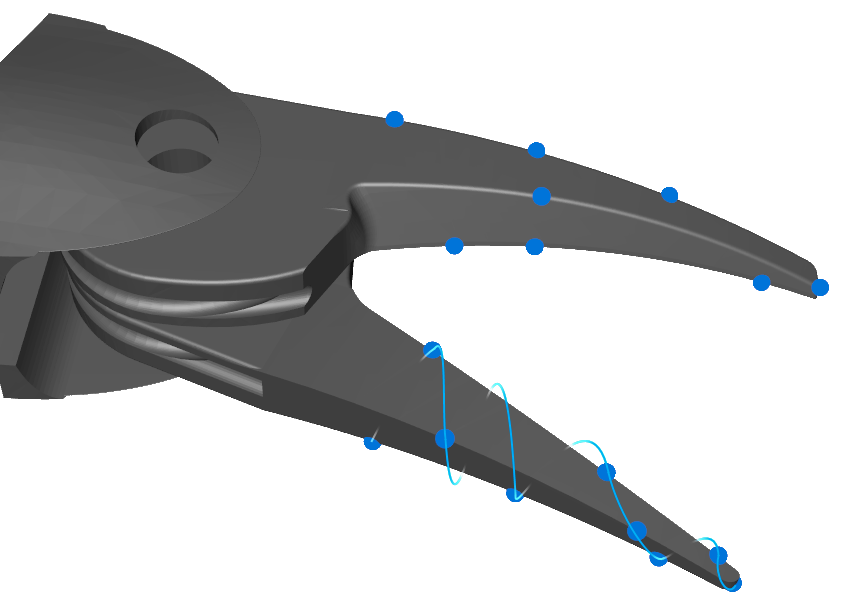
\includegraphics[width=0.45\textwidth]{integration/toolspiral}
  \caption{Tool points on the blade following a spiral path}
  \label{fig:spiral_tool}
\end{figure}

%\section{Haptic Control}
\label{sec:haptic}
%\subsection{\st{Color-coded Tools}}
%\subsection{\st{Basic Force Feedback}}

\subsubsection{Stereoscopic Rendering}
\label{sec:stereo}
%\subsection{\st{Endoscopic Camera Control}}
\acr{vr} is a simulated experience that can be similar to or completely different from the real world. A person using virtual reality equipment is able to look around the artificial world, move around in it, and interact with virtual features or items.

Using this technology we have rendered the scene in the virtual environment and the user can see it in the \acr{3d} world using the \acr{vr} headset. We have used Oculus Rift (\autoref{fig:oculus_rift}), Oculus Rift S (\autoref{fig:oculus_rift_s}), and Oculus Quest over Oculus Link (\autoref{fig:oculus_quest}), to test and visualize the scene.

\begin{figure}
  \centering
  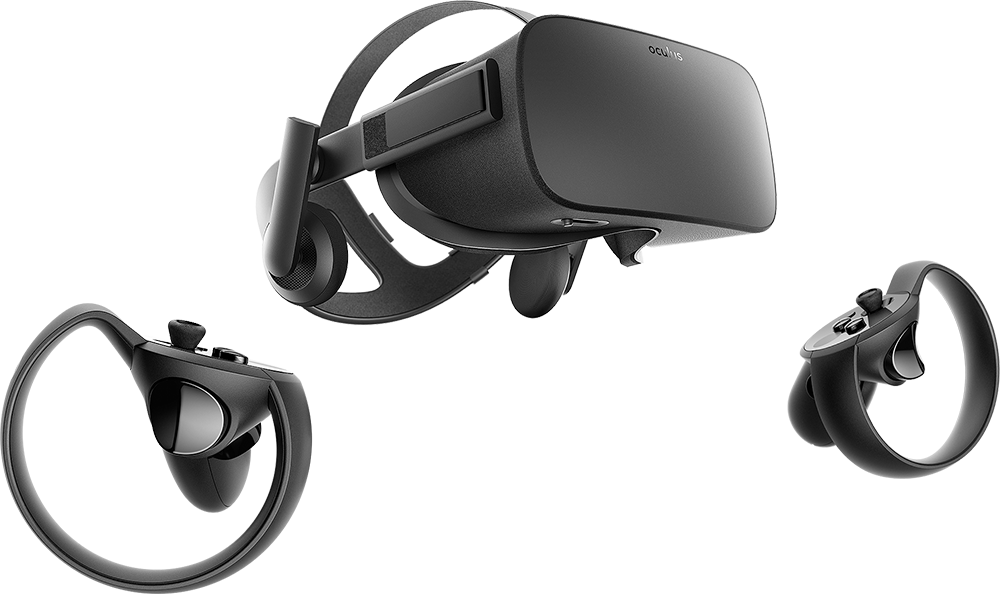
\includegraphics[width=0.75\textwidth]{integration/oculus-rift}
  \caption{Oculus Rift}
  \label{fig:oculus_rift}
\end{figure}

\begin{figure}
  \centering
  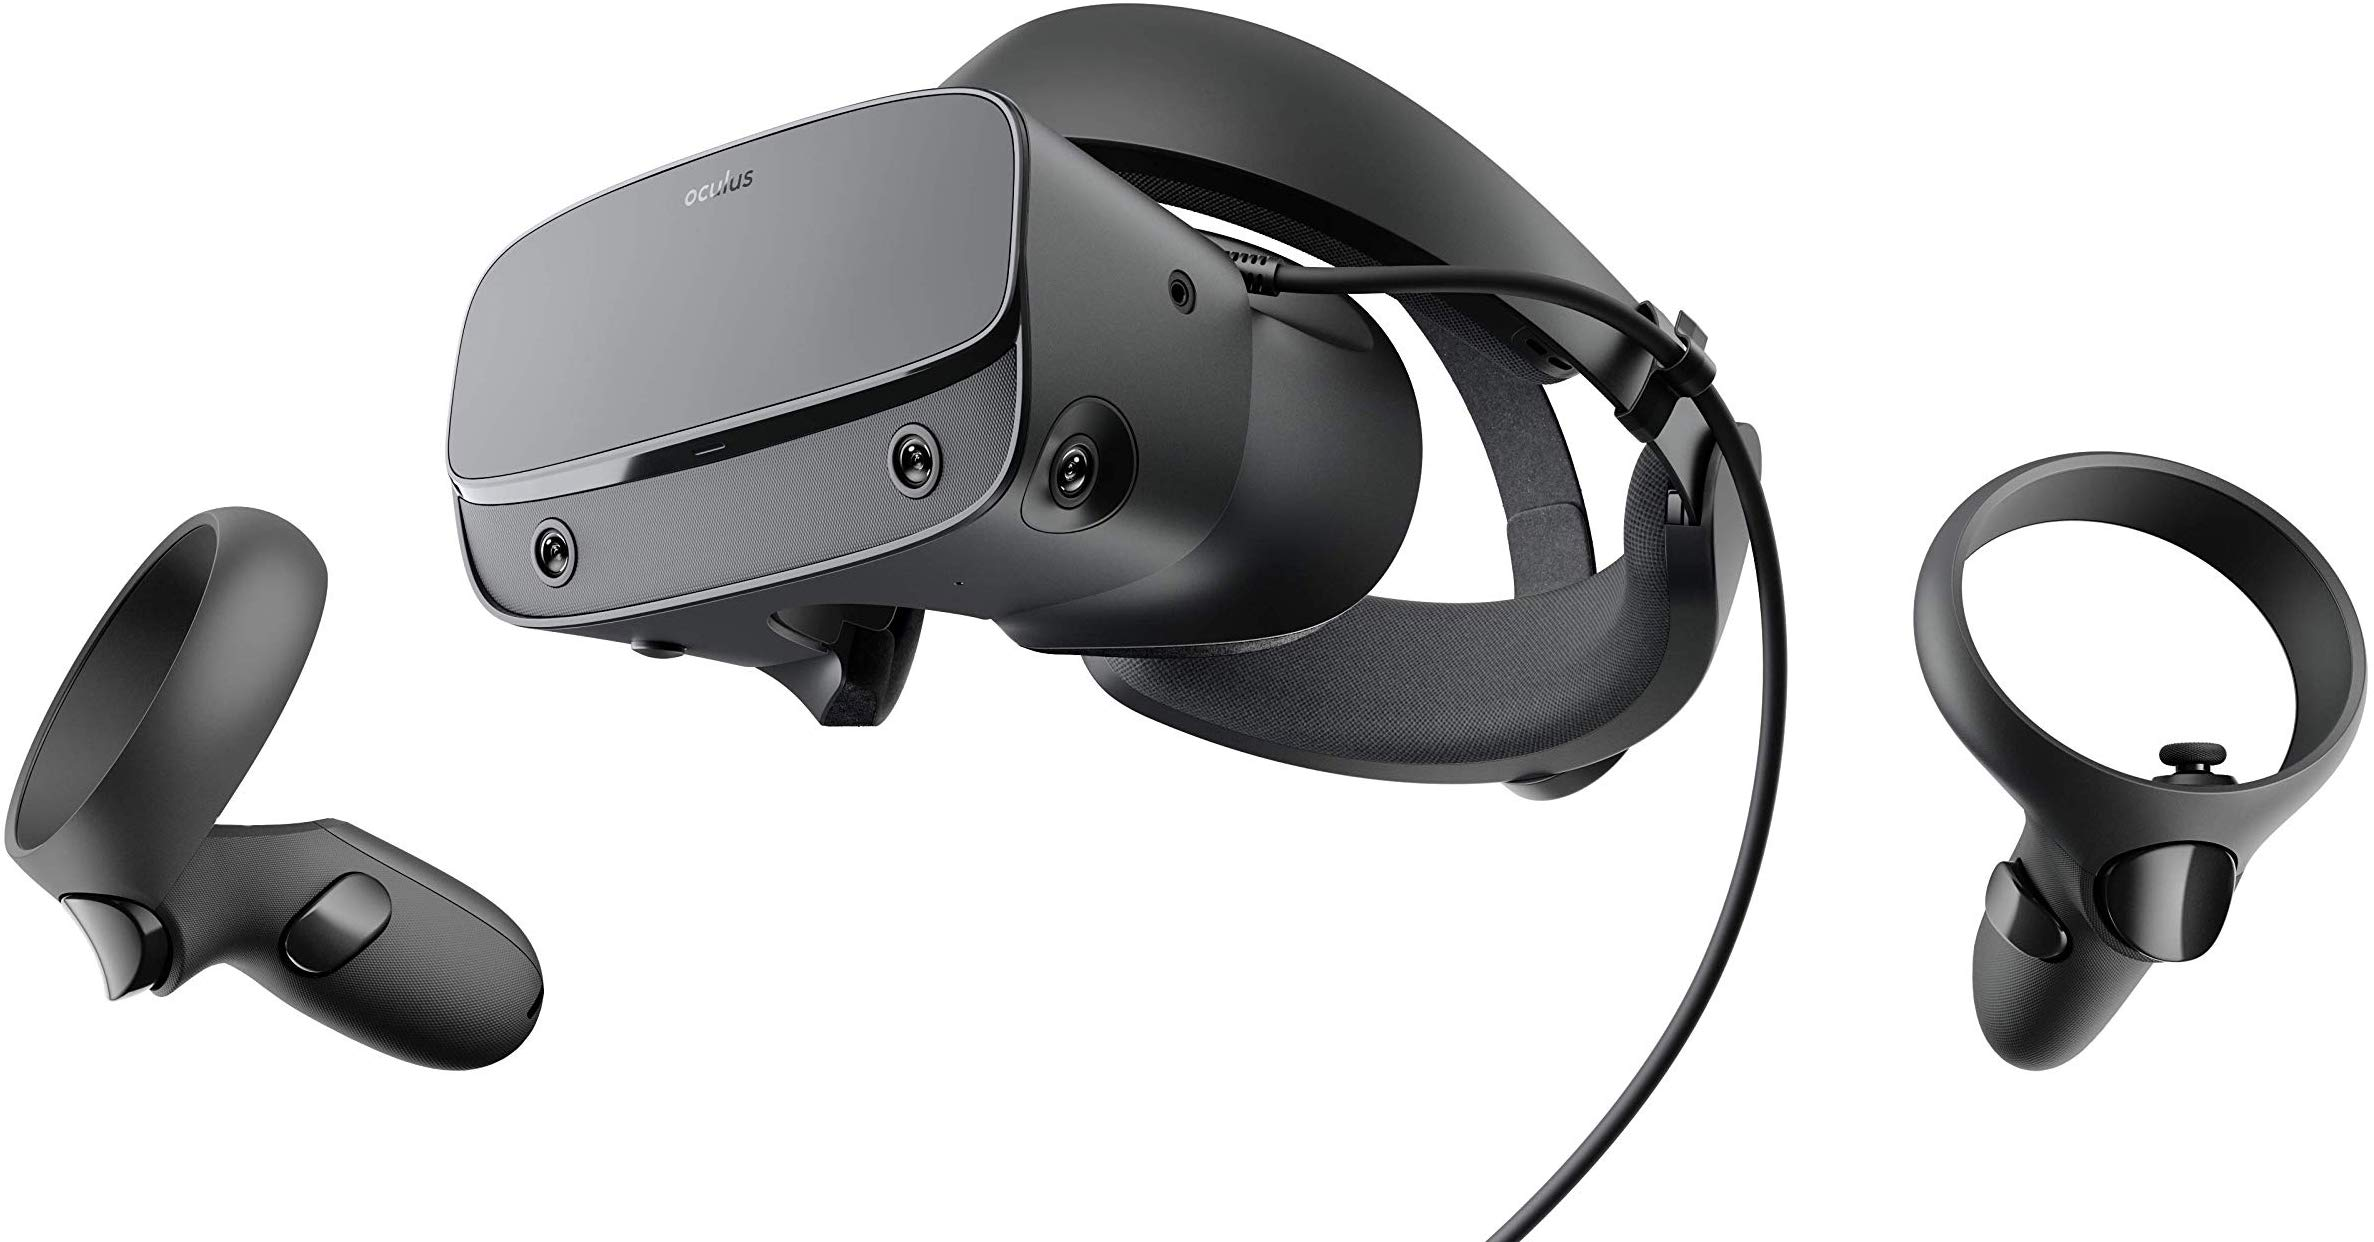
\includegraphics[width=0.75\textwidth]{integration/oculus_rift_s}
  \caption{Oculus Rift S}
  \label{fig:oculus_rift_s}
\end{figure}

\begin{figure}
  \centering
  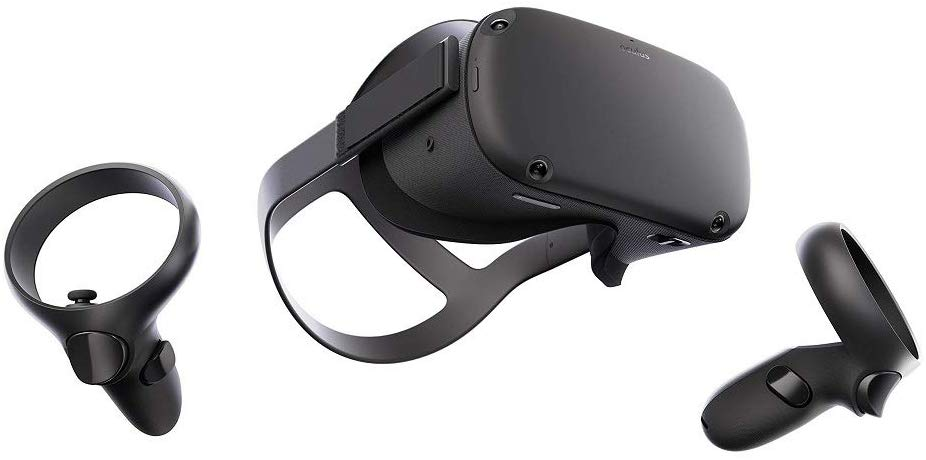
\includegraphics[width=0.75\textwidth]{integration/oculus_quest}
  \caption{Oculus Quest}
  \label{fig:oculus_quest}
\end{figure}

\begin{enumerate}
  \item Development environment specification:
  \begin{itemize}
    \item Visual Studio 2019 with C++17 (\url{https://visualstudio.microsoft.com/downloads/})
    \item OpenVR SDK (\url{https://github.com/ValveSoftware/openvr})
    \item Steam VR (\url{https://www.steamvr.com/en/})
    \item CMake (\url{https://cmake.org/download/})
  \end{itemize}
  The installation and setup of these tools is available at the respective links.

  \item High-Level Architecture:
  OpenVR, an open source programming interface created by Valve to allow communication with a \acr{vr} system.  OpenVR serves in this regard, and is compatible with all major \acr{hmd}'s. SteamVR, Valve's commercial implementation of OpenVR, serves additionally as the main software driver for the Oculus \acr{hmd}'s. Our simulator software submits the scene to OpenVR for both eyes, and OpenVR passes the data to the SteamVR driver and finally to the \acr{vr} headset.

  \begin{center}
  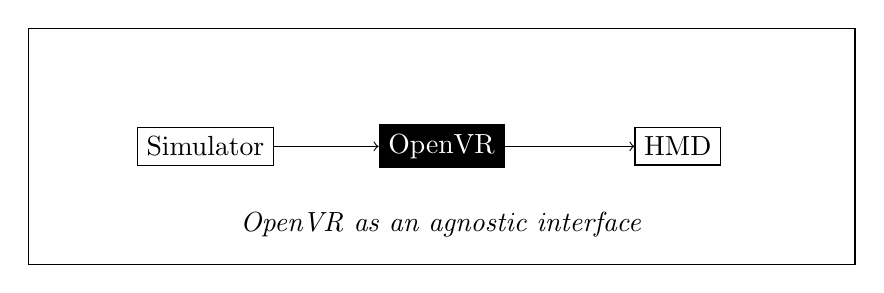
\begin{tikzpicture}
    \centering
    \node[draw, minimum height=3cm, minimum width=10.5cm] (Archi) at (5,0) {};
    \node[draw] (Simulator) at (2,0) {Simulator};
    \node[draw,fill=black,text=white] (OpenVR) at (5,0) {OpenVR};
    \draw[->] (Simulator) to (OpenVR);
    \node[draw] (Oculus) at (8,0) {HMD};
    \draw[->] (OpenVR) to (Oculus);
    \node at (5, -1.0) {\emph{OpenVR as an agnostic interface}};
  \end{tikzpicture}
  \end{center}

  \item Render Scene:
  The scene is rendered for both eyes with respect to the \acr{vr}'s Model-View projection. When the scene is rendered to the \acr{vr} headset, the scene will be placed in the world position when the user can move around the scene to visualize it in the virtual world (\autoref{fig:vr_scene}).

  \begin{figure}
    \centering
    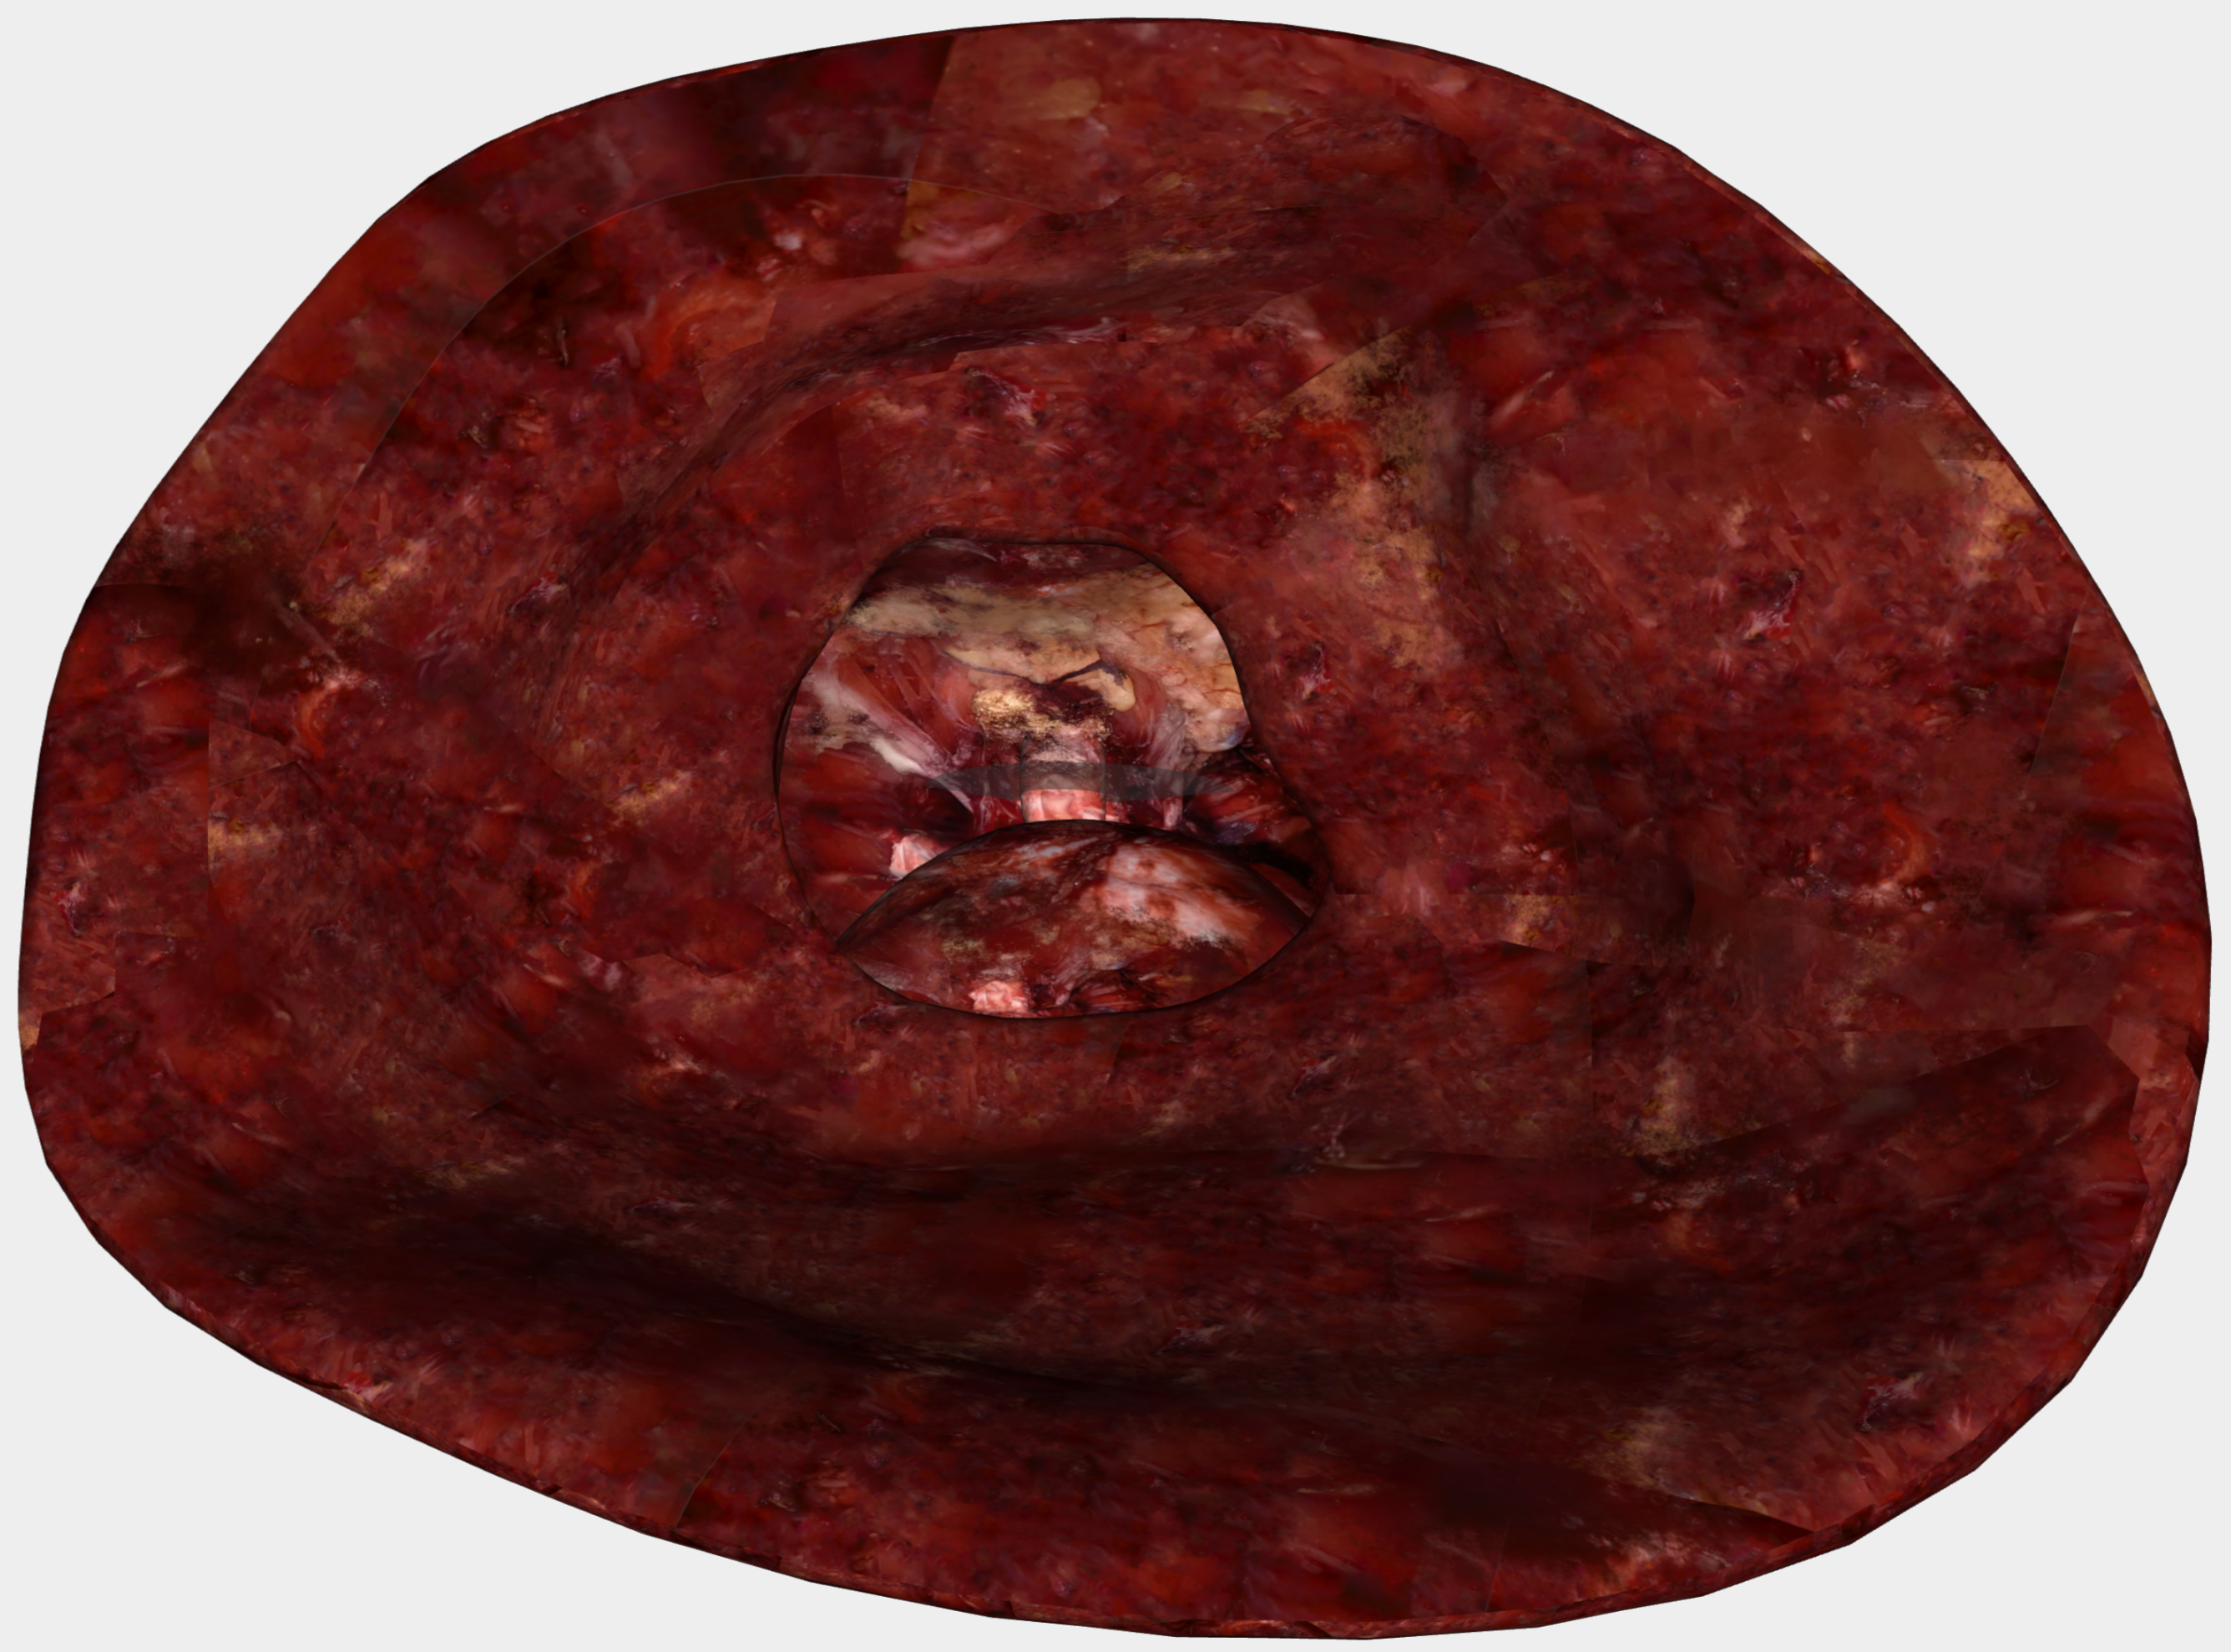
\includegraphics[width=0.8\textwidth,frame]{integration/VR_Scene}
    \caption{Scene rendered in \acr{vr}}
    \label{fig:vr_scene}
  \end{figure}

  \item Controller:
  \acr{vr} controllers offer the buttons and joysticks of a traditional gamepad with added motion tracking and a layout designed to be used without sight of the hands. The controllers are used to move the surgical tools. With the location and orientation of the controller, the movement of the surgical tools is defined. Using the controller, the user can translate, rotate and reset the position of the scene (\autoref{fig:touch_controllers}). The \textsf{X} and \textsf{Y} buttons on the controller give the ability to navigate between two modes: one where the scene is fixed to the headset and another where the scene is in world coordinates and the user and move around the scene to visualize it.

  \begin{figure}
    \centering
    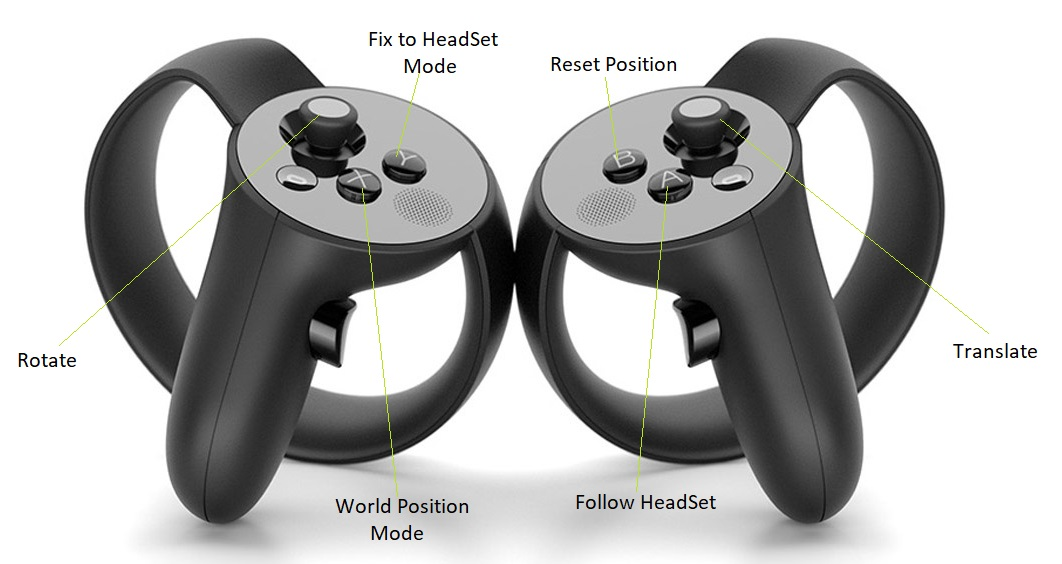
\includegraphics[width=1.0\textwidth]{integration/controllers}
    \caption{Controllers button-to-action mapping}
    \label{fig:touch_controllers}
  \end{figure}
\end{enumerate}

\paragraph{Holographic Rendering with the Looking Glass}
Looking Glass is a holographic display that generates 45 distinct views of a 3D scene to give an illusion of depth without requiring the user to wear any glasses, or headset. The lenticular lens of the looking glass distributes these 45 unique views to the user allowing for more than one user and to view from more angles.
Looking Glass outputs a horizontal-parallax-only light field image made of 45 distinct views. Each light field is stored in their own format known as \enquote{quilt.} To display any 3D environment in the Looking Glass, we have to construct a quilt which consists of the 45 views represented in a grid format. Each of the views is rendered to a texture, which is then copied on to the quilt using a copy function provided by their \acr{api}. Once the quilt is properly constructed, another \acr{api} function is used for rendering the light field using the quilt.

\begin{figure}
  \centering
  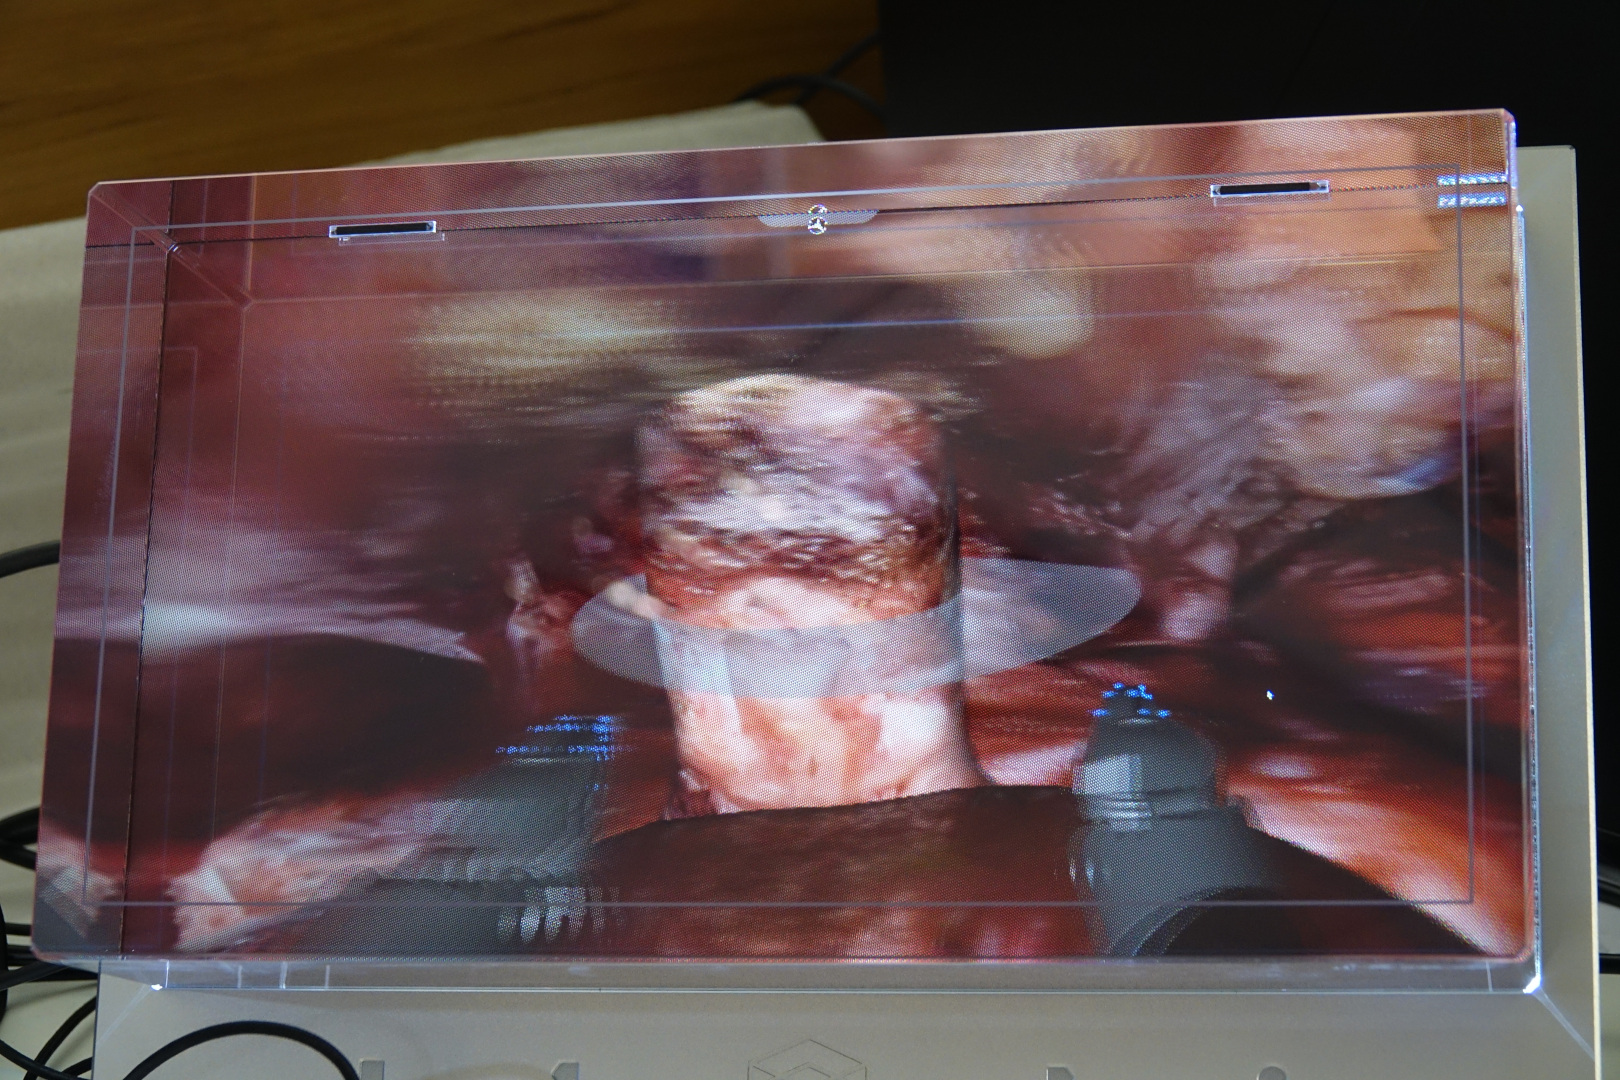
\includegraphics[width=0.75\textwidth,frame]{integration/looking_glass}
  \caption{The simulator scene being visualized in the large variant of the Looking Glass}
  \label{fig:looking_glass}
\end{figure}

\subsubsection{\acr{sofa} Integration}
\acr{sofa} is a widely used simulation framework, especially for medical simulations. We wanted to replicate the surgical scenario in \acr{sofa} to benchmark it against our implementation. We also wanted to investigate the added value of \acr{sofa} such as its fast prototyping capabilities by using \acr{xml}-based scene building and using Python scripting to customize behavior and apply modifications rapidly.

To recreate a similar environment in \acr{sofa}, we wanted to create or use existing \acr{sofa} capabilities to replicate the core functionalities of our simulator. \acr{sofa} comes bundled with plugins for tool simulation, mesh deformation, and cutting simulation. However, \acr{sofa} did not have an \acr{ovm} loader for loading volumetric tetrahedral meshes that we use in our simulator for deformable models. It also did not have support for UV-map-based texturing for volumetric meshes.

We were able to successfully develop plugins that enable us to load tagged \acr{ovm} meshes along with custom properties such as UV coordinates for the surface triangles and use it to apply UV-mapped textured to the volumetric meshes.

\begin{figure}
  \centering
  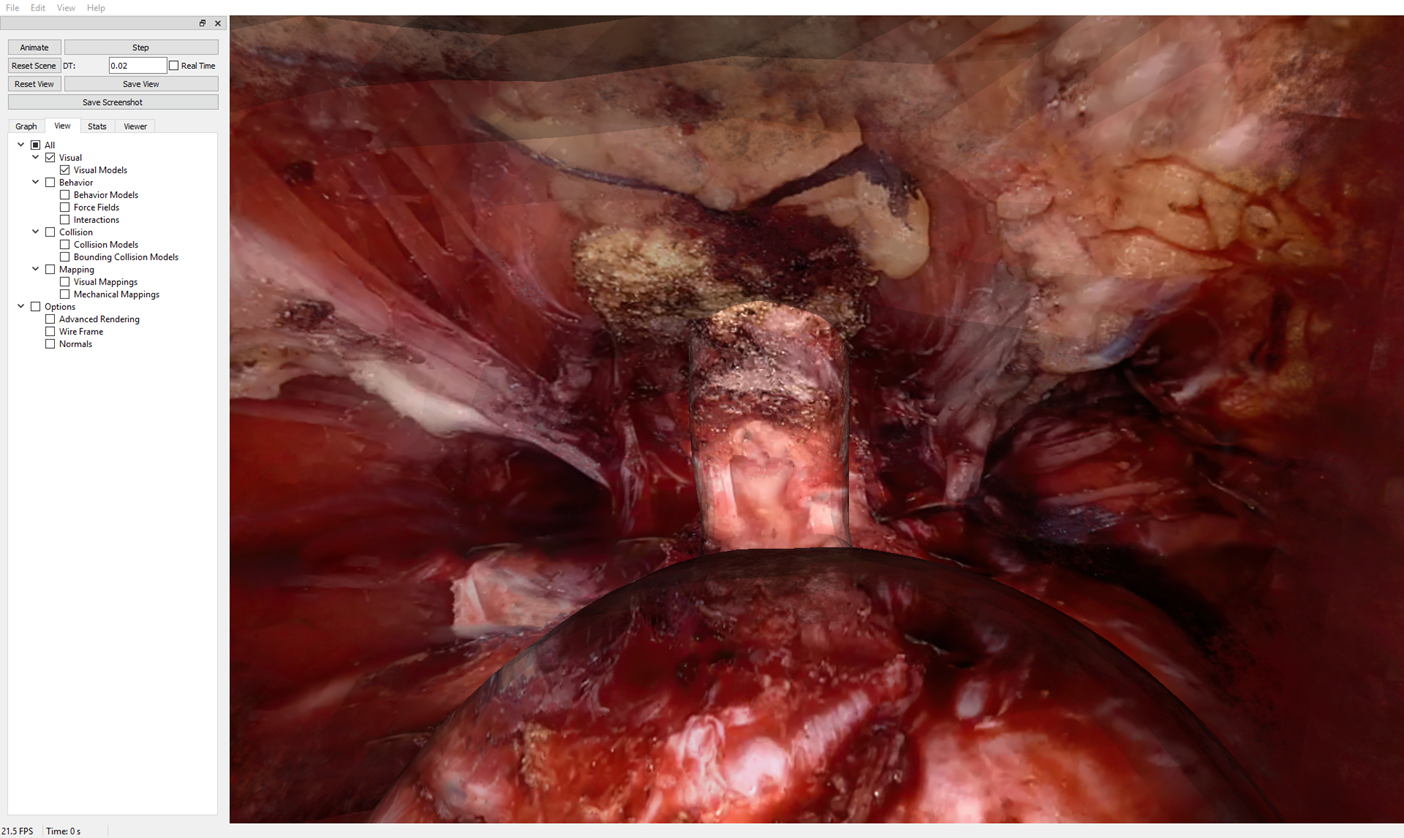
\includegraphics[width=1.0\textwidth,frame]{integration/sofa_preview}
  \caption{\acr{ovm} meshes loaded and textured in \acr{sofa}}
  \label{fig:sofa_preview}
\end{figure}

\subsubsection{Simulation Software Architecture}
\label{sec:software_architecture}
Our simulation software architecture is a modular and layered architecture. Each module of the software is responsible for one major task of the system.

Following are the major components of our simulator:
\begin{enumerate}
  \item Collision Detection and Physics Module: This module is responsible for detecting collisions between different simulation objects in the system. It also controls the  physics of the simulation.
  \item Cutting Module: Another important component of the system which is responsible for simulating the cutting of the mesh. Refer to \autoref{sec:cutting_system} for more details.
  \item Camera Module: Simulates stereoscopic cameras. This module is responsible for rendering, zooming, rotating, \etc.
  \item Rendering Module: Responsible for rendering the whole simulation to screen. (\acr{gui} + Simulation).
  \item Mesh Module: The 3D object to be simulated is represented via a mesh in the computer graphics world. This module is responsible for reading, manipulating, and writing the 3D mesh in the system.
  \item User Event Handler Module: This module is responsible for handling user events to control the system.
  \item Reporting Module: This module is responsible for collecting metrics while user is using the system and reporting it back when needed. This module also reports results of the simulations back to the user.
  \item Utilities Module: This module provides different utilities to the other modules to achieve their tasks. This is a helper module. It provides utilities like logging user events, logging flow of software, file reading, file writing, \etc.
  \item Replay Module: This module keep recording the current events and provide a way to replay the scenario executed by the user later on. This helps in debugging the software if any issues occur.
\end{enumerate}

\autoref{fig:software_architecture} shows a diagrammatic view of the software architecture of the simulation system.
\begin{sidewaysfigure}
  \centering
  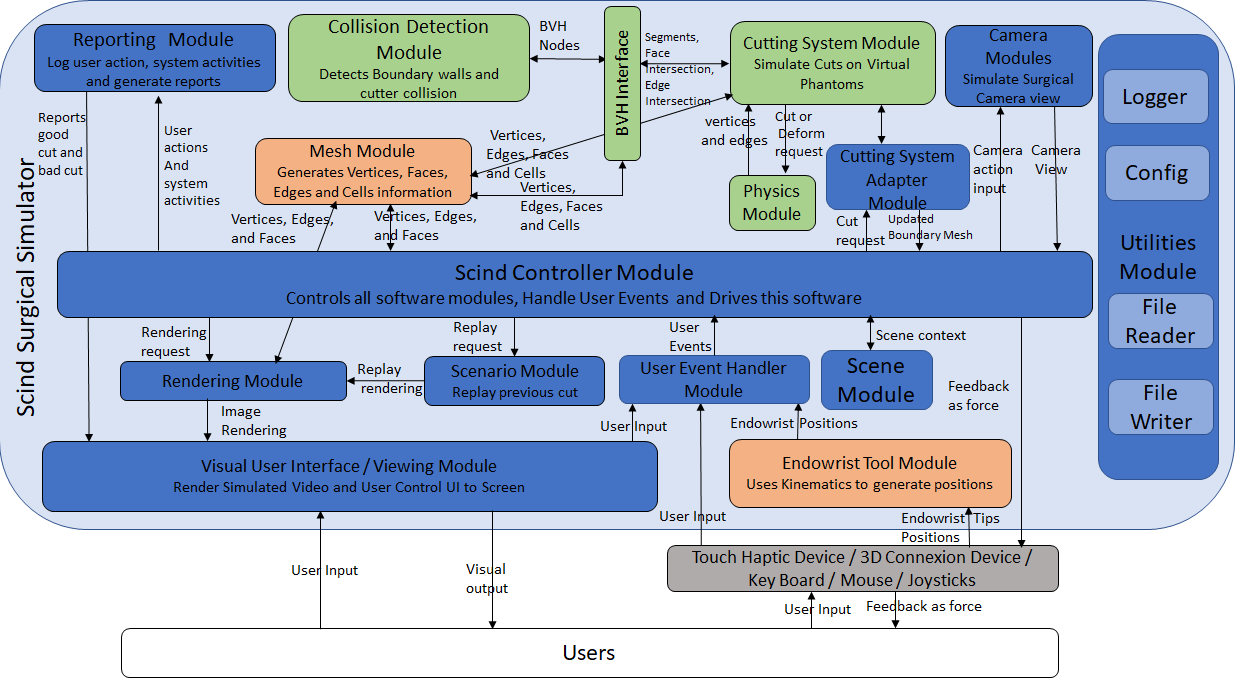
\includegraphics[width=1.0\textheight]{integration/swArchitectureScind}
  \caption{Surgical simulation software architecture}
  \label{fig:software_architecture}
\end{sidewaysfigure}

\subsubsection{Cutting System}
\label{sec:cutting_system}
The cutting system module is one of the important software module of the simulation software system whose main responsibility is to perform the cut in a volumetric mesh. It takes a volumetric mesh and cut geometry as input and processes the cut. Finally it update the volumetric mesh with updated information so that the physics  module as well as the rendering module can use it for the simulation. Cut geometry can be either cut surface triangles or traversal point paths. At a very high level, the cutting system performs the following tasks:
\begin{enumerate}
  \item Initialize the cut geometry
  \item Use a \acr{bvh} for edge intersection and face piercing and unpack the information
  \item Transfer the intersection information to the mesh
  \item Extract affected and active cells (for progressive cuts only) \item Process the cut (subdivisions)
  \item Do the mesh simplification
  \item Delete isolated cells, vertices, edges, and faces
  \item Collect deltas
  \item Update \acr{bvh} tree
  \item Update the mesh
\end{enumerate}

\autoref{fig:cutting_system} shows a flowchart of the cutting system algorithm.
\begin{figure}
  \centering
  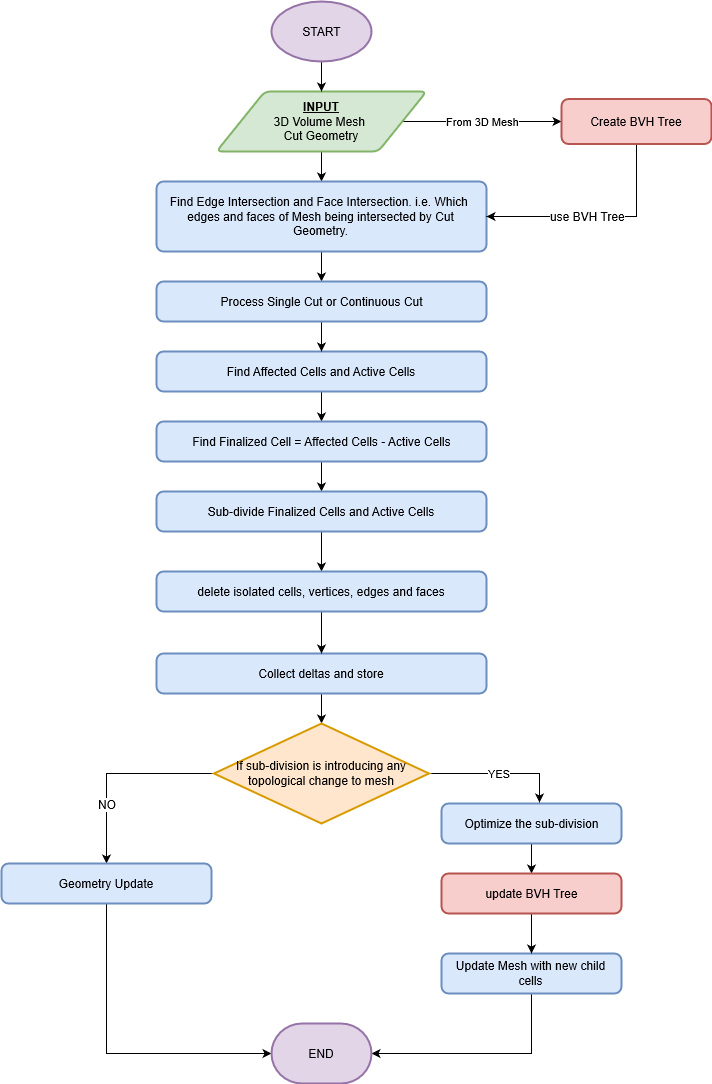
\includegraphics[width=0.9\textwidth]{integration/cutting_system}
  \caption{Cutting system overall flowchart}
  \label{fig:cutting_system}
\end{figure}

\subsubsection{Surgical Simulator Installer}
\label{sec:installer}
Easy deployment of the software saves both cost and time. Also with easy deployment mechanism like single click installer, it is easy to transfer the software across the globe and setup the system with compatible hardware. Our simulator software has external dependencies, drivers, and \acr{3d} mesh files. So, it is important to package them together so that it can be run and used on any laptop/workstation. For this reason, we developed a single click installer using Nullsoft scripting which packages all the needed components. To run Surgery Simulator we have to install Surgery Simulator Software using Surgical Simulator Installer, install 3D Touch drivers, and connect two 3D Touch Omni's. In conclusion, it is much easier to set up the Surgery Simulator System for demos using this installer. Note that this installer is only available for Windows. It also be used for uninstallation. \autoref{fig:installer} shows a picture of Surgical Simulator Installer while installing the software.

\begin{figure}
  \centering
  \thesubfigure{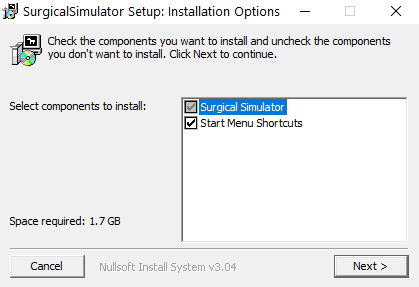
\includegraphics[width=0.45\textwidth]{integration/installer1}}\qquad
  \thesubfigure{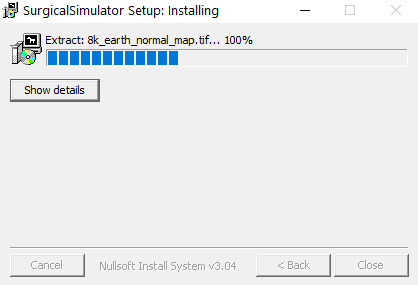
\includegraphics[width=0.45\textwidth]{integration/installer2}}
  \caption{Surgical simulator installer}
  \label{fig:installer}
\end{figure}

\clearpage%
